\documentclass[sigconf, anonymous,review]{acmart}
% \documentclass[manuscript, screen, review]{acmart}.
% \fancyhf{} % Remove fancy page headers 
% \fancyhead[C]{Anonymous submission \#9999 to ACM CCS 2019} % TODO: replace 9999 with your paper number
% \fancyfoot[C]{\thepage}
\AtBeginDocument{%
  \providecommand\BibTeX{{%
    Bib\TeX}}}
    
\setcopyright{none}
\copyrightyear{2023}
\acmYear{2023}
\acmDOI{XXXXXXX.XXXXXXX}
\acmPrice{15.00}
\acmISBN{978-1-4503-XXXX-X/23/11}
\acmSubmissionID{118}
% \setcopyright{none} % No copyright notice required for submissions
\acmConference[ACM CCS 2023]{ACM Conference on Computer and Communications Security}{November 26--30 2023}{Copenhagen, Denmark}
% \acmConference[ACM CCS 2023]{Make sure to enter the correct
%   conference title from your rights confirmation emai}{June 03--05,
%   2018}{Woodstock, NY}
\settopmatter{printacmref=false, printccs=true, printfolios=true} % We want page numbers on submissions

%%\ccsPaper{9999} % TODO: replace with your paper number once obtained
\usepackage{xspace}
\usepackage{xcolor}             % colors
\usepackage{booktabs}
\usepackage[ruled,linesnumbered,noend]{algorithm2e}               % Algorithm
\usepackage[capitalize,noabbrev]{cleveref}              %cross-reference
\usepackage{multirow}               %table
\usepackage[mathscr]{eucal}
\usepackage{bbding}             % signal
\usepackage{array}
\usepackage{listings}               %code
\usepackage{caption}
\usepackage{subcaption}
% \newtheorem{theorem}{Theorem}               %theorem
\lstset{
    language=SQL,
    basicstyle          =   \ttffamily,          
    keywordstyle        =   \color{blue},         
    commentstyle        =   \rmfamily\itshape,  
    stringstyle         =   \ttfamily,  
    flexiblecolumns,                
    % numbers             =   left,   
    showspaces          =   false,  
    numberstyle         =   \tiny,    
    showstringspaces    =   false,
    captionpos          =   t,      
    frame               =   lrtb,
}

\usepackage{amsmath,amssymb,booktabs}


% \newcommand{\NAME}{HE\mathop{$^{3}$}DB\xspace}
\newcommand{\NAME}{HE$^3$DB\xspace}
\newcommand{\tabincell}[2]{\begin{tabular}{@{}#1@{}}#2\end{tabular}}
\newcommand{\abs}[1]{\lvert {#1} \rvert}
\newcommand{\reg}[1]{{\rm {#1}}}
\newcommand{\step}[1]{$\bullet$ \textbf{#1}}
\newcommand{\yeah}{{\Checkmark}}
\newcommand{\nope}{{\textcolor{red}\XSolidBrush}}
\newcommand{\eyeah}{{\textcolor{blue}{\Checkmark}}}
\newcommand{\noyeah}{{\TriangleUp}}
\newcommand{\revise}[1]{\textcolor{blue}{{#1}}}
\newcommand{\etal}{{\it{et al.}}}
% SQL--------------------------------
\newcommand{\select}{\texttt{SELECT}}
\newcommand{\sort}{\texttt{Sort}}
\newcommand{\groupby}{\texttt{GROUP BY}}
\newcommand{\join}{\texttt{JOIN}}
\newcommand{\orderby}{\texttt{ORDER BY}}
\newcommand{\attribute}{\mathsf{Attr}}
\newcommand{\dbmin}{\texttt{MIN}}
\newcommand{\dbmax}{\texttt{MAX}}
\newcommand{\dband}{\texttt{AND}}
\newcommand{\dbnand}{\texttt{NAND}}
\newcommand{\dbnor}{\texttt{XOR}}
\newcommand{\dbnot}{\texttt{NOT}}
\newcommand{\dbtopk}{\texttt{Top-k}}
\newcommand{\dbsum}{\texttt{SUM}}
\newcommand{\dbavg}{\texttt{AVG}}
\newcommand{\dbcount}{\texttt{COUNT}}
\newcommand{\dbop}{\texttt{OP}}
\newcommand{\msb}{\texttt{MSB}}
\newcommand{\lsb}{\texttt{LSB}}
\newcommand{\calgo}{\texttt{Analysis}}
% \newcommand{\pdte}{\texttt{PDTE}}
\newcommand{\algoweight}{\mathsf{W}}

% HE---------------------------------
\newcommand{\homcomp}{\texttt{HomComp}}
\newcommand{\homgate}{\texttt{HomGate}}
\newcommand{\hmsb}{\texttt{HMSB}}
\newcommand{\cmux}{\texttt{CMUX}}
\newcommand{\br}{\texttt{BlindRotate}}
\newcommand{\pbs}{\texttt{PBS}}
\newcommand{\pbshmsb}{\texttt{PBS-HMSB}}
\newcommand{\sei}{\texttt{RLWEtoLWEs}}
\newcommand{\repack}{\texttt{LWEstoRLWE}}
\newcommand{\cb}{\texttt{LWEtoRGSW}}
% \newcommand{\homgate}{\texttt{HomGate}}
\newcommand{\lwe}{{\mathsf{LWE}}}
\newcommand{\lwenan}{{\mathsf{LWE_{\rm NaN}}}}
\newcommand{\rlwe}{{\mathsf{RLWE}}}
\newcommand{\rlweslot}{{\mathsf{RLWE\text{-}Slot}}}
\newcommand{\rlwecoeff}{{\mathsf{RLWE\text{-}Coeff}}}
\newcommand{\rrlwe}{{\mathsf{R}/\mathsf{LWE}}}
\newcommand{\rgsw}{{\mathsf{RGSW}}}
\newcommand{\gsw}{{\mathsf{GSW}}}
\newcommand{\rrgsw}{{\mathsf{R}/\mathsf{GSW}}}
\newcommand{\ttr}{{\Tilde{r}}}
\newcommand{\ttp}{{\Tilde{p}}}
\newcommand{\ttm}{{\Tilde{m}}}
\newcommand{\tts}{{\Tilde{s}}}
\newcommand{\ttv}{{\Tilde{v}}}
\newcommand{\frakt}{{\mathfrak{t}}}
\newcommand{\ba}{{\mathbf{a}}}
\newcommand{\bs}{{\mathbf{s}}}
\newcommand{\bm}{{\mathbf{m}}}
\newcommand{\bb}{{\mathbf{b}}}
\newcommand{\bBK}{{\mathbf{BK}}}
\newcommand{\kcmux}{{\texttt{1-out-of-k-CMUX}}}
\newcommand{\cmp}{{\texttt{cmp}}}
\newcommand{\hommin}{{\texttt{HomMIN}}}
\newcommand{\hommax}{{\texttt{HomMAX}}}
\newcommand{\homminagg}{{\texttt{HomMINAgg}}}
\newcommand{\hommaxagg}{{\texttt{HomMAXAgg}}}
\newcommand{\encode}{\mathcal{E}}
\newcommand{\prnd}{p_{\rm Round}}
\newcommand{\homlt}{{\texttt{HomLT}}}

% Notation---------------------------

\newcommand{\db}{\mathcal{D}}
\newcommand{\dbabs}{\abs{\mathcal{D}}}
\newcommand{\dbtab}{\mathcal{T}}
\newcommand{\dbabstab}{\abs{\mathcal{T}}}
\newcommand{\dbtabrow}{|\mathcal{T}|_{\rm row}}
\newcommand{\dbtabcolumn}{|\mathcal{T}|_{\rm row}}
\newcommand{\dbquery}{\mathcal{Q}}
\newcommand{\dbabsquery}{\abs{\mathcal{Q}}}

\newcommand{\dbtabrowsize}{|\mathcal{T}|_{\rm row}}
\newcommand{\dbtabcolsize}{|\mathcal{T}|_{\rm col}}
\newcommand{\upint}[1]{\left \lceil {#1} \right \rceil}
\newcommand{\round}[1]{\left \lceil {#1}  \right \rfloor}
\newcommand{\Round}{\texttt{Round}}

\newcommand{\pdte}{\texttt{PDTEval}\xspace}

\begin{document}
%\title{HDB: Homomorphic Encrypted Database via Arithmetic-and-Logic Circuit} % TODO: replace with your title
\title[\NAME: An Efficient Encrypted Database via Fully Homomorphic Encryption]{\NAME: An Efficient and Elastic Encrypted Database Via
Arithmetic-And-Logic Fully Homomorphic Encryption}
%\\ Secure and Efficient Analytical Data Processing} % TODO: replace with your title
\begin{abstract}
% Cloud-based database management systems (DBMS) allow users to manage and
% analyze data in a convenient way while leaking their sensitive information.
% Modern cloud-based database management systems (DBMS) generally store 
% data from the clients in a decipherable manner, where the data
% are either kept completely in plaintext or in ciphertext but with a secret key 
% that is known to the cloud vendor.
% Meanwhile, 
% Along with the strengthened regulations over on data privacy protection, 
As concerns are increasingly raised about data privacy,
encrypted database management system (DBMS) based on fully homomorphic 
encryption (FHE) attracts increasing research attention, as FHE permits DBMS 
to be directly outsourced to cloud servers without revealing any plaintext data. 
However, the real-world deployment of FHE-based DBMS faces two main challenges: 
i) high computational latency, and ii) lack of elastic query processing capability, 
both of which stem from the inherent limitations of the underlying FHE operators.
Here, we introduce \NAME, a fully homomorphically encrypted, 
efficient and elastic DBMS framework based on a new FHE infrastructure.
By proposing and integrating new arithmetic and logic homomorphic operators,
we devise fast and high-precision homomorphic comparison and aggregation algorithms
that enable a variety of SQL queries to be applied over FHE ciphertexts, 
e.g., compound filter-aggregation, sorting, grouping, and
joining. In addition, in contrast to existing encrypted DBMS that only support
aggregated information retrieval, our framework permits further server-side 
analytical processing over the queried FHE ciphertexts, such as private
decision tree evaluation.
In the experiment, we rigorously study the efficiency and flexibility of 
\NAME. We show that, compared to the state-of-the-art techniques,
\NAME can homomorphically evaluate end-to-end SQL queries 
as much as $41\times$--$299\times$ faster than the state-of-the-art solution,
completing a TPC-H query over a 16-bit 10K-row database within 241 seconds.
%$34\times$ faster sorting, and zz$\times$--rr$\times$ faster decision tree evaluation,

\end{abstract}

% In this work, we delve into such a problem, encrypted database management system (EDBMS) -
% where a client wants to manage and analyze her data without revealing the data 
% to the cloud service provider. 
% , significantly improving the practical applicability 
% of FHE-based DBMS.
% to evaluate aggregation queries containing 
% unbounded filter predicates without decryption. 
% Furthermore, we design a mechanism for querying and analyzing data in encrypted 
% To add: 
% To the best of our knowledge, this is the first work that supports homomorphic decision trees in encrypted databases where both the data and the model are in encrypted form.
% As part of our design, we solve multiple cryptographic problems related to FHE
% DBMS bridge the gap between data queries and data analysis by supporting both data management and application constructions.

\sloppy
% \begin{CCSXML}
% <ccs2012>
%    <concept>
%        <concept_id>10002978.10003018.10003020</concept_id>
%        <concept_desc>Security and privacy~Management and querying of encrypted data</concept_desc>
%        <concept_significance>500</concept_significance>
%        </concept>
%  </ccs2012>
% \end{CCSXML}

% \ccsdesc[500]{Security and privacy~Management and querying of encrypted data}
% \begin{CCSXML}
% <ccs2012>
%    <concept>
%        <concept_id>10002978.10002979</concept_id>
%        <concept_desc>Security and privacy~Cryptography</concept_desc>
%        <concept_significance>500</concept_significance>
%        </concept>
%    <concept>
%        <concept_id>10002978.10003018.10003020</concept_id>
%        <concept_desc>Security and privacy~Management and querying of encrypted data</concept_desc>
%        <concept_significance>300</concept_significance>
%        </concept>
%  </ccs2012>
% \end{CCSXML}


% \ccsdesc[500]{Security and privacy~Cryptography}
% \ccsdesc[300]{Security and privacy~Management and querying of encrypted data}


\begin{CCSXML}
<ccs2012>
   <concept>
       <concept_id>10002978.10002979</concept_id>
       <concept_desc>Security and privacy~Cryptography</concept_desc>
       <concept_significance>500</concept_significance>
       </concept>
   <concept>
       <concept_id>10002978.10003018.10003020</concept_id>
       <concept_desc>Security and privacy~Management and querying of encrypted data</concept_desc>
       <concept_significance>500</concept_significance>
       </concept>
 </ccs2012>
\end{CCSXML}

\ccsdesc[500]{Security and privacy~Cryptography}
\ccsdesc[500]{Security and privacy~Management and querying of encrypted data}
\keywords{Encrypted Database, Homomorphic Encryption, Privacy} % TODO: replace with your keywords
\keywords{Fully Homomorphic Encryption, Secure Database Outsourcing}
\maketitle

\section{Introduction}
Outsourcing the storage of and computation over private data to cloud service
providers~\cite{amazon_aws,microsoft_sql,monogb_sql,google_sql} 
is a common practice for personal users, enterprises, and even government
institutions to lift the burden of large-scale data management.
However, in many cases, the outsourced data contain sensitive information, and
data owners are concerned with their private data either
directly stolen by the curious cloud service providers~\cite{lu2019assessing} or 
leaked through the endless data breaches~\cite{trautman2017corporate,
cadwalladr2018revealed}.  As a result, data owners
and cloud service providers are interested in building encrypted 
database infrastructures~\cite{poddar12arx}, where the entire database is stored 
in ciphertext on the cloud. 
However, due to the inherent complexity in the design
of multi-party secure protocols, 
the fundamental challenge confronting encrypted databases is on how to efficiently 
and elastically process queries on the encrypted data outsourced to the cloud while preventing 
various side channel leakages~\cite{cash2015leakage,grubbs2018pump, attackSOD}.
% What the past decade witnessed is a period of fast development in database
% management systems (DBMS) as a cloud-based service, which provides not only
% data storage and queries, but also business operational analytics and machine
%learning (ML) predictions to get a deeper insight into data
% However, such cloud-based DBMS requires users to provide their sensitive data, 
% like financial transactions and medical records, and may lead to data breaches due
% to the cyber-attacks or the illegal use of data by database administrators (DBA).
% Give rise to encrypted database


% Unfortunately, many of the above protocols are designed to be {\it{application-specific}}.
% In other words, due to security, data compatibility, and efficiency reasons, 
% it can be challenging to combine different database functionalities
% into a unified framework.

\begin{figure}[t!]
   \begin{center}
   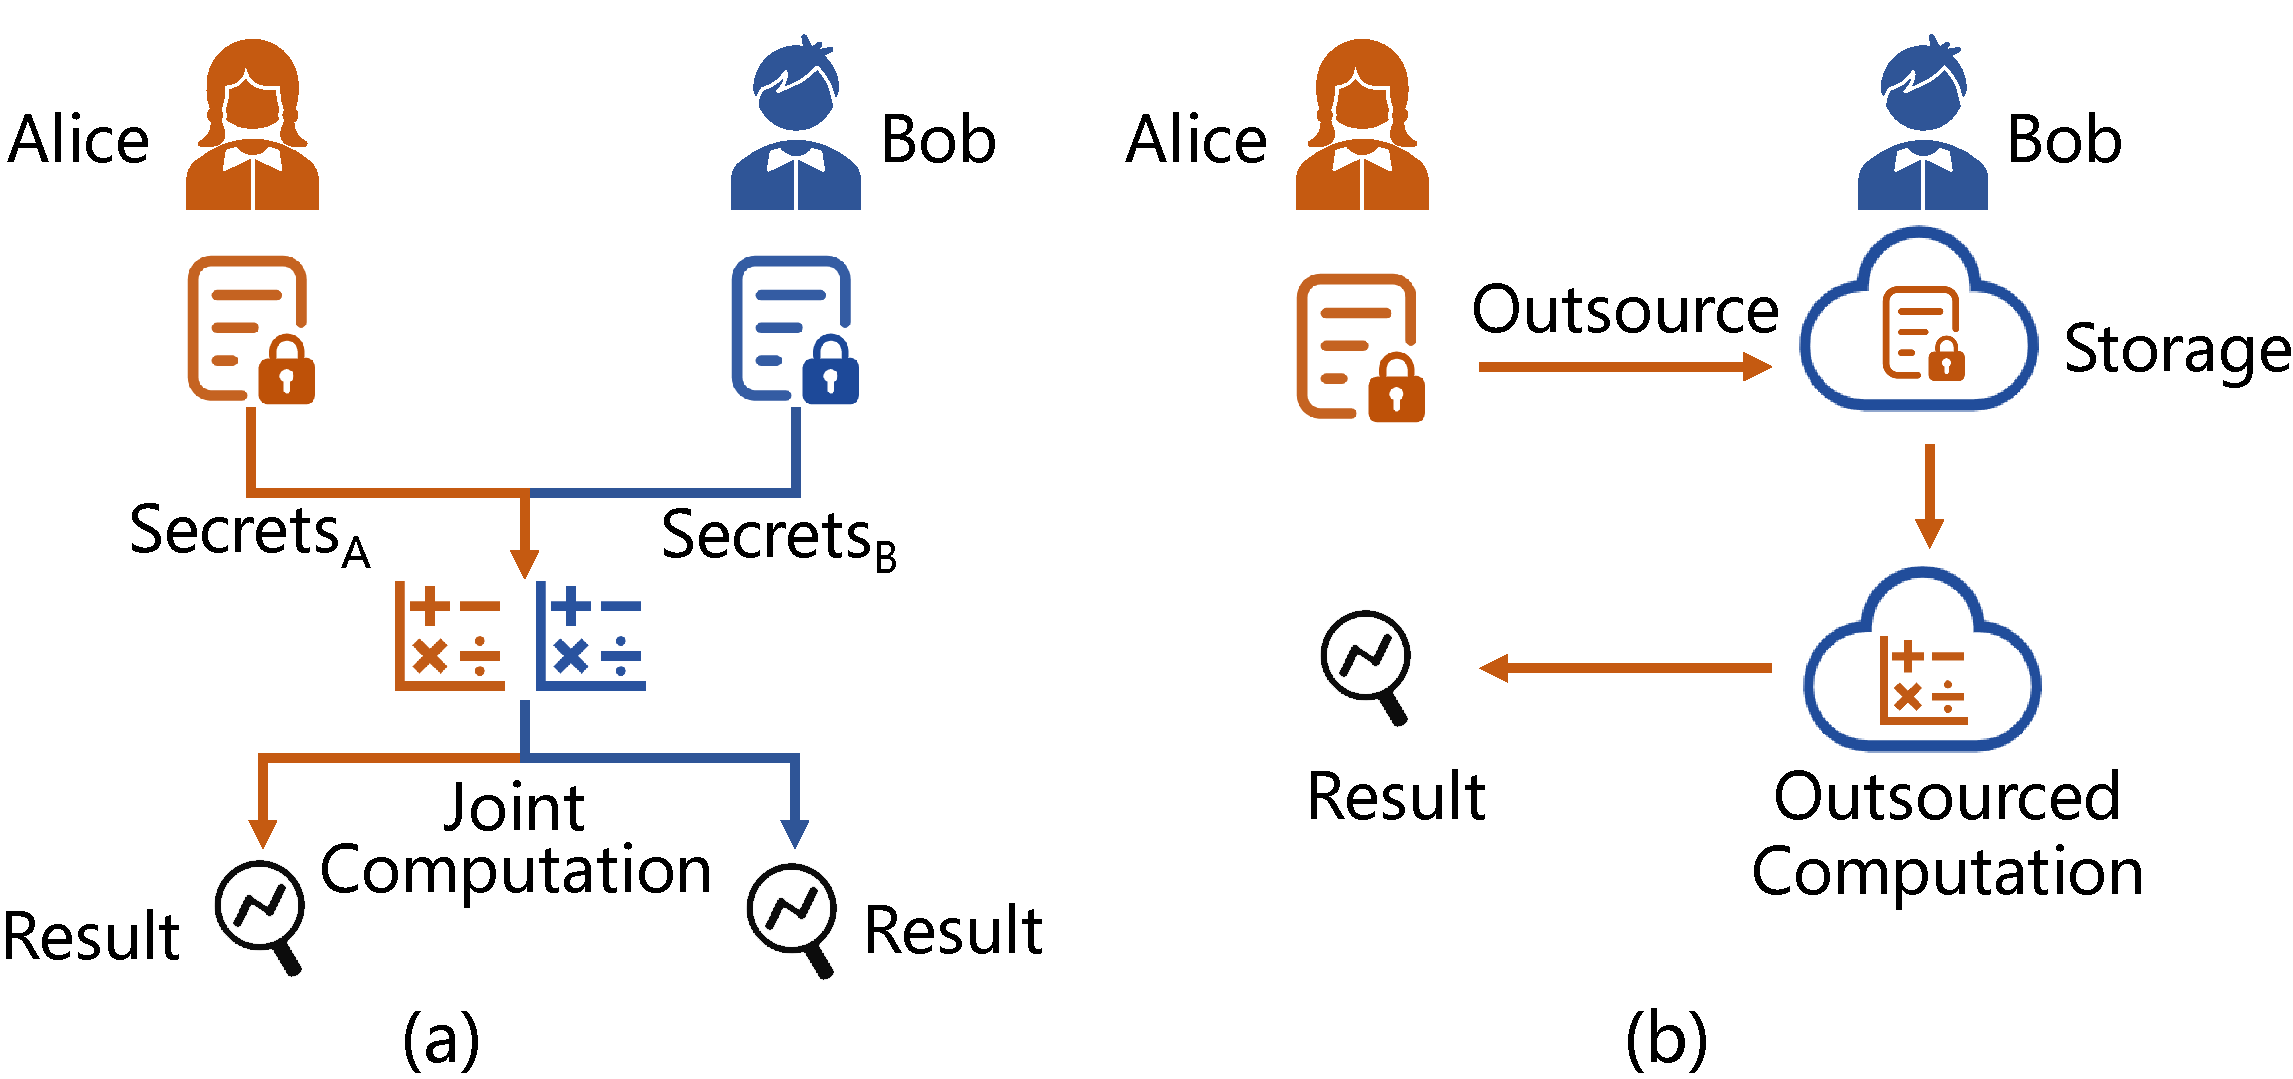
\includegraphics[width=1\linewidth]{figure/sdonsqe.pdf}
   \end{center}
      \caption{The conceptual illustrations of (a) a secure
      multi-party query evaluation (SQE) scheme and (b) a
      secure database outsourcing (SDO) scheme.} 
   \label{fig:threat}
   % \vspace{-0.5em}
\end{figure}

To tackle the above challenges, existing works propose different designs of encrypted
databases that utilize tools across multiple fields of 
research~\cite{sagma,eskandarian2017oblidb,priebe2018enclavedb,esolute,yi2012single,wang2021secure,liagouris2021secrecy,poddar2021senate,waldo,heda}.
% Depending on the targeting threat model, encrypted databases
% are constructed over a plethora of cryptographic or secure computing methods, 
% including those based on
% oblivious random access machine (ORAM)~\cite{oblidb}, searchable encryption 
% (SE)~\cite{sagma}, trusted execution environment 
% (TEE)~\cite{eskandarian2017oblidb,priebe2018enclavedb}, differential privacy~\cite{esolute}, 
% private information retrieval~\cite{yi2012single}, private set intersection~\cite{wang2021secure}, 
% and secure multi-party computing  (MPC)~\cite{liagouris2021secrecy, poddar2021senate, waldo, heda}.
We categorize existing designs of encrypted databases
into two types of protocol models: secure multi-party query evaluation (SQE) and 
secure database outsourcing (SDO).
% encrypted databases 
% by whether hardware trusted execution environment (TEE) is adopted and 
% whether the presumed threat model is .  
As illustrated in \cref{fig:threat}, we assume that no party 
in an SQE protocol can recover all of the secrets only by its own.
In contrast, SDO refers to the case where one of the participating parties 
(e.g., the one who outsources the data) owns all of the private data. 
Thus, even though both SQE and SDO prefer lower
protocol overheads, parties involved in SQE are willing to pay more
computation and communication costs in the exchange of being
able to compute over unknown secrets. Meanwhile, for SDO, client-side workloads need
to be strictly smaller than that without the protocol, otherwise the client
can simply perform the computations locally on its own.
% SDO is defeated.

With the optimal round complexity~\cite{mukherjee2016two} and
low online communication, fully homomorphic encryption (FHE) 
emerges as a powerful cryptographic primitive for SDO.
% Since arbitrary computations can be executed on the homomorphically encrypted 
While FHE was deemed too slow to DB applications~\cite{shan2018practical}, 
recent advances in FHE 
cryptography~\cite{conversionhaochen, revisiting, pegasus, meta-bts}
have significantly improved the efficiency and operator usability of FHE,
leading to a series of recent works exploring the practical feasibility
of FHE in DB-related tasks~\cite{pegasus,cong2021labeled,heda}.
For instance, the very recent work HEDA~\cite{heda} employs FHE schemes including the 
BFV~\cite{DBLP:conf/crypto/brakerski12,DBLP:journals/iacr/FanV12} and 
TFHE~\cite{DBLP:journals/joc/ChillottiGGI20}  
to accelerate filter-aggregation queries over fully homomorphically 
encrypted database. Unfortunately, in addition to the relatively
slow evaluation speed, HEDA suffers from limited query expressiveness
% the computational costs of HEDA remain relatively high as a single ciphertext 
% format conversion 
% from the filtering mode to the aggregation mode requires 9 seconds~\cite{heda},
% which translates to a query latency of more than 100 days over a DB with one 
% million rows. In addition, as mentioned in~\cite{heda},
as the exact algorithmic constructions for the evaluations of many 
common SQL statements, such as $\dbmin$, $\dbmax$, $\join$ and $\orderby$,
are left as open questions~\cite{heda}. %, limiting the query expressiveness of HEDA.
% Data analysis capabilities 
% to be performed on the aggregated results, due to the lack of efficient homomorphic
% conversion algorithms. 
Therefore, the main challenge faced by FHE-based SDO becomes the following question:
can we design an encrypted database scheme over FHE that achieves both fast query 
evaluation and elastic data processing at the same time?
% Therefore,
% despite that homomorphic encryption (HE) has been traditionally employed in building
% both SQE~\cite{chen2017fast,poddar2021senate} and 
% SDO~\cite{cryptdb, poddar12arx,sagma,aphadb},
% most designs only adopts partially or leveled homomorphic encryption schemes instead
% of adopting an FHE setup. However, along with the 
% FHE-based encrypted database 
\subsection{Our Contribution}
In this work, we propose \NAME, 
an FHE-based encrypted DBMS for fast and elastic SDO. 
We observe that most existing FHE algorithms, 
whether specifically designed for SDO~\cite{heda} or not~\cite{pegasus,ckkscomparison}, 
do not fully capture the important properties of encrypted databases,
and often fail to meet the key requirements of SDO.
%Different from the general FHE algorithms suggested by existing work,
Contrarily, based on the idea of application-framework co-design, 
we propose a tailored FHE infrastructure consisting of DB-specific
FHE operators that leverage the numerical and operational characteristics
specific to encrypted databases. As it turns out, we are able to
achieve higher accuracy, faster evaluation speed, richer query expressiveness
and better security all at once.
% By devising a set of new cryptographic 
% tools, \NAME is able to evaluate one of the most complete sets
% of SQL statements under an SDO setting, at speeds that are $10$--$100\times$ faster
% than the respective existing solutions. 
In addition, to the best of our knowledge,
\NAME is the first FHE-based DB framework that enables a client to
execute outsourced data analysis algorithms on the queried ciphertext results 
without additional rounds of client-server 
interactions.
% , which is a key feature for many outsourced DBMS that is
% missing in existing solutions~\cite{heda}.
%, using complex learning algorithms such as private decision tree. 

% The main contributions of this work are summarized as follows.
% that achieves low computation cost and storage in the DBMS 
% provider and unbound number of filtering predicates and aggregations analysis. 
% outsourced, complete, 

% \vspace{0.03in}
\noindent
\begin{itemize}
    \item {\bf{An FHE Infrastructure for Encrypted DBMS}}:
    % We decompose the SQL queries into a set of fundamental arithmetic and 
    % logic functions, and design DB-specific FHE operators to efficiently 
    % realize such functions.
    We develop novel homomorphic filtering, aggregation and
    conversion algorithms that are highly composable and specifically designed
    for various types of DB operands and complex SQL operations.
    As a result, \NAME supports one of the most complete sets 
    of SQL statements 
    for encrypted databases, along with online data analysis capability.
    % , including unbounded-depth filter-aggregation, grouping, sorting,
    % and joining of encrypted DB items. 
    % a new FHE infrastructure needs to be constructed to handle the complex 
    % queries over databases. 
    % In particular, multiple FHE ciphertext formats need to 
    % co-exist,  and efficient conversion algorithms need to be installed .
    %FHE -> algorithm -> framework
    \item {\bf{High-Precision Homomorphic Comparison}}: 
    We observe that, the key FHE operator for encrypted database is
    the high-precision homomorphic comparison operator. 
    However, the result of a homomorphic comparison is always binary.
    Based on the above insight, we devise a new shift-and-subtract strategy
    to homomorphically remove the lower-bit noises from the comparison results,
    and develop a high-precision homomorphic comparison operator $\homcomp$.
    %by subsequent DB aggregations. 
    %Our $\homcomp$ operator can
    We can evaluate homomorphic comparison with up to 32-bit precision without using
    bit-by-bit encryption.
    % and are able to carry out
    % fast homomorphic comparisons between inputs that are both ciphertexts encrypting
    % up to 32-bit precision plaintext messages, without relying on bit-by-bit encryption.
    %achieving the highest level of accuracy to the best of our knowledge.
    % We obtain high precision comparison by iterating lower precision comparison.
    \item {\bf{Homomorphic Aggregations over Filtered Results}}:
    Based on the $\homcomp$ operator, we are able to propose fast algorithms to perform both 
    arithmetic (e.g., $\dbsum$, $\dbavg$)  and logic (e.g., $\dbmin$, $\dbmax$)
    aggregations on the filtered results. Our arithmetic and logic aggregation
    can be as much as $58\times$ and $34\times$ faster than existing works, respectively.
    % We note that most existing FHE-based DB designs~\cite{yi2012single,aphadb,heda}
    % do not simultaneously support arithmetic and logic aggregations
    
    %arithmetic and logic aggregation, efficient
    
    \item {\bf{Thorough Experiments}}: 
    We show that \NAME achieves $7\times$--$113\times$ faster homomorphic
    filtering, $23\times$--$58\times$ faster homomorphic aggregation,
    $34\times$ faster $\orderby$, and $12\times$--$326\times$ 
    faster private decision tree evaluation, 
    all against the best-performing implementations. In addition,
    we show that \NAME is on average $41\times$--$299\times$
    faster than the state-of-the-art FHE-based DBMS over end-to-end SQL benchmarks. 
    A demo for the 
    end-to-end TPC-H~\cite{tpc_h} query evaluation process is submitted as a 
    proof-of-concept artifact for the proposed algorithms.
    % We plan to provide
    
    % a fully open source implementation \NAME\footnote{A demo of the 
    % end-to-end TPC-H~\cite{tpc_h} query evaluation process is submitted as a proof-of-concept artifact 
    % for the proposed algorithms.}.
\end{itemize}

\subsection{Related Works}\label{sec:relatedworks}
Here, we introduce existing works based on three main groups: 
trust-execution-environment-(TEE)-based SQE and SDO, 
MPC-based SQE, and MPC-based SDO. Note that, here, we consider FHE
to be one particular type of general MPC technique.

% {\bf{TEE-based SDO and SQE}}: 
\subsubsection{TEE-based SDO and SQE}
%It is obvious that there are many advantages of adopting
%hardware enclaves in instantiating encrypted databases: high processing speed,
%low communication overheads, high usability and rich query expressiveness. 
%In particular, 
TEE-based solutions can easily realize both
SDO and SQE simultaneously~\cite{bajaj2011trusteddb, arasu2015transaction, zheng2017opaque, 
eskandarian2017oblidb, priebe2018enclavedb, mishra2018oblix, bailleu2019speicher, 
kim2019shieldstore, vinayagamurthy2019stealthdb, antonopoulos2020azure, wang2022operon}. 
For example, although earlier techniques are constrained by the memory hierarchy of 
TEE~\cite{bajaj2011trusteddb,arasu2015transaction, priebe2018enclavedb}, newer 
TEE architectures have largely abandoned memory integrity verification, thereby 
removing the limit on memory size~\cite{johnson2021supporting, feng2021scalable}. 
Subsequently, recent TEE-based techniques~\cite{antonopoulos2020azure, wang2022operon} 
have demonstrated that advanced DBMS can be built over TEE with advanced access control mechanisms.
Unfortunately, TEE-based encrypted databases face two fundamental challenges.
First, the hardware architectural design of TEE can change significantly from one to 
the other, causing security vulnerabilities to be introduced. 
For example, as mentioned in~\cite{wang2022operon}, encrypted database based on Intel 
SGX~\cite{costan2016intel} 
can leak access pattern~\cite{eskandarian2017oblidb}, while that based on application-specific
TEE enclaves~\cite{suh2007aegis} do not.
% Meanwhile, even if the users are aware of the fact that
% the underlying hardware is insecure for their purpose, switching to a different hardware
% architecture can be too costly or even impossible in some highly customized applications.
Second, as a common critique for most privacy-preserving computing tasks 
based on TEE, it can be discouraging for applications that require
a high level of data confidentiality to adopt a hardware root of trust.
% Hence, while countermeasures such as~\cite{eskandarian2017oblidb} exist to reinforce 
% certain security properties of TEE-based solutions, encrypted databases based on
% TEEs can be insufficient to meet real-world data protection needs.
% {\bf{MPC-based SQE}}: 
\subsubsection{MPC-based SQE}
Most MPC-based encrypted databases focus on developing
methods to evaluate queries over contents that are owned by different participating
parties, e.g., ~\cite{bater2016smcql, ishai2016private, 
fuller2017sok, corrigan2017prio, volgushev2019conclave, 
demertzis2020seal, incshrink, liagouris2021secrecy, poddar2021senate, wang2021secure, waldo}. 
Due to the inherent complexity of SQE,  MPC protocols vary significantly in terms of 
their  security assumptions, 
security properties, efficiency, and usability. The main consequence of such a design 
complexity is that protocols tend to be incompatible with each other, and it can be 
very hard to integrate such protocols into a single database framework. 
For instance, the recent encrypted DB protocol Waldo~\cite{waldo} does
not support certain SQL 
operators such as $\groupby$ and $\join$~\cite{waldo}. 
Although many MPC-based protocols, such as Secure 
Yannakakis~\cite{wang2021secure}, Secrecy~\cite{liagouris2021secrecy} and 
Senate~\cite{poddar2021senate}, do support secure $\groupby$ and $\join$ operations, 
these protocols cannot be easily combined together because 
% of the distinct threat models and
% secure computing primitives. Concretely,
Secure Yannakakis~\cite{wang2021secure} is a two-party protocol that utilizes standard
secret sharing, while Waldo and Secrecy assume an honest-majority three-party setting built over
functional secret sharing~\cite{boyle2021function} and replicated secret 
sharing~\cite{araki2017optimized}.
% , while Senate guarantees full malicious security 
% under a many-party (i.e., more than three-party) setting that primarily relies on 
% garbled circuits. 
% Therefore, while MPC-based SQE techniques and frameworks 
% are under active research, the primary research focuses can 
% Therefore, the primary research focuses of MPC-based SQC can
% differ significantly, and it can be highly non-trivial to quantitatively
% compare \NAME to these works. 
In addition, since secrets are defined to be
distributed over the participating parties, MPC-based techniques generally
require a relatively large amount of communication bandwidth and interaction 
rounds~\cite{waldo}. For example, with proper GPU acceleration~\cite{watson2022piranha}, 
communication can be $6\times$--$1000\times$ slower than the computation in 
the state-of-the-art MPC protocols,
becoming the main latency bottleneck.

% {\bf{MPC-based SDO}}: 
\subsubsection{{MPC-based SDO}}
Different from SQE, methods for SDO explore
how to securely and efficiently {\it{outsource}} a database to an untrusted 
server~\cite{cryptdb,seabed,poddar12arx,sagma,aphadb,heda}. 
Existing MPC-based 
SDO schemes generally adopt more than one type of MPC primitives, including
ORAM~\cite{eskandarian2017oblidb}, SE~\cite{poddar12arx, seabed, sagma}, and 
homomorphic encryption~\cite{cryptdb, eskandarian2017oblidb, sagma}.
However, as mentioned earlier, protocols based on SE~\cite{curtmola2006searchable,cash2013highly} 
introduces side-channel
leakages~\cite{islam2012access,cash2015leakage,grubbs2018pump,grubbs2019learning,
gui2019encrypted}.
% which are crucial security vulnerabilities in realizing encrypted databases. 
Meanwhile, albeit ORAM~\cite{stefanov2018path} achieves poly-logarithmic complexity
in oblivious storing and retrieving data items, executing multi-dimensional 
operations over ORAM, such as sorting, incurs extensive communications
and interactions between the data owner and the cloud server that can be prohibitive
in data outsourcing applications. Finally, most MPC-based SDO adopts some sort of
homomorphic encryption, e.g., based on partially homomorphic
encryption~\cite{cryptdb,poddar12arx, seabed, sagma} or 
leveled homomorphic encryption~\cite{aphadb}. Unfortunately, 
without additional MPC primitives, both partially and leveled homomorphic
encryption result in limited query expressiveness 
and data analysis capability,
either due to complex query encoding schemes or {\it{a-priori}} bounds over
the encryption parameters.
% As also pointed out in related literature~\cite{shan2018practical}, 
% while SDO can be considered as a type of multi-party secure protocol, computation 
% outsourcing is fundamentally different from multi-party secure computing in terms of
% its threat model and protocol goal. 

% As a result, except for TEE-based solutions, 
% only a handful of works scrutinized methods to evaluate information-rich SQL 
% queries over outsourced database.  
% Finally, we point out that most SDO protocols are constructed over some sort 
% of homomorphic encryption schemes~\cite{cryptdb,seabed,sagma}. 

% {\bf{FHE-based SQE and SDO}}: 
\subsubsection{FHE-based SQE and SDO}
Different from partially and leveled homomorphic
encryption, FHE~\cite{DBLP:conf/crypto/brakerski12, DBLP:conf/innovations/bgv12, 
DBLP:journals/dcc/SmartV14, DBLP:conf/crypto/GentrySW13, DBLP:conf/eurocrypt/DucasM15,  
DBLP:journals/joc/ChillottiGGI20,  DBLP:conf/asiacrypt/CheonKKS17} 
is capable of evaluating complex queries over both outsourced and 
two-party secure databases\footnote{We note 
that SQE over single-key FHE is limited to a two-party setting, while more
complicated multi-party protocols require further advance in the
development of multi-key FHE schemes~\cite{peikert2016multi,mukherjee2016two,aloufi2021computing}.}.
Since FHE was extremely computationally expensive in the earlier 
days~\cite{cryptdb,shan2018practical},  protocols over FHE often only implement a
small subset of database-related operations, e.g., 
supporting PIR~\cite{yi2012single} or keyword search~\cite{khedr2015shield,oscc} only.
Recently, motivated by the notable progresses made in the development of
fast and flexible FHE primitives~\cite{pegasus, ckksbootvariance}, new FHE-based
SDO schemes are proposed, e.g.,~\cite{heda}. Nonetheless, in addition to the slower 
performance, 
the query expressiveness of \cite{heda} can be rather restricted,
as the scheme does not have support for common SQL statements such as
$\groupby$ and $\orderby$.
%and data analysis capability, diminishing the benefit of adopting FHE.
Hence, the key objective of this work is to significantly boost the 
computational performance of FHE-based encrypted database while retaining the
rich query expressiveness and unbounded data analysis capability of modern DBMS.

% for the computational overheads of FHE were extremely high.
% While recent works hints that improvements in FHE can potentially be 

% As a result,
% relatively heavy interactions and communications between participating parties for
% the exchange of secrets can be inevitable in MPC-based SQE protocols.

% The goal of SDO is solely to outsource the storage of and related processing over 
% private data.  



% As further discussed in \cref{sec:relatedworks}, while TEE-based solutions generally achieve
% superior computation and communication performance, hardware trust roots can be 
% , i.e., 
% the exchange of secrets {\it{must}} happen between parties for the completion of 
% the protocol. 

% That is the server executes queries on encrypted data and provides a 
% cloud-based encrypted database management system (EDBMS).
% The EDBMS can be thought of as a secure two-party computation (TPC) problem
% and a lot of exciting schemes, such as CryptDB~\cite{cryptdb}, 
% Seabed~\cite{seabed}, SAGMA~\cite{sagma}, IncShrink~\cite{incshrink}, and 
% Waldo~\cite{waldo}, are proposed to solve it, using various cryptographic
% primitives including searchable encryption, secret sharing, and differential
% privacy. Another technology frame, including TrustDB~\cite{trustdb}, 
% ObliDB~\cite{eskandarian2017oblidb}, and Oblix~\cite{mishra2018oblix} 
% requires a trusted proxy setting to apply approaches like 
% oblivious RAM (ORAM) and trust execution environment (TEE).

% However, both streamlines of schemes still exist limitations. The first generic 
% multi-party computation (MPC) approach requires the user to participate in the 
% data processing and is not suitable for outsourcing data to the service provider. The ORAM and TEE are more suited to the trusted proxy setting, which is strict in a real-world application. 

% Homomorphic encryption (HE) is a type of cryptographic 
% primitive known for its high computation but low communication costs in
% carrying out secure multi-party computation and secure outsourcing. While there
% are a few recent works that attempt to provide solutions specific to this problem
% based on somewhat homomorphic encryption (SHE) or fully homomorphic encryption (FHE),
% none take \textit{a practical and outsourced approach}, which is crucial for
% addressing the tussle between \textit{generality and efficiency}. On the one hand, many
% recent works focus on
% SHE~\cite{bfv, ckks} for EDBMS~\cite{aphadb, oscc}. While these schemes are encryption parameters 
% predefined to evaluate the limited number of filtering predicates, 
% this approach is 
% not suitable for an outsourced deployment as a new complicated query would require re-encrypted by users.


% While FHE-based encrypted databases generally 
% enjoy provable security against access 
% pattern attacks~\cite{islam2012access,cash2015leakage} and 
% communication volume~\cite{grubbs2018pump,gui2019encrypted}  
% (in the case of filter-aggregation and online data processing) attacks,
% Meanwhile, some encrypted databases based on partially homomorphic
% encryption~\cite{cryptdb, seabed, sagma} or leveled homomorphic encryption~\cite{aphadb}
% either use additional MPC primitives, have limited query expressiveness 
% or cannot perform further data analysis on the queried results.




%\subsection{Motivation and Main Techniques}

% \subsection{Releated Works}
% Here, we provide a brief review of the recent developments in encrypted databases and homomorphic encryption.
% 
% \subsubsection{Encrypted Database}
% MPC , ORAM 
% 
% \subsubsection{Homomorphic Encryption}\label{related:HE}


% two primary challenges encountered by these schemes. The first challenge 
% is the \textit{unbounded filter and aggregation operations}. 
% The second challenge lies in \textit{efficient data processing in encrypted form}.

% % IF HEDA publish, add HEDA
% For example, HEDA is a state-of-the-art scheme of EDBMS using TFHE gate to support 
% unbounded filtering. FHE that can handle both polynomial and non-polynomial
% homomorphic circuits efficiently. 
% research the feasibility of data managing 
% on encrypted databases.
%To add: ORAM and TEE

% \(\epsilon\)psolute\cite{esolute}
% (what is an encrypted database)
% (secure two-party computation, and some approaches)
% (limitations on these approaches)
% (homomorphic approaches: unbounded and bounded, large ciphertexts, 

\section{Cryptographic Preliminaries}
% In this section, we define the notations used in this paper
% and explain the basic FHE primitives 
% forming the foundation for the architecture of \NAME. 
% In particular, we provide a systematic overview of 
% the vital homomorphic evaluations in \NAME.

% \subsection{Notation}
%In terms of FHE, we share similar notations to most previous works on LWE-based FHE. 
In this section, we summarize some of the important notations for FHE ciphertext
and FHE operators used throughout this work in \cref{pre:he_type},
and \cref{pre:he_circuits}, respectively.
For a complete list of notations, please refer to the appendix. 






% For LWE,
% $n$ can be any integer satisfying the security standard. For RLWE,
% $n$ is by default a power of 2, and the $2n$-th cyclotomic 
% polynomial $\Phi_{2n}(x)$ is used to instantiate the quotient ring $R_{n,q}$.
% We use the standard $B$-bounded discrete Gaussian distribution 
% $\chi$ to generate noises in \NAME. 




% \begin{table}[t!] 
% % \addtolength{\tabcolsep}{-2pt}
% % \footnotesize
%    \begin{center}
%    \vspace{-0em}
%        \caption{Summary of Notations}\label{tab: notations}
%        \vspace{-0em}
%      \begin{tabular}{c|l}
%         \toprule[1.0pt]
%         Notation & Description \\
%         \midrule
%         $\mathcal{D}$ & \\
%         $\mathcal{T}$ & \\
%         $\mathcal{Q} = (P_{1}, P_{2}, ...,P_{\lvert \mathcal{Q} \rvert}, G, \mathcal{F})$ & \\
%         $\mathcal{M}$ & \\
%         \midrule
%         $\mathbb{Z}_q$ & The ring of integers modulo $q$ \\
%         $\mathbb{Z}_{q}^{n}$ & The set of n-vectors over $\mathbb{Z}_q$ \\
%         $\mathbb{Z}[X]$ & The polynomial ring over $\mathbb{Z}$ \\
%         $\mathbb{Z}_{q}[X]$ & The polynomial ring over $\mathbb{Z}_q$ \\
%         $R_n$ & The cyclotomic ring   $\mathbb{Z}[X]/(X^n+1)$\\
%         $R_{n,q} $ & The cyclotomic ring $\mathbb{Z}_q[X]/(X^n+1) $ \\
%         $\chi$ & The noise distribution \\
%         $\Delta$ & The scaling factor \\
%         $\mathbf{a}$ & An element in vector domain \\
%         $\mathbf{a}[i]$ & The i-th component of $\mathbf{a}$ \\
%         $ \Tilde{a} $ & An element in polynomial ring \\
%         $ \Tilde{a}_i $ & The i-th coefficient of $\Tilde{a}$ \\
%         $ \hat{a} $ & The NTT-domain of element $a$ \\
%         $ {\rm LWE}(m) $ & An LWE ciphertexts encrypting $m$\\
%         $ {\rm RLWE}(.) $ & An RLWE ciphertexts  encrypting $m$\\
%         $ {\rm RGSW}(.) $ & An RGSW ciphertexts  encrypting $m$\\
%         \bottomrule[1.0pt]
%      \end{tabular}
%    \end{center}
%     \vspace{-0em}
% \end{table}

\subsection{Homomorphic Encryption}\label{pre:he_type}
For FHE notations, we use $\lambda$ to denote the security 
parameter and $p$ for the plaintext modulus. 
We use $q/Q/Q'$ to indicate different sizes of ciphertext modulus (generally $Q>q$),  
and $n/N/N'$ specify lattice dimensions (generally $N>n$).
$\mathbb{Z}_{q}$ refers to the set of integers 
modulo $q$. We define $R$ and $R_{Q}$ denote $\mathbb{Z}[X]/(X^{N}+1)$
and $\mathbb{Z}[X]/(X^{N}+1) \bmod Q$, respectively, for 
some ciphertext modulus $Q$ and polynomial degree $N$.
% In \cref{tab: notations},
% we list the commonly used notations throughout this work. 
Throughout this paper, we use bold lowercase letters (e.g., $\mathbf{a}$) for vectors, 
tilde lowercase letters (e.g., $\Tilde{a}$) for polynomials, 
and bold uppercase letters (e.g., $\mathbf{A}$) for matrices.

In this work, we mainly adopt the cryptographic constructions and 
techniques~\cite{DBLP:conf/ctrsa/hps19, DBLP:journals/access/s2cc2s, 
DBLP:journals/iacr/hs20,  DBLP:conf/asiacrypt/tfhepbs, 
pegasus,  DBLP:journals/tifs/apas,  cheetah,
ckksbootsparse, ckksbootstrap,ckksbootvariance} 
developed along both the CKKS~\cite{DBLP:conf/asiacrypt/CheonKKS17} and 
TFHE~\cite{DBLP:journals/joc/ChillottiGGI20} lanes of FHE schemes. Therefore, similar
to~\cite{heda}, we use ciphertexts that are based on both the 
learning with error (LWE) and ring learning with error (RLWE) hardness 
problems~\cite{regev2009lattices,lyubashevsky2010ideal}.
Moreover, we also make use of 
the ring variant of the GSW encryption scheme proposed in~\cite{DBLP:conf/crypto/GentrySW13}.
The concrete definitions are as follows.

$\bullet$ $\lwe_{\mathbf{s}}^{n, q}(m)$: The LWE ciphertext.
Here, we use a symmetric version of the LWE encryption function encrypting a single
integer message $m \in \mathbb{Z}_p$ under the secret key $\mathbf{s} \in 
\mathbb{Z}_{q}^{n}$ is given as: 
\[
    \lwe_{\mathbf{s}}^{n,q}(m) = (b, \mathbf{a}) = 
    (<-\mathbf{a}, \mathbf{s}> + \Delta m + e, \mathbf{a}).
\]
where $\mathbf{a} \in \mathbb{Z}_{q}^{n}$ is chosen uniformly at random, 
the noise $e$ is sampled from some distribution $\chi_{noise}$, and
$\Delta$ is a scaling factor to protect the least significant bits 
of the message from the noises. 

$\bullet$ $\rlwe_{\Tilde{s}}^{N,Q}(\Tilde{m})$: The RLWE ciphertext.
An RLWE ciphertext is defined as
\[
    \rlwe_{\Tilde{s}}^{N,Q}(\Tilde{m}) = (\Tilde{b}, \Tilde{a}) = (-\Tilde{a} \cdot \Tilde{s} + \Delta \Tilde{m} + \Tilde{e}, \Tilde{a}).
\]
for a vector of integer messages $\Tilde{m}\in R_{Q}$ under a secret key 
$\Tilde{s} \in R_{Q}$. Here, 
$\Tilde{a} \in R_{Q}$ is chosen uniformly at random and $\Delta$ is a scaling factor. 

$\bullet$ $\rgsw_{\Tilde{s}}^{N',Q'}(m)$: The RGSW ciphertext. First introduced in \cite{DBLP:conf/crypto/GentrySW13}, given a gadget vector $\mathbf{g} 
= (g_{1}, g_{2}, ..., g_{l}) \in \mathbb{Z}_{Q'}^{l}$, 
the RGSW encryption of a message $m 
\in \mathbb{Z}_p$ under the secret key $\mathbf{s} \in 
\mathbb{Z}_{q}^{n}$ is defined as: 
\[
    \rgsw_{\Tilde{s}}^{N',Q'}(m) 
    = \mathbf{Z} + m\mathbf{G} = (\mathbf{B}, \mathbf{A}) 
    \in \mathbb{Z}_{Q'}^{2l \times 2}.
\]
where $\mathbf{Z} \in \mathbb{Z}_{Q'}^{2l \times 2}$ contains $2l$ RLWE ciphertexts encrypting zeroes. 
$\mathbf{G}$ is defined as $\mathbf{G} = \mathbf{I}_{2} \otimes \mathbf{g}$,
where $\mathbf{I}_{2}$ is the identity matrix of size $n$ and 
$\otimes$ refers to the Kronecker product~\cite{kronecker} between two matrices.
Roughly speaking, an RGSW ciphertext is basically a collection of $2l$ RLWE ciphertexts.

We stress that all (R)LWE ciphertexts
contain certain levels of noise that can be amplified by the homomorphic
operators described below. Even if such noises may not cause decryption failures,
they contaminate the least significant bits of the plaintext messages and reduce 
the precision of the ciphertext until it becomes indecipherable.


% \subsection{Basic Homomorphic Circuits}
% We describe some homomorphic circuits that we use in this \NAME, 
% including arithmetic homomorphic circuits, logic homomorphic circuits 
% and the conversions between differents types of ciphertext.

\subsection{Homomorphic Operators} \label{pre:he_circuits}
% \NAME utilizes two fundamental types of circuits over FHE, 
% namely, arithmetic circuit which are basically made of additions 
% and multiplications,
% and logic circuit that consists of various logic gates (e.g., NAND, NOR).
Here, we explain the fundamental homomorphic operators used throughout this
work.
%including homomorphic arithmetic circuits, homomorphic logic circuits 
% as well as the conversion operators between different types of FHE 
% ciphertext.
Note that, we abbreviate the ciphertext notations to $\lwe(m)$, $\rlwe(m)$ 
and $\rgsw(m)$ when the parameters are not important to the discussion.

\subsubsection{Homomorphic Arithmetic Operators}
% As mentioned, homomorphic arithmetic circuits are circuits 
% purely based on the homomorphic addition and multiplication gates. 
% Using the well-known SV packing~\cite{DBLP:journals/dcc/SmartV14}
% technique, such gates operations can directly be translated to 
% additions and multiplications between polynomials.
We primarily use homomorphic arithmetic operators to evaluate
linear (i.e., polynomial) operations over RLWE ciphertexts.
Specifically, operations over homomorphic arithmetic circuits
are outlined as follows.

$\bullet$ $+$ , $-$ and $\cdot$: Ciphertext addition, subtraction
and multiplication. In this work, we consider an RLWE ciphertext
to be a tuple of polynomials, where 
additions ($+$) and multiplications ($\cdot$) are supported
between ciphertexts. For example,
given two RLWE ciphertexts $\rlwe_0= (\Tilde{b_0}, 
\Tilde{a_0}) $ and $\rlwe_1= (\Tilde{b_1}, \Tilde{a_1})$. 
The addition between the two ciphertexts is defined as 
$\rlwe(\ttm_0+\ttm_1)= \rlwe(\ttm_0)+ \rlwe(\ttm_1)= 
(\Tilde{b_0} + \Tilde{b_1} , \Tilde{a_0} + \Tilde{a_1})$.
Similarly, one can define the homomorphic subtraction 
between two RLWE ciphertexts. Finally,
given two RLWE ciphertexts $\rlwe(\ttm_0)$% = (\Tilde{b_0}, \Tilde{a_0}) $ 
and $\rlwe(\ttm_1)$ %= (\Tilde{b_1}, \Tilde{a_1})$ 
which encrypt plaintexts $\Tilde{m_0}$ and $\Tilde{m_1}$,
the homomorphic multiplication $\rlwe(\ttm_0)\cdot \rlwe(\ttm_1)$ results in 
$\rlwe (\ttm_0\cdot \ttm_1)$. More details on ciphertext multiplication
and the so-called relinearization process can be found 
in~\cite{DBLP:conf/crypto/brakerski12}.
% = (\Tilde{b_1} \cdot \Tilde{b_2} , 
% \Tilde{b_1} \cdot \Tilde{a_2} + \Tilde{b_2} \cdot \Tilde{a_1}, 
% \Tilde{a_1} \cdot \Tilde{a_2})$. 
% Subsequently, The process known as relinearization~\cite{DBLP:conf/crypto/brakerski12} 
% needs to be applied to $\rlwe_{\rm out}$, and the decryption of the relinearized
% ciphertext will produce $\Tilde{p_0} \cdot \Tilde{p_1}$.
% As the relinearization is not the optimization in this paper,
% we simply use \texttt{RLWEMul} denotes the multiplication with
% linearization process.

$\bullet$ $p(\rlwe(\ttm))$: Polynomial evaluation over the input ciphertext. 
For any polynomial $p(x)$, note that $p(\rlwe(\ttm))$ represents
the homomorphic evaluation of $p$ over the input
ciphertext $\rlwe(\ttm)$ encrypting $\ttm$, i.e., $\rlwe_{\rm out} = 
\rlwe(p(\ttm))= p(\rlwe(\ttm))$, 
decrypts to $p(\ttm)$. Here, the evaluation of $p$ can be realized by the 
homomorphic multiplication and addition operators. For example,
let $ct=\rlwe(\ttm)$, if $p(x)=x^3+x$, then $p(ct) = ct\cdot ct\cdot
ct+ct$. We note that there also exist more efficient algorithms
for evaluating $p$ over $\rlwe(m)$~\cite{ckksbootsparse, betterboot, 
improvedboot, ckksbootvariance}.

% $\bullet$ \textbf{Multiplication}: 

% $\bullet$ $\odot$: The external product operator.
% Let $\rgsw(\ttp)$ be an RGSW ciphertext, and let
% $\rlwe(\ttr)$ be an RLWE ciphertext.
% The external product $\rgsw(\ttp) \odot \rlwe(\ttr)$ results in an RLWE ciphertext 
% $\rlwe(\ttp\cdot\ttr)$ 
% %\mathbf{G}^{-1}(\Tilde{b}) \cdot \mathbf{B} + 
% %\mathbf{G}^{-1}(\Tilde{a}) \cdot \mathbf{A}$ 
% that encrypts $\Tilde{p} \cdot \Tilde{r}$,
% i.e., a ring-defined multiplication between the polynomials $\ttp$ and $\ttr$.
% Here, the $\mathbf{G}^{-1}$ is the gadget decomposition that satisfies 
% $<\mathbf{G}^{-1}(\Tilde{a}), \mathbf{g}> = \Tilde{a}$ for $\Tilde{a} \in R_{n,q}$.

% $\bullet$ $\odot$: The external product operator.
% Let $\rgsw(\ttp)= (\textbf{B}, \textbf{A})$ be an RGSW ciphertext
% which encrypts a plaintext polynomial $\Tilde{m}$, and let
% $\rlwe(\ttr) = (\Tilde{b}, \Tilde{a})$ be an RLWE ciphertext that encrypts $\Tilde{r}$.
% The external product $\rgsw(\ttp) \odot \rlwe(\ttr)$ results in an RLWE ciphertext 
% $\rlwe(\ttp\cdot\ttr) = \mathbf{G}^{-1}(\Tilde{b}) \cdot \mathbf{B} + 
% \mathbf{G}^{-1}(\Tilde{a}) \cdot \mathbf{A}$ that encrypts $\Tilde{p} \cdot \Tilde{r}$,
% i.e., a ring-defined multiplication between the polynomials $\ttp$ and $\ttr$.
% Here the $\mathbf{G}^{-1}$ is the gadget decomposition that satisfies 
% $<\mathbf{G}^{-1}(\Tilde{a}), \mathbf{g}> = \Tilde{a}$ for $\Tilde{a} \in R_{n,q}$.

% Although arithmetic circuits support efficient SIMD homomorphic operations, 
% they are limited by a fixed depth due to the noise growth in each function.
% In practice, they can only construct 
% queries with bounded filtering predicates.

\subsubsection{Homomorphic Logic Operators}
Different from homomorphic arithmetic operators,
% which can support efficient
% SIMD homomorphic operations, 
homomorphic logic  operators can be faster
when evaluating a deep chain of non-polynomial functions. The main
homomorphic logic operators are summarized as follows.
% , and
% are mainly based on single-instruction-single-data manner, and
% contains the following instructions:

$\bullet$ $\cmux(\rrgsw(\frakt), \rrlwe_{a}, \rrlwe_{b})$: 
The homomorphic selector. Note that the homomorphic selector works for
both $\rlwe$ and $\lwe$ ciphertext inputs, and we take the LWE case as an
example here.
Given $\lwe_a$ and $\lwe_b$
along with a control signal $\gsw(\mathfrak{t})$
that encrypts a binary 
plaintext $\frakt \in \{0,1\}$, 
$\cmux(\gsw(\frakt), \lwe_a, \lwe_b)$ homomorphically computes
\begin{align}\label{eq:cmux}
\frakt\text{ }?\text{ }\lwe_a\text{ }:\text{ }\lwe_b,
\end{align}
i.e., the function selects $\lwe_a$ if $\frakt=1$ and $\lwe_b$
if $\frakt=0$. 
%by evaluating $ \gsw \odot (\lwe_{a} - \lwe_{b}) + \lwe_{b}$.

% $\bullet$ $\br(\ttv, \lwe^{n, q}_{\bs}, \bBK)$: The homomorphic 
% blind rotate operator.
% $\br$ takes as input a polynomial $\ttv$ (i.e., the test vector 
% in~\cite{DBLP:journals/joc/ChillottiGGI20}),
% an LWE ciphertext $\lwe^{n, q}_{\bs}=(b, \ba)$ and a bootstrapping key
% $\bBK=(C_0, C_2, \cdots, C_{n-1})$, where $\bBK$
% %an RLWE ciphertexts $\rlwe = (\Tilde{b},  \Tilde{a})$ and $\ell + 1$ coefficients 
% is a collection of RGSW ciphertexts encrypting each of the
% elements in $\bs$, i.e., $s_0, s_1, ...,\bs_{n-1}$.
% $\br$ generates an RLWE ciphertext $\rlwe(X^{-\rho}\ttv)$,
% where $\rho = b + \sum_{i=1}^{\ell}s_i \cdot a_i$. 

$\bullet$ $\pbs(\lwe, \bBK, T(x))$: The programmable bootstrapping operator.
Given an LWE ciphertext $ct = {\rm LWE}_{\mathbf{s}}^{n,q}(\lfloor \Delta m \rceil)$ 
and a discrete function $T(x)$, and the bootstrapping key $\bBK$, $\pbs$ outputs
$\lwe_{\mathbf{s}}^{n,q}(T(\lfloor \Delta m \rceil))$ 
with a constant (i.e., input-independent) noise level.

$\bullet$ $\texttt{HomGate}(\lwe(m_0), \lwe(m_1), \texttt{OP})$: The homomorphic logic gate.
Given two LWE ciphertexts $\lwe(m_0)$ and $\lwe(m_1)$ along with a two-input
logic gate $\texttt{OP}$,
$\homgate(\lwe(m_0), \lwe(m_1), \texttt{OP})$ produces $\lwe(\texttt{OP}(m_0, m_1))$.
Note that, except for homomorphic NOT gate which is simply the negation of the input
LWE ciphertext, other gates including XOR, AND, OR, NAND, etc., are evaluated 
based on $\pbs$. As a result, $\homgate$ always outputs a ciphertext with
a constant level of noise and permits circuits of unbounded depths to be
evaluated over the homomorphic gates.



% We provide more details on \texttt{BlindRotate}, \texttt{PBS}
% and \texttt{HomGate} in \cref{Appendix:Details of logical circuits}.

\subsubsection{Homomorphic Format Conversion Operators}
Since homomorphic operators work on  different types of homomorphic ciphertexts,
homomorphic format conversion operators are required to convert between
different ciphertext formats, e.g., from an LWE ciphertext to an RLWE ciphertext.
Here, we briefly summarize the functionalities for each of the conversion
operators.
% Specifically, it contains the transformation mechanism between 
% an RLWE ciphertext and $N$ LWE ciphertexts.

$\bullet$ $\sei(\rlwe(\ttm))$: The conversion from one $\rlwe^{N, Q}_{\tts}$
ciphertext to a set of $N$ $\lwe^{n, q}_{\bs}$ ciphertexts.
% Given an RLWE ciphertext $\rlwe(\ttm)$,
%which encrypts $\Tilde{p} \in R_{n,q}$.
Similar to \cite{DBLP:journals/joc/ChillottiGGI20}, $\sei$ 
outputs $N$ LWE ciphertexts $\mathbf{ct} = (ct_0, ct_1, ...,ct_{N-1})$
where $ct_i$ encrypts the $i$-th plaintext coefficient of the message 
polynomial $\ttm$.

$\bullet$ $\repack(\lwe_{0}, \cdots, \lwe_{N-1})$:
The conversion from a set of $N$ $\lwe^{n, q}_{\bs}$ ciphertexts to one
$\rlwe^{N, Q}_{\tts}$ ciphertext, which is basically the inverse of $\sei$.
However, we note that existing methods for $\repack$ end up
with significantly reduced precision in the resulting $\rlwe$
ciphertext.
As later explained in \cref{block: LWEsPack}, due to the 
underlying cryptographic limitations, existing methods devised 
for $\repack$ cannot be directly
applied to a DB setting which requires a large number of
high-precision aggregation operations~\cite{pegasus,conversionhaochen}.
% Given $N$ LWE ciphertexts $ct_1, ct_2, ...,ct_N$ where 
% $c_i = \lwe^{n}(m_i)$. $\repack$ outputs 
% an RLWE ciphertext $ct = \rlwe^{N}(\ttm)$
% where 
% $\ttp_i = p_i$. 
% As mentioned in \cref{related:HE}, existing 
% methods (notably~\cite{pegasus} and~\cite{conversionhaochen})
% could not be applied to homomorphic databases nat\"ively.

%$\bullet$ \textbf{Circuit bootstrapping} \texttt{LWEToRGSW}:
$\bullet$ $\cb(\lwe, \bBK)$: The conversion from an $\lwe^{n, q}_{\bs}$ ciphertext
to an $\rgsw^{N', Q'}_{{\bf{\tts}}}$ ciphertext. $\cb$ is generally used to convert
a $\homgate$ result in the $\lwe$ format to an $\rgsw$ switching signal for the $\cmux$
operator. 
% More details of $\cb$ can be found 
% in~\cite{DBLP:journals/joc/ChillottiGGI20}.
%\textbf{Circuit bootstrapping} \texttt{LWEToRGSW}:

Due to space limitation, more details on $\br$, $\pbs$, $\homgate$,
$\sei$, $\repack$ and $\cb$ can be found in the related 
literature~\cite{DBLP:conf/asiacrypt/tfhepbs,conversionhaochen}.


%\subsection{homomorphic database} \label{pre: he_db}
%% here we introduce the definitions and notations related to database
%% and query processing.
%% 
%for db notations, we use $\db$ to denote the entire outsourced database containing
%$|\db|$ tables, where each table $\dbtab$ consists $\dbtabrowsize$ rows 
%and $\dbtabcolsize$ columns.
%% we define $\mathcal{d}$ denotes the database and the number of tables 
%% in $\mathcal{d}$ is $\lvert \mathcal{d} \rvert_{\mathcal{t}}$. 
%% for each table $\mathcal{t}$, it contains 
%% $\lvert \mathcal{t} \rvert_{r}$ rows and 
%% $\lvert \mathcal{t} \rvert_{c}$ columns.
%we represent $\mathcal{t} 
%= (t_1, t_2, ..., t_{\dbtabcolsize})$
%where $t_i$ is a vector of size $\dbtabrowsize$
%and refers to the i-th column of $\mathcal{t}$.
%we define the encrypted table 
%$\mathcal{ct} = 
%(ct_1, ct_2, ..., ct_{\lvert \mathcal{t} \rvert_{c}})$ 
%where $ct_i$ refers to the ciphertext of $t_i$.
%
%a query $\mathcal{q} = (p_{1}, p_{2}, ..., p_{\lvert \mathcal{q} \rvert_p}, {b}, {g})$
%implements the function of filtering and aggregation from
%a database table $\mathcal{t}$ and consists of the following parts:
%
%$\bullet$ $p_1, p_2, ...,p_{\lvert \mathcal{q} \rvert}$ are 
%$\lvert \mathcal{q} \rvert$ predicates,
%where each predicate $p_i$ is a tuple of $(\pop_i, \pattr_i, \val_i)$.
%here, $\pop_i$ is the exact comparison operator,
%$\pattr_i$ depicts the attribut,
%and $\val_i$ is the predicate value.
%taking \cref{fig: sql_example} as an example, here,
%the $\lvert \mathcal{q} \rvert$ is 3,
%$p_i(o)$ is \texttt{==},
%$p_i(a)$ is the attribute index of \texttt{id},
%and the $p_i$ is \texttt{2158}.
%
%$\bullet$ ${b} = (b_1, b_2, ...,b_{\lvert {b} \rvert})$
%are $\lvert {b} \rvert$ numbers logic gates between 
%different predicates.
%for instance,
%in \cref{fig: sql_example},
%the $\lvert {b} \rvert$ is 2 and
%both the $b_1$ as well as the $b_2$ are \texttt{and} gates.
%
%$\bullet$ ${g} = (g_1, g_2, ...,
%g_{\lvert {g} \rvert})$
%are $\lvert {g} \rvert$ numbers of aggregation field
%where each field $g_i$ includes 
%the aggregation function $g(f)_i$
%and the aggregation attribute index $g(a)_i$.
%as depicted in listing \ref{code:sql},
%the $g_1$ is \texttt{avg(hr)}, 
%the $g(f)_1$ is the \texttt{avg} function
%and the $g(a)_1$ is the attribute index of \texttt{hr}.
%note that, in queries like \texttt{select * from ...}, 
%the $\lvert {g} \rvert_g$ is equal to 
%$\lvert \mathcal{t} \rvert_{c}$
%and each aggregation function in $g_i$ is an identity function.
%
%\begin{figure}[t!]
%   \begin{center}
%   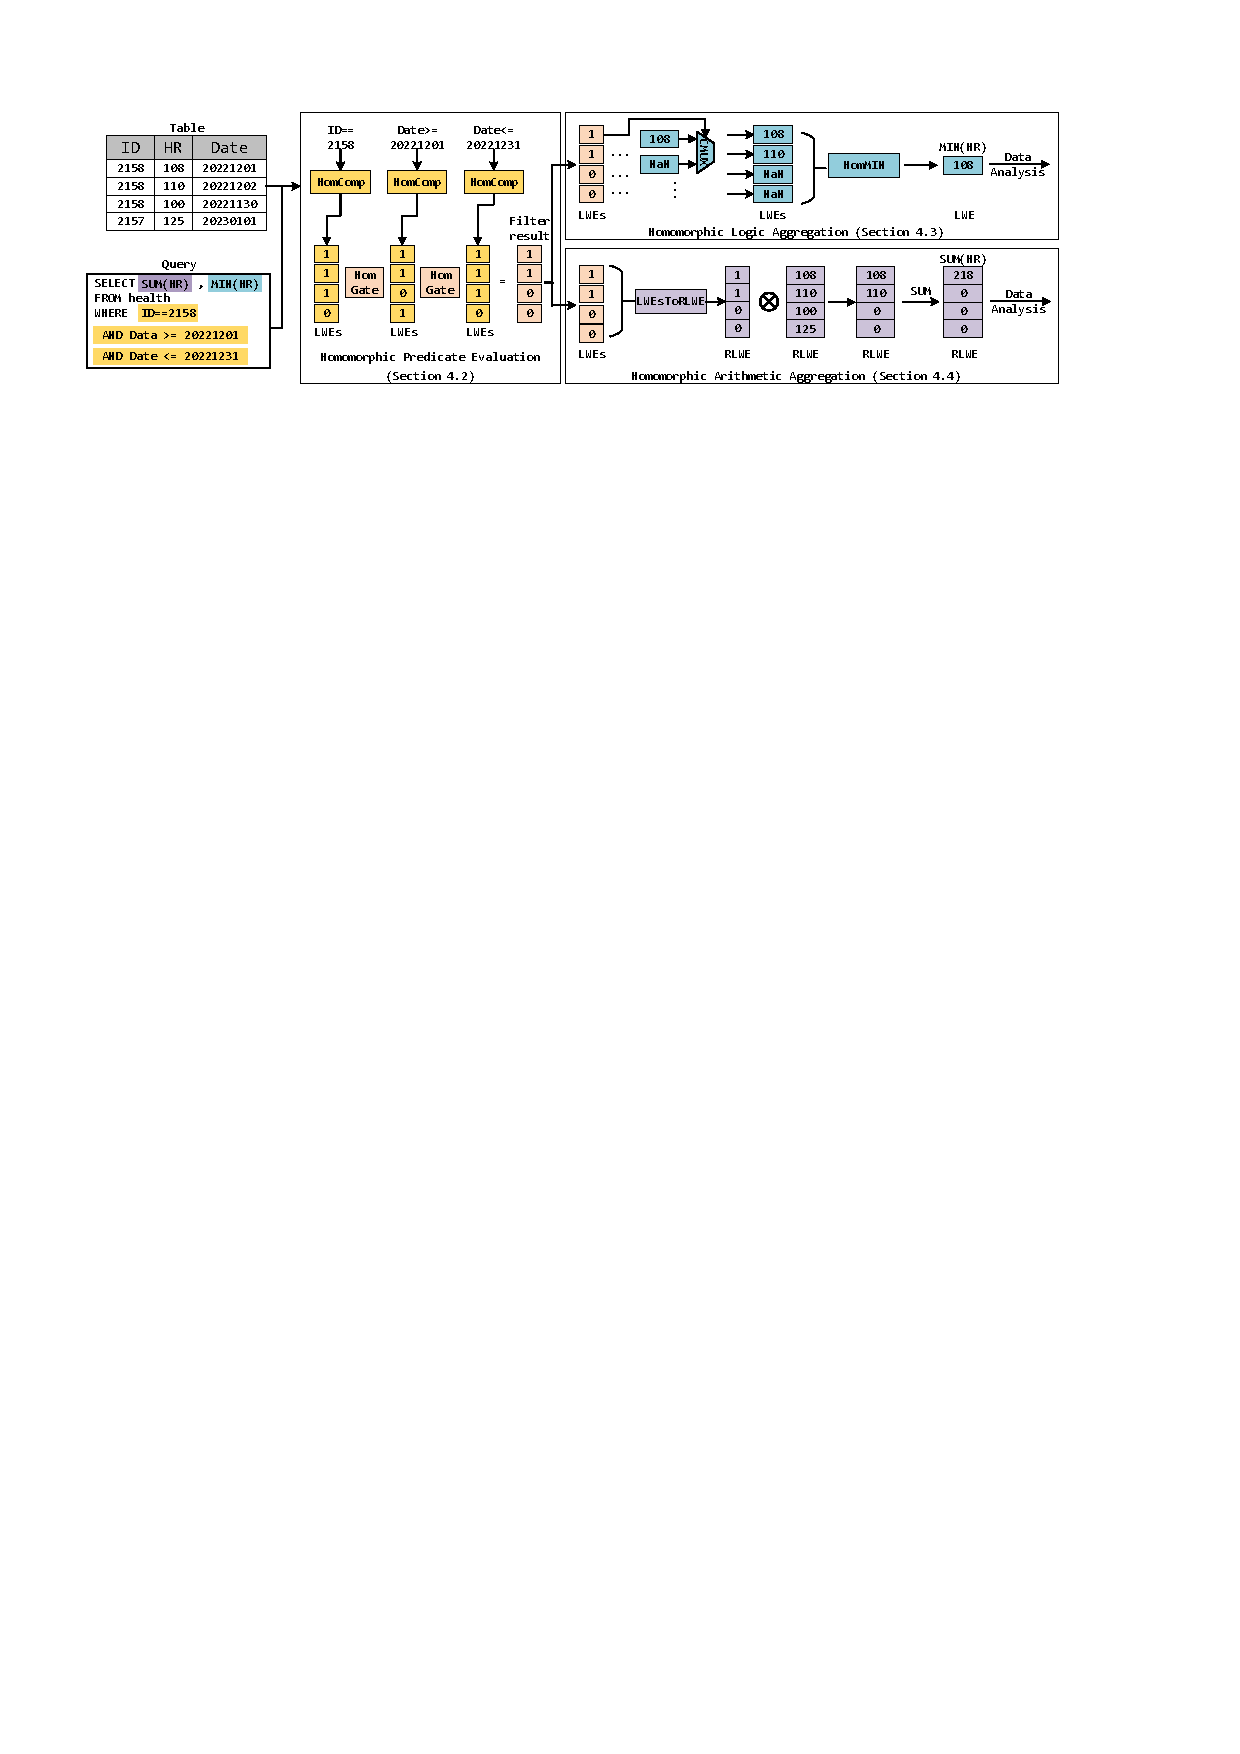
\includegraphics[width=\linewidth]{figure/query_evaluation.pdf}
%   \end{center}
%    \vspace{-0.5em}
%      \caption{sql query example.} 
%   \label{fig: sql_example}
%   \vspace{-0.5em}
%\end{figure}
%
%after the query processing, 
%the result is
%$\mathcal{r} = (r_1, ...,r_{\lvert g \rvert})$
%where $r_i$ is the aggregated value of $g_i$.
%in \cref{fig: sql_example}, $r = (r_1, r_2)$
%and $r_1$ is the value of \texttt{AVG(HR)}.

\section{Framework Overview} \label{framework}
In this section, 
% we propose our novel fully homomorphic database framework, 
% called \NAME,
% to query and process encrypted data with  
% cost-effectiveness, high elasticity, and high security.
we first provide a high-level workflow 
of \NAME in \cref{framework:workflow},
and then analyze the threat model and security guarantees of \NAME
in \cref{framework: threat_model}. Lastly, we summarize how to
implement key SQL statements for the filter-aggregation process
in \cref{block: overview}.

% briefly review the overall workflow 
% and 
% the overall architecture
% and then provide a straightforward example to illustrate the \NAME workflow.


\subsection{\NAME Workflow} \label{framework:workflow}
\begin{figure*}[t!]
   \begin{center}
   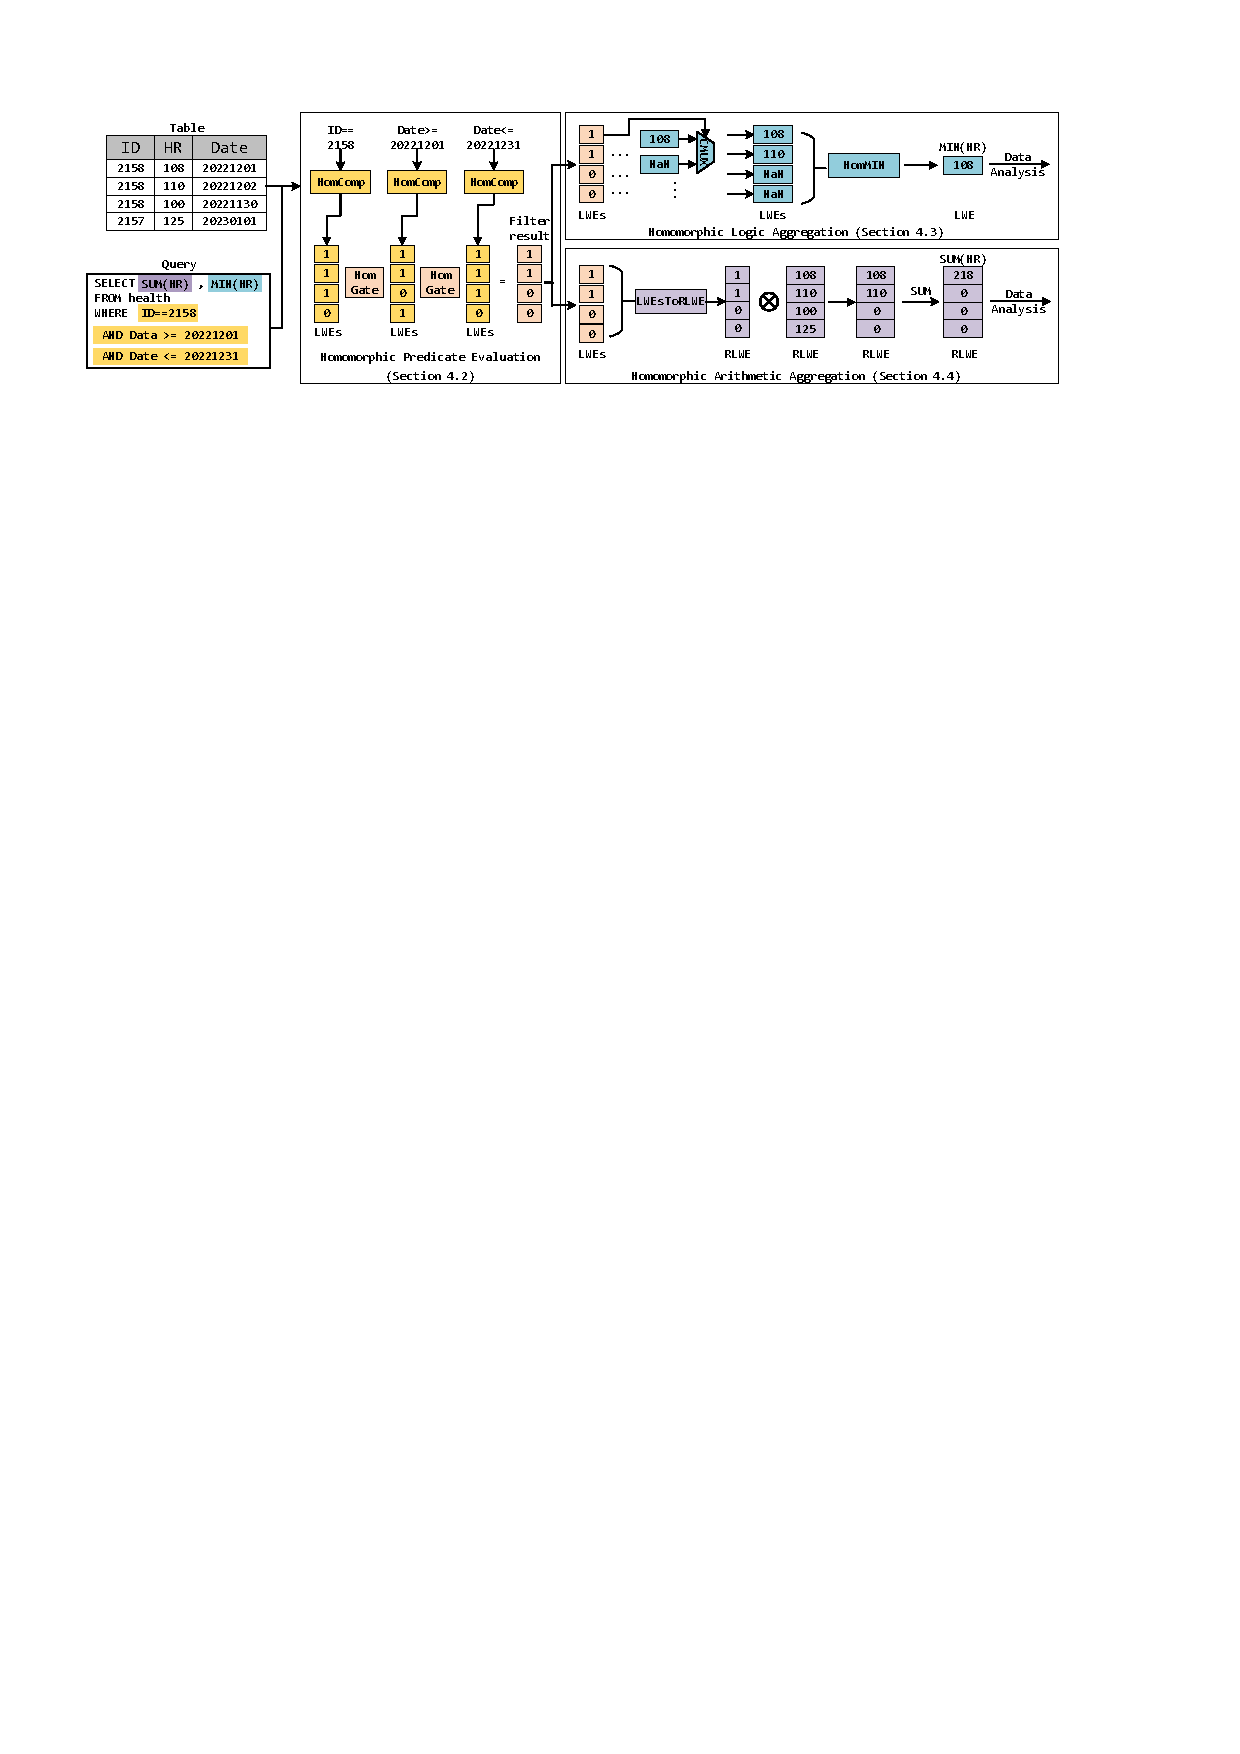
\includegraphics[width=\linewidth]{figure/query_evaluation.pdf}
   \end{center}
    % \vspace{-0.5em}
      \caption{An example processing
      flow illustration in query evaluation. Here, we show
      how to perform logic aggregation ($\hommin$) and arithmetic aggregations.
      Plaintext values in the figure are used only to demonstrate
      the range for each of the attributes.}
      \Description{A encrypted query evaluation process consists of three parts: 
      homomorphic predicate evaluation, homomorphic logic aggregation, and homomorphic
      arithmetic aggregation.}
   \label{fig: query_eva}
   % \vspace{-0.5em}
\end{figure*}
\begin{table*}[t!]
    % \footnotesize
    \centering
    \caption{Summary of Operation Costs for Each Homomorphic SQL 
    Statement.}

    % \vspace{-0.5em}
        \begin{tabular}{ccccc}
            \toprule
            SQL Statement & \#\homcomp & \#\homgate & \#\cmux & \#\cb\\
            \midrule
            $\select$ & $\dbtabrow \cdot \dbabsquery$& 
            $\dbtabrowsize \cdot (\dbabsquery - 1)$ & 0 & 0\\
            $\join$ & $\abs{\dbtab_a}_{\rm row} \cdot \abs{\dbtab_b}_{\rm row}$&
            0 & 0 & 0\\
            $\groupby$ & $\dbtabrow \cdot \abs{\attribute}$ &
            0 & 0 & 0\\
            $\orderby$ & $\dbtabrow \log_{2}^{2}{\dbtabrow } $ & 0 
            & $\dbtabrow (\log_{2}^{2}{\dbtabrow } + 1) $&
            $\dbtabrow (\log_{2}^{2}{\dbtabrow } + 1) $ \\
             $\dbmin/\dbmax$ & $\dbtabrow - 1$ & 0 & $2\dbtabrow - 1$ & $2\dbtabrow - 1$\\
            
            
            \bottomrule
        \end{tabular}\\
    \label{tab: sqlcost}
    {\footnotesize{$|\dbquery|, \dbtabrowsize$ and
    $|\attribute|$ are all public data known to the server.}}
\end{table*}
The \NAME framework is composed of three interlinked stages:
%as depicted in \cref{fig: workflow}: 
(1) offline data encryption, 
(2) online query processing, and (3) online data analysis.
In what follows, we detail the main objective of each stage and 
briefly sketch the lower-level FHE operations.

% \begin{figure*}[t!]
%     \begin{tabular}{p{0.2cm}<{\raggedright}
%     m{7cm}<{\raggedright}
%     m{2cm}<{\centering}
%     m{6.5cm}<{\raggedright}}
%     \toprule
%     & \multicolumn{1}{c}{Client} & &  \multicolumn{1}{c}{Server} \\
%     \midrule
%     \multicolumn{2}{l}{{\bf{Offline Data Encryption Stage}}} & & \\
%     1.& Set up FHE parameters and secret key. & & \\
%     2.& Initialize data $\mathcal{T} = (t_1, t_2, ..., t_{\abs{\mathcal{T}}_c})$ & &\\
%     3.& Initialize Model: $\mathcal{M} = (w_{1}, w_{2}, ..., w_{\lvert \mathcal{M} \rvert_c}, 
%     \mathcal{C})$ & & \\
%     4. & Encrypts each column of $\mathcal{T}$ using RLWE encryption
%     and gets the encrypted table: $\mathcal{CT} = 
%     (ct_1, ct_2, ..., ct_{\lvert \mathcal{T} \rvert_c})$ & 
%     $\xrightarrow{\quad\mathcal{CT}\quad}$  & Encrypted Table: $\mathcal{CT}$ \\
%     5.& Encrypts each weight of the model and
%     gets the encrypted model $\mathcal{CM} =
%     = (cw_1, cw_2, ...,cw_{\lvert \mathcal{M} \rvert_c}, \mathcal{C})$ &
%     $\xrightarrow{\quad\mathcal{CM}\quad}$ & Encrypted Model: $\mathcal{CM}$ \\
%     \midrule
%     \multicolumn{2}{l}{{\bf{Online Query Processing Stage}}} & & \\
%     4.& Initialize Query: $\mathcal{Q} = (p_{1}, p_{2}, ..., p_{\abs{\mathcal{Q}}}, B, G)$ & & \\
%     5.& Encrypts each predicate of the query and gets the encrypted query
%     $\mathcal{CQ} = 
%     (cp_{1}, cp_{2}, ..., cp_{\abs{\mathcal{Q}}}, B, G)$ & 
%     $\xrightarrow{\quad\mathcal{CQ}\quad}$ & 
%     Encrypted Query: $\mathcal{CQ}$ \\
%     6.& & & Processing $\mathcal{CQ}$ 
%     on $\mathcal{CT}$ 
%     and gets the encrypted query result 
%     $\mathcal{CR} = (cr_1, cr_2,..., cr_{\abs{G}})$ \\
%     \midrule
%     \multicolumn{2}{l}{{\bf{Online Data Analysis Stage}}} & & \\
%     10.& & & Switch the query result for data analysis
%     and gets the analysis result: $ \mathcal{CR}_{\mathcal{M}}=\mathcal{CM}(\mathcal{CR})$ \\
%     11.& Decrypts and gets the final result: $\mathcal{M}(\mathcal{R})$ & 
%     $\xleftarrow{\quad\mathcal{CR_{\mathcal{M}}}\quad}$ & Evaluation Result:  $\mathcal{CR}_{\mathcal{M}}$\\
%     \bottomrule
%     \end{tabular}
%     \caption{The workflow illustration of \NAME with three main stages: the offline data encryption stage, the online query processing stage, and the 
%     online data analysis stage. }
%     %The notation follows the definition in \cref{pre: he_db}}
%     \label{fig: workflow}
% \end{figure*}

% \textbf{(1) Offline Data Encryption Stage}: 

To begin with,  in (1) the offline data encryption stage, 
the client first needs to encrypt all the data tables in the database 
using FHE and outsources the encrypted database to the server. 
Specifically, for every table $\dbtab\in\db$, each column $t_i\in\dbtab$ 
will first be divided into $J=\lceil \dbtabrowsize/N\rceil$ data chunks,
each of size $N$. Next, 
each data chunk is encoded into a degree-$N$ plaintext polynomial $\ttm_{i, j}$, and 
encrypted into an RLWE ciphertext $\rlwe(\ttm_{i, j})$. The resulting encrypted
database is thus a set of RLWE ciphertexts $\{\rlwe(\ttm_{i, j})\}$ along
with the associated keys (i.e., $\bBK$ and $\mathbf{CK}$).
Along with the encryption database, the evaluation keys $\bBK$
will also be sent to the server.
We note that different from existing bit-by-bit~\cite{aphadb}
and row-by-row~\cite{heda} schemes, we encrypt the entire database using only RLWE
ciphertexts, significantly reducing the client-side encryption complexity and communication
burdens.
% Based on the security of the FHE ciphertexts, 
% the server could not gain any information without 
% the secret key. 
% We provide more security analysis in \cref{framework: threat_model}.


% \textbf{(2) Online Query Processing Stage}:
Next, two main steps in (2) the online query processing stage,
are homomorphic filtering and homomorphic aggregation. 
% Here, the client initiate SQL query over the outsourced data, 
% which can contain a set of particular combination of the 
% $\select$, $\join$, $\groupby$, $\orderby$, aggregation and further data analysis 
% operations. 
For filtering, we execute a number of homomorphic comparisons to
realize the $\select$, $\join$, $\groupby$, and $\orderby$ filtering 
operations on
encrypted data items, and more details on the exact input-output
behaviors of these SQL statements are provided in \cref{block: overview}. 
Then, logic 
(\texttt{MIN}, \texttt{MAX}, \texttt{Top-k})
and arithmetic (\texttt{SUM}, \texttt{AVG}) aggregations are executed
according to the statements in the queries. To better convey our idea,
we first summarize how the SQL statements are built over the proposed FHE 
operators in \cref{block: overview}. Later in \cref{block},
the proposed high-precision homomorphic comparison, aggregation,
and conversion operators are presented. % can be found in \cref{block}.
% We point out two
% main challenges here. First, it is highly non-trivial to
% efficiently evaluate a rich class of encrypted predicates with
% unbounded predicate depth and high operand precision.
% cost-effectiveness and high precision (\cref{block: comparison}).
% The server evaluates the query $\mathcal{CQ}$ 
% on the encrypted table $\mathcal{CT}$
% homomorphically.
% The processing of the encrypted query on encrypted data follows two steps: 
% The filtering period retrieves records from the table 
% according to the specified predicate from the clause,
% which contains lots of comparisons 
% as well as logic gates.
% The aggregation stage groups multiple values of 
% filtering results to 
% calculate a summary value, which consists of logical aggregations

% Although FHE could support these operations nat\"ively, 
% there still faces two main challenges. 
% The first is how to perform unbounded encrypted predicate evaluation with
% cost-effectiveness and high precision (\cref{block: comparison}).
% As the filtered result is in encrypted form, the second challenge is 
% how to evaluate homomorphic aggregations
% only on filtered rows with high precision, 
% including homomorphic logic aggregations (\cref{block: minmax})
% and homomorphic arithmetic aggregations (\cref{block: LWEsPack}).


% While the user is willing to query her data, 
% she encrypts the sensitive part (predicate value) of the query
% and sends the homomorphically encrypted query $\mathcal{CQ}$
% to the cloud server.


% \textbf{(3) Online Data Analysis}: 
If needed, the server performs further computations on 
the aggregated results in (3), the online data analysis stage.
In most practical applications, the client 
also wishes to outsource some data analysis 
algorithms. Here, we assume that
%To achieve such a goal, the user encrypts the model and sends it to the server.
the data analysis algorithm $\calgo$ contains a set of algorithm parameters  $\algoweight$,
which belongs to either the client or the server.
Unfortunately, due to the limit of 
ciphertext noise level~\cite{aphadb, heda} or incompatible plaintext encoding~\cite{sagma},
queried results produced by existing FHE-based SDO often cannot be further 
processed without additional client-server interactions.
In contrast, through the carefully designed homomorphic aggregation and conversion operators,
\NAME permits arbitrary $\calgo$ to be applied on the queried ciphertext results.
A detailed presentation for the data analysis stage can be found in \cref{Analysis}.
% data analysis methods may not achieve the best efficiency
% when dealing with aggregation results obtained from step \textbf{(2)},
% due to the unmatched ciphertext formats~\cite{sagma} or noise overflow~\cite{aphadb, heda}.
% Though, it is necessary to switch (\revise{bootstrap}) the aggregated ciphertext elastically 
% to support general data analysis (\cref{Analysis}). 

\subsection{Threat Model and Security} \label{framework: threat_model}
{\bf{Threat Model}}: Our security goal is to protect the outsourced database $\mathcal{D}$
owned by the client $\mathcal{C}$ from the semi-honest server $\mathcal{S}$,
and our threat model is similar to that in previous works\cite{cryptdb, sagma, aphadb, 
sortinghat, heda}.
% Here, the $\mathcal{C}$ encrypts the private $\mathcal{D}$
% using FHE and outsources to the $\mathcal{S}$. 
We assume that $\mathcal{S}$ honestly follows the protocol to
execute the queries and data analysis algorithms, but acts as 
a probabilistic polynomial time adversary and perform computations to 
learn as much as possible from $\db$ owned by $\mathcal{C}$.
The concrete public and private data from the perspective of the server is as follows. 
% the notation follows the definition in \cref{pre: he_db}.

\noindent {\bf{Public Data}}: 
\begin{itemize}
    \item $\abs{\mathcal{D}}$:
    the size of the database, i.e., the number of data tables in $\mathcal{D}$.
    \item $\dbtabrowsize$, $\dbtabcolsize$:
    the number of rows as well as the number of columns in some
    table $\dbtab\in\db$. 
    \item $\abs{\dbquery}$: 
    the number of filtering predicates in a SQL query $\dbquery$.
    \item $\attribute, |\attribute|$: The attribute label (e.g., gender, date)
    and the range of the attribute (e.g., $|\mathsf{Gender}|=2$).
    \item The logic connection (e.g., AND, OR) between the filtering predicates in a SQL query.
    \item The aggregation functions (e.g., $\dbsum$, $\dbmin$) in a SQL query. 
    \item $\calgo$: the data analysis algorithm without parameters (i.e., only the procedures).
\end{itemize}

\noindent {\bf{Private Data}}: %The following data need to be protected from the server.
\begin{itemize}
    \item $\mathcal{T}_{i, j}$,
    for $i \in \dbtabrowsize$, $j \in \dbtabcolsize$
    : exact values of the database items for all $\dbtab\in\db$.% i.e.,  
    \item $\mathcal{Q}_i \in \mathcal{Q}$, for $i \in \abs{\mathcal{Q}}$: 
    the predicate values in the SQL query.
    \item $w_i \in \mathcal{W}$, for $i \in \abs{\mathcal{W}}$: 
    the weight values of the data analysis algorithm $\calgo$.
\end{itemize}

{\bf{Security of \NAME}}: Since the private data are all encrypted using
FHE, the security of \NAME can be directly 
reduced to that of the underlying FHE scheme.
Traditional FHE schemes, such as B/FV~\cite{DBLP:conf/crypto/brakerski12}, CKKS~\cite{DBLP:conf/asiacrypt/CheonKKS17}, and TFHE~\cite{DBLP:journals/joc/ChillottiGGI20}, 
all guarantee security under chosen plaintext attacks, 
which translates to a semi-honest security 
on private client data.
Assuming the circular security of FHE~\cite{DBLP:conf/innovations/bgv12}, 
switching between different ciphertext formats preserves 
the overall semi-honest security of the protocol.
However, the parameters of such ciphertext formats 
need to be jointly adjusted to achieve the same level of security.
Note that, since \NAME protects both the query values
and the intermediate results, \NAME is secure
against access patterns as well as volume leakage attacks~\cite{attackSOD}.
% However, like most FHE applications, 
% the circuit privacy is out of the scope of this work.  

\subsection{Key Operators in Filter-Aggregation}\label{block: overview}
Since a SQL query can contain a variety of composed filtering and aggregation statements,
\NAME breaks each statement down to atomic operators that can be directly
implemented using FHE.
Here, we use the simple plaintext SQL query shown in \cref{fig: query_eva} as an illustration
for the statement evaluation process.
% and analyze the homomorphic operator costs for distinct SQL statements with respect 
% to the input size $\dbabstab$ in \cref{tab: sqlcost}.

$\bullet$ $\boldsymbol{\select}$. 
The homomorphic $\select$ operator takes as inputs
$\dbabsquery$ encrypted predicates with 
$\dbtabcolsize \cdot J$ $(J=\lceil \dbtabrowsize/N\rceil)$ columns of RLWE ciphertexts,
and outputs a set of LWE ciphertexts
$\mathbf{sc} = (sc_0, sc_1 ,..., sc_{\dbtabrowsize-1})$.
Here, each $sc_i$ is an LWE
ciphertext that encrypts either $1$ (true) or $0$ (false), 
indicating if the $i$-th row of $\dbtab$ is selected.
Functionally, the homomorphic $\select$ operator consists
two steps: i) individual predicate evaluation, and ii) logic
connection between the predicates.
In \NAME, encrypted predicate evaluations (as shown in \cref{fig: query_eva})
are realized as homomorphic logical comparisons ($>, \geq, <, \leq, ==, \ne$)
between ciphertexts based on the $\homcomp$ operator. Since
$\homcomp$ is one of the key building blocks for our framework, 
more discussions on $\homcomp$ are delivered in \cref{block: comparison}.
%and could be evaluated by the
Besides, the unbounded-depth logic connection (AND, OR) between the 
individual comparison results
can be implemented by the $\homgate$ operator defined in 
\cref{pre:he_circuits}. Since FHE-based filtering is inherently a
linear scan, the cost of $\homcomp$ in $\select$ is $\dbtabrowsize \cdot 
\dbabsquery$ since 
each predicate requires the comparison between the queried predicate value and
all items in the corresponding column of the encrypted table ($\dbtabrow$).
% of the certain column and  the ciphertext of the predicate value.
In addition, connecting $\dbabsquery$ predicates cost $\dbtabrow \cdot (\dbabsquery - 1)$  
$\homgate$ operations, as the $\dbabsquery$ predicates contains $(\dbabsquery - 1)$
logic connections between the individual comparison results.
% Consider an example 
% predicate \texttt{ID == 2158} in $\dbquery$,
% it requires the comparison between all the encrypted records ($\abs{\dbtab}_r$) of 
% the column \texttt{ID} and 
% the ciphertext of the predicate value \texttt{2158},
% which contains $\abs{\dbtab}_r$ homomorphic comparisons.
% Moreover, the results of $\abs{\dbquery}$ predicates
% will be integrated into the selected result by
% $\abs{\dbquery} - 1$ gate operators, while each operators handles
% $\abs{\dbtab}_r$ comparison results from homomorphic predicate evaluation.
% in \cref{block: comparison}. 

$\bullet$ $\boldsymbol{\join}$.
A homomorphic inner join is composed of 
the Cartesian product of the two encrypted tables
and the evaluation of the join condition, which can simply be 
implemented by the homomorphic comparison operator $\homcomp$.
Thus, for two data tables $\dbtab_{a}$ and $\dbtab_{b}$, 
the cost of $\homcomp$ in $\join$ is 
$\abs{\dbtab_a}_{\rm row} \cdot \abs{\dbtab_b}_{\rm row}$.

$\bullet$ $\boldsymbol{\groupby}$.
To evaluate the homomorphic $\groupby$ operator,
we generate multiple copies of the original query $\dbquery$, 
where each copy is equipped with an additional equality test over the group 
attribute. For example, a $\groupby$ on the attribute $\mathsf{Gender = \{0,1\}}$ 
can be implemented by the two queries $\dbquery\text{ } \reg{AND} \text{ }\mathsf{Gender == 0}$
and $\dbquery\text{ } \reg{AND} \text{ }\mathsf{Gender == 1}$.
Let the range of the $\groupby$ attribute $\attribute$ be $\abs{\attribute}$,
the cost of $\groupby$ is $\dbtabrow \cdot \abs{\attribute}$ $\homcomp$ operations.

$\bullet$ \textbf{Aggregation functions}.
As shown in \cref{fig: query_eva},
after the homomorphic predicate evaluation, 
we get $\dbtabrowsize$
LWE ciphertexts encrypting the filtering results.
The homomorphic aggregation computes the functions
on the filtered rows.
\NAME supports both logic aggregation 
(such as $\dbmin, \dbmax$, and $\dbtopk$)
and arithmetic aggregation 
(such as $\dbsum, \dbavg$, and $\dbcount$) functions,
and we detail the exact constructions in \cref{block: minmax} and \cref{block: LWEsPack}.
%$\bullet$ $\boldsymbol{\orderby}$.
Additionally,  we note that, $\orderby$ is
essentially a logic aggregation, and can be implemented similar to
$\dbtopk$.
% homomorphic comparison $\homcomp$ and homomorphic selector $\cmux$.
The main challenge for all types of homomorphic logic aggregations is how to apply 
numerical comparisons
only on the filtered result. Since a logic mismatch is represented
using a value 0 in most existing homomorphic comparison 
operators~\cite{pegasus,sortinghat},  comparing
logic mismatches and legitimate attribute values may produce incorrect aggregation 
results. 
We detail our method to overcome this challenge in \cref{block: minmax}.
%\input{ccs-body/framework/threat_model.tex}
\section{Cryptographic Building Blocks}\label{block}


In this section, 
% we present the homomorphic query evaluation algorithm for 
%we detail the online query processing stage in \NAME.
% We briefly review the SQL statements in \NAME
% and provide a plaintext illustration in \cref{block: overview}.
we introduce the main cryptographic tools we develop,
namely, the homomorphic comparison operator $\homcomp$ for
homomorphic predicate evaluation (\cref{block: comparison}), 
the homomorphic minimum and maximum operators 
$\hommin$ and $\hommax$
for homomorphic logic aggregation (\cref{block: minmax}),
%\texttt{MIN/MAX}, 
and a new $\repack$ operator for homomorphic arithmetic aggregation  
(\cref{block: LWEsPack}).

% to 
% significantly enhance the computational performance
% and digital precision in 

% These three algorithms are also of 
% independent interest in the FHE research community.



% \subsection{Overview}\label{block: overview}
% \begin{table*}[t!]
%     % \footnotesize
%     \centering
%     \caption{Summary of operation costs for homomorphic SQL operators.
%     Here, the $\dbtabrow$ stands for the number of rows in the table 
%     $\dbtab$, the $\abs{\attribute}$ represents the range of 
%     attribute.}
%     \vspace{-0.5em}
%         \begin{tabular}{ccccc}
%             \toprule
%             operator & \#\homcomp & \#\homgate & \#\cmux & \#\cb\\
%             \midrule
%             $\select$ & $\dbtabrow \cdot \dbabsquery$& 
%             $\abs{\dbtab}_r \cdot (\dbabsquery - 1)$ & 0 & 0\\
%             $\join$ & $\abs{\dbtab_a}_c \cdot \abs{\dbtab_b}_c$&
%             0 & 0 & 0\\
%             $\groupby$ & $\dbtabrow \cdot \abs{\attribute}$ &
%             0 & 0 & 0\\
%             $\orderby$ & $\dbtabrow \log_{2}^{2}{\dbtabrow } $ & 0 
%             & $\dbtabrow (\log_{2}^{2}{\dbtabrow } + 1) $&
%             $\dbtabrow (\log_{2}^{2}{\dbtabrow } + 1) $ \\
%              $\dbmin/\dbmax$ & $\dbtabrow - 1$ & 0 & $2\dbtabrow - 1$ & $2\dbtabrow - 1$\\
%             
%             
%             \bottomrule
%         \end{tabular}
%     \label{tab: sqlcost}
% \end{table*}
% 
% In this section, we talk about how \NAME supports SQL query
% operators including $\select, \join, \groupby, \orderby$
% , and aggregation functions. 
% We provide a simple plaintext illustration in \cref{fig: query_eva}
% and analyze the homomorphic operator costs for distinct SQL statements with respect to the input size $\dbabstab$ in \cref{tab: sqlcost}.
% 
% $\bullet$ $\boldsymbol{\select}$. 
% The homomorphic $\select$ operator inputs 
% $\dbabsquery$ encrypted predicates with 
% $\dbtabcolumn$ columns of RLWE ciphertexts
% and outputs a set of LWE ciphertexts
% $\mathbf{sc} = (sc_0, sc_1 ,..., sc_{\dbtabrow-1})$
% where each $sc_i$ is an LWE
% ciphertext which encrypts $1$ or $0$, 
% indicating the $i$-th row of $\dbtab$
% is selected or not.
% The homomorphic $\select$ operator contains 
% the homomorphic predicate evaluation and the gate operation
% between the predicate results.
% In \NAME, 
% the encrypted predicate (as shown in \cref{fig: query_eva})
% is the logical comparison 
% ($>, \geq, <, \leq, ==, \ne$)
% between 
% two ciphertexts
% and could be evaluated by the
% homomorphic comparison $\homcomp$ operator in \cref{block: comparison}.
% The gate operation (AND, OR)
% between the comparison results
% could be implemented by the $\homgate$ defined in 
% \cref{pre:he_circuits}.
% The cost of $\homcomp$ in $\select$ is $\dbtabrow \cdot 
% \dbabsquery$ since 
% each predicate requires the comparison between all the encrypted records ($\dbtabrow$) of 
% the certain column and 
% the ciphertext of the predicate value.
% And the cost of $\homgate$ in $\select$ is $\dbtabrow \cdot (\dbabsquery - 1)$  
% as the $\dbabsquery$ predicates contains $(\dbabsquery - 1)$
% gate operators applied to the results of the comparison.
% % Consider an example 
% % predicate \texttt{ID == 2158} in $\dbquery$,
% % it requires the comparison between all the encrypted records ($\abs{\dbtab}_r$) of 
% % the column \texttt{ID} and 
% % the ciphertext of the predicate value \texttt{2158},
% % which contains $\abs{\dbtab}_r$ homomorphic comparisons.
% % Moreover, the results of $\abs{\dbquery}$ predicates
% % will be integrated into the selected result by
% % $\abs{\dbquery} - 1$ gate operators, while each operators handles
% % $\abs{\dbtab}_r$ comparison results from homomorphic predicate evaluation.
% % in \cref{block: comparison}. 
% 
% $\bullet$ $\boldsymbol{\join}$.
% A homomorphic inner join is composed of 
% the Cartesian product of the two encrypted tables
% and the evaluation of the join condition, which could be 
% implemented by homomorphic comparison operator $\homcomp$.
% Thus, the cost of  $\homcomp$ in $\join$ is 
% $\abs{\dbtab_a}_c \cdot \abs{\dbtab_b}_c$.
% 
% $\bullet$ $\boldsymbol{\groupby}$.
% To evaluate the homomorphic $\groupby$ operator,
% we segregate the original query $\dbquery$ into several queries, 
% each with additional equality comparison predicates.
% For example, $\groupby$ the attribute $\mathsf{Sex = \{0,1\}}$ 
% could be implemented by $\dbquery$ with additional predicate $\mathsf{Sex = 0}$
% and $\dbquery$ with additional predicate predicate $\mathsf{Sex = 1}$.
% Supposing the range of $\groupby$ attribute $\attribute$ is $\abs{\attribute}$.
% Thus, the cost of  $\homcomp$ in $\groupby$ is 
% $\dbtabrow \cdot \abs{\attribute}$.
% 
% $\bullet$ $\boldsymbol{\orderby}$.
% The homomorphic $\orderby$ operator could be implemented by
% homomorphic comparison $\homcomp$ and homomorphic selector $\cmux$.
% The main challenge is how to only sort the selected encrypted records. 
% We detail our method to overcome this challenge \cref{block: minmax}.
% 
% $\bullet$ \textbf{Aggregation functions}.
% As shown in \cref{fig: query_eva},
% after the homomorphic predicate evaluation, 
% we get $\abs{\mathcal{T}}_{r}$
% LWE ciphertexts encrypt the filtering results.
% The homomorphic aggregation computes the functions
% on the filtered rows.
% \NAME supports both logic aggregation 
% (such as $\dbmin, \dbmax$, and $\dbtopk$)
% and arithmetic aggregation functions
% (such as $\dbsum, \dbavg$, and $\dbcount$).
% We detail the exact method in \cref{block: minmax} and \cref{block: LWEsPack}.
% As shown in \cref{fig: query_eva}, to calculate \texttt{MIN(HR)}, 
% we first selected the satisfied rows and perform \texttt{HomMIN} operations.}

% \revise{\cref{fig: query_eva} illustrate a plaintext process 
% of query evaluation in \NAME.
% It works on the encrypted table $\mathcal{CT}$, that is, 
% a set of RLWE ciphertexts 
% $(ct_1, ct_2, ..., ct_{\lvert \mathcal{T} \rvert_{c}})$.
% On a high level, the evaluation of encrypted query 
% $\mathcal{CQ} = (cp_{1}, cp_{2}, ... ,cp_{\lvert \mathcal{Q} \rvert}, B, G)$ 
% on $\mathcal{CT}$  
% can be summarized in the following steps:}

% \revise{\textbf{1) homomorphic predicate evaluation}: 
% For each encrypted predicate 
% $cp_i \in \mathcal{CQ}, i \in (1, 2, ..., \abs{\mathcal{Q}})$,
% we take the matched encrypted column ciphertext 
% $ct_d \in \mathcal{CT}$ and the predicate value ciphertext $cp_i$, 
% which are two RLWE ciphertexts, 
% to perform \texttt{HomCom} operations 
% and get a set of LWE ciphertexts $\mathbf{ctp_i}$ 
% where the $j$-th LWE ciphertext of $\mathbf{ctp_i}$ indicates 
% the $j$-th row of the table is satisfied the predicate $cp_i$ or not.
% Then we calculate the \texttt{HomGate} 
% between each comparison result $\mathbf{ctp_i}$.
% After the evaluation, we obtain a set of LWE ciphertexts 
% $\mathbf{fr} = (fr_1, fr_2 ,..., fr_{\abs{\mathcal{T}}_r})$
% where each $fr_i$ is an LWE
% ciphertext which encrypts $1$ or $0$, 
% indicating the $i$-th row of $\mathcal{T}$
% is selected or not.}
% $\mathbf{}$
% to perform
% The homomorphic predicate evaluation of $\mathcal{CQ}$
% consists of the homomorphic comparison \texttt{HomComp} in each
% predicate $cp_i$ and the homomorphic gate \texttt{HomGate} 
% between predicates.
% \revise{Gate Tree..., add an algorithm, and complexity analysis...}
 
% $i \in (1, 2, ..., \abs{\mathcal{Q}})$ in $\mathcal{CQ}$, 
% we first get the attribute index of the predicate $d$ 
% and the comparison operator $op$
% ($\geq, \leq, ==, >, <$) of the predicate.
% Here, the $ct_d$ represents the RLWE ciphertext which
% encrypts the matching column in $\mathcal{T}$
% and the $cp_i$ refers to the RLWE ciphertext of the predicate value.
% Then, we sample extract the RLWE ciphertexts $ct_d$ and $cp_i$, 
% and get two LWE ciphertext vectors
% $\mathbf{ct_d}$ and $\mathbf{cp_i}$ wich size $\abs{\mathcal{T}}_{r}$.
% For each LWE ciphertext $ct_d[j]$and $cp_i[j]$, 
% we perform \texttt{HomCom} of the two LWE ciphertext
% with the comparison operator $op$
% and get the encrypted comparison result $comp_{i,j}$.
% Next, we evaluate the logic gate between different predicates 
% using \texttt{HomGate}.


% \revise{\textbf{2) homomorphic logic aggregation}:
% After the homomorphic predicate evaluation, 
% we get $\abs{\mathcal{T}}_{r}$
% LWE ciphertexts encrypt the filtering results.
% The homomorphic logic aggregation computes the logic function
% (such as \texttt{MIN/MAX}, \texttt{Top-k})
% on the filtered rows.
% As shown in \cref{fig: query_eva}, to calculate \texttt{MIN(HR)}, 
% we first selected the satisfied rows and perform \texttt{HomMIN} operations.}
% % the \texttt{HomMIN}
% % The $\texttt{LWEsPack}$
% % packs $\abs{\mathcal{T}}_{r}$ into a RLWE ciphertext $fl$
% % for latter homomorphic aggregation.

% \revise{\textbf{3) homomorphic arithmetic aggregation}:
% The aggregation process computes the arithmetic function
% (such as \texttt{SUM}, \texttt{AVG}, and \texttt{COUNT})
% on the filtered rows.
% As the filtered result format (LWE ciphertexts) is inefficient
% to homomorphic arithmetic function.
% We need to perform homomorphic ciphertext conversion 
% \texttt{HomConvert} to pack LWE ciphertexts into an RLWE ciphertext
% for latter operators.}
% For each aggregation filed $g_i$, 
% we get the attribute index $d = g(a)_i$
% and the aggregation function $f_i = g(f)_i$.
% As the filtering result $fl$ is in coefficient format, 
% we directly perform the aggregate function when $f_i$ supports 
% coefficient format computation.
% Otherwise, we first evaluate the \texttt{CoeffToSlot} 
% to convert $fl$ to $\hat{fl}$ slot format ciphertext $\hat{fl}$
% and then computes the $f_i$ in slot format.




\subsection{Homomorphic Predicate Evaluation}\label{block: comparison}
% ckks filtering method limitation
Since predicate evaluations are essentially concatenated comparisons,
the core computation here
is the comparison between two encrypted ciphertexts.
In this section,  we outline a series of homomorphic algorithms we devised
that lead to the proposed homomorphic comparison algorithm 
$\homcomp$, which supports unbounded-depth homomorphic predicate evaluation. % and then describe 
% \revise{how it supports 
% efficient and unbounded predicate evaluation.}

\subsubsection{The Main Building Block: $\hmsb$}
We first discuss the homomorphic most significant bit (MSB) extraction algorithm, $\hmsb$, 
which is the key building block in instantiating $\homcomp$.
We first point out that, as observed in the existing works~\cite{heda, pegasus,largeprecision}, 
the comparison between two ciphertexts $ct_a$ and $ct_b$ encrypting integers $a$ and $b$
can be evaluated by extracting the MSB from $ct_a-ct_b$,
% For instance, to evaluate $a \geq b$, we compute $a -b$ and homomorphically
% extract the MSB of the reduction result. 
since the MSB of the subtraction result encrypts a value of $0$ when $a \geq b$ and 
a value of $1$ when $a \textless b$. 
However, we observe that existing homomorphic MSB extraction algorithms following the $\pbs$ 
procedure~\cite{pegasus} proposed  in~\cite{DBLP:conf/asiacrypt/tfhepbs}
may not fit encrypted databases due to their low accuracy. In particular, such algorithms
can only successfully extract the MSB when the plaintext message (which is the
subtraction result $a-b$ here)
is an integer that is less than 6 bits (the full $\pbs$-based MSB extraction algorithm can be
found in the Appendix).
%We detail the algorithm in \cref{algo: kHMSB}.
% with 
% a MSB extraction function $\msb(x) = x \geq 0 ?$ $ 0 : 1$
% is limited to small precision (less than 6 bits). 
% The main obstacle is that the precision of PBS is strictly 
% related to the parameters of the test vector 
% as we mentioned in ...
% In order to obtain high precision, one adopts a test vector with a larger
% degree or represents a high-bit ciphertext with several low-bit ciphertexts, 
% which results in an increased computation cost or storage consumption.

% {\bf{Arbitrary Precision $\hmsb$}}: 
To overcome the precision loss problem while retaining high performance,
we propose a new homomorphic MSB extraction algorithm $\hmsb$.
% to overcome the above precision loss problem.
% To overcome this, we propose our innovative method to overcome
% the tussle between latency and precision
% In this section, we propose our novel homomorphic comparison algorithm
% \texttt{HomCom} where both the inputs are ciphertexts.
% {\bf{Key Technique}}: 
% convert a high-precision comparison to 
% a low-precision comparison by iterating PBS. 
The key idea of $\hmsb$ is to iterate the $\pbs$ algorithm
a certain number of times over the same ciphertext, such that we can
extract the MSB of arbitrary-precision messages. 
% and construct arbitrary precision homomorphic MSB extraction algorithm
% by iterating $\pbs$ and $k+1$-bit $\hmsb$.
% Then we utilize the arbitrary precision $\hmsb$ to implement 
% arbitrary precision homomorphic comparisons algorithm $\homcomp$.
% Our critical insight is that, in principle, the output of 
% homomorphic MSB extraction depends only on the first bit 
% of the plaintext, so we can homomorphically \textit{discard}
% the invalid bits and consider the result as low-precision 
% ciphertext with a larger scale. In \cref{algo: 2kHMSB}, we detail the exact 
% algorithm for constructing a $2k$-bit MSB extraction using
% $(k+1)$-bit MSB extractions and PBS.

%\subsubsection{Our solution via discarding invalid bit}



% {\bf{The Base Algorithm}}: We start with a standard homomorphic MSB extraction algorithm $\hmsb_{k+1}$ 
% by initializing a $\pbs$ operator with the MSB extraction function.
% % Pegasus~\cite{pegasus} and HEDA~\cite{heda} 
% to homomorphically extract the MSB of a $k+1$-bit ciphertext. 
% % In \cref{algo: kHMSB}, it can be seen that the standard 
% % MSB extraction algorithm basically follows the PBS procedure 
% % and the precision is limited due to the degree of the test vector.
% The $\hmsb_{k+1}$ operator basically follows the PBS procedure 
% and the precision is limited due to the degree of the test vector.
% We detail the exact algorithm in \cref{algo: kHMSB}.

\begin{algorithm}[t!]
    % \tiny
    \caption{$2k$-bit $\hmsb$}
    \label{algo: 2kHMSB}
    \SetKwInOut{Input}{Input}\SetKwInOut{Output}{Output}\SetKwInOut{Return}{Return}\SetKwComment{Comment}{$\triangleright$\ }{}
    \Input{A LWE ciphertext $ct_{I} = \lwe(m)$, where $m=2^{k}\cdot m_1 + m_0$.}
    \Input{A bootstrapping key $\bBK$.}
    \Output{A LWE ciphertext $ct_{O} = \lwe(\msb(m))$.}
    $ct_{1} \leftarrow 2^{k-1}ct_{I}$ 
    \Comment*[r]{$ct_{1} = \lwe(2^{2k-1}\lsb(m_1) + 2^{k-1}m_0)$} 
    $ct_{2} \leftarrow \hmsb_{k+1}(ct_{1}) $ 
    \Comment*[r]{$ct_{2} = \lwe(2^{2k-1}\lsb(m_{1}))$} 
    $ct_{3} \leftarrow ct_{1} - ct_{2}$ 
    \Comment*[r]{$ct_{3} = \lwe(2^{k-1}m_0)$} 
    $ct_{4} \leftarrow \pbs(ct_{3}, \bBK, T(x) = \frac{x}{2^{k-1}})$ 
    \Comment*[r]{$ct_{4} = \lwe(m_0)$} 
    $ct_{5} \leftarrow ct_{I} - ct_{4}$ 
    \Comment*[r]{$ct_{5} = \lwe(2^{k}m_1)$} 
    $ct_{O} \leftarrow \hmsb_{k}(ct_{5})$
    \Comment*[r]{$ct_{O} = \lwe(\msb(m))$} 
    \Return{$ct_{O} = \lwe(\msb(m))$}
\end{algorithm}

\begin{figure}[t!]
   \begin{center}
   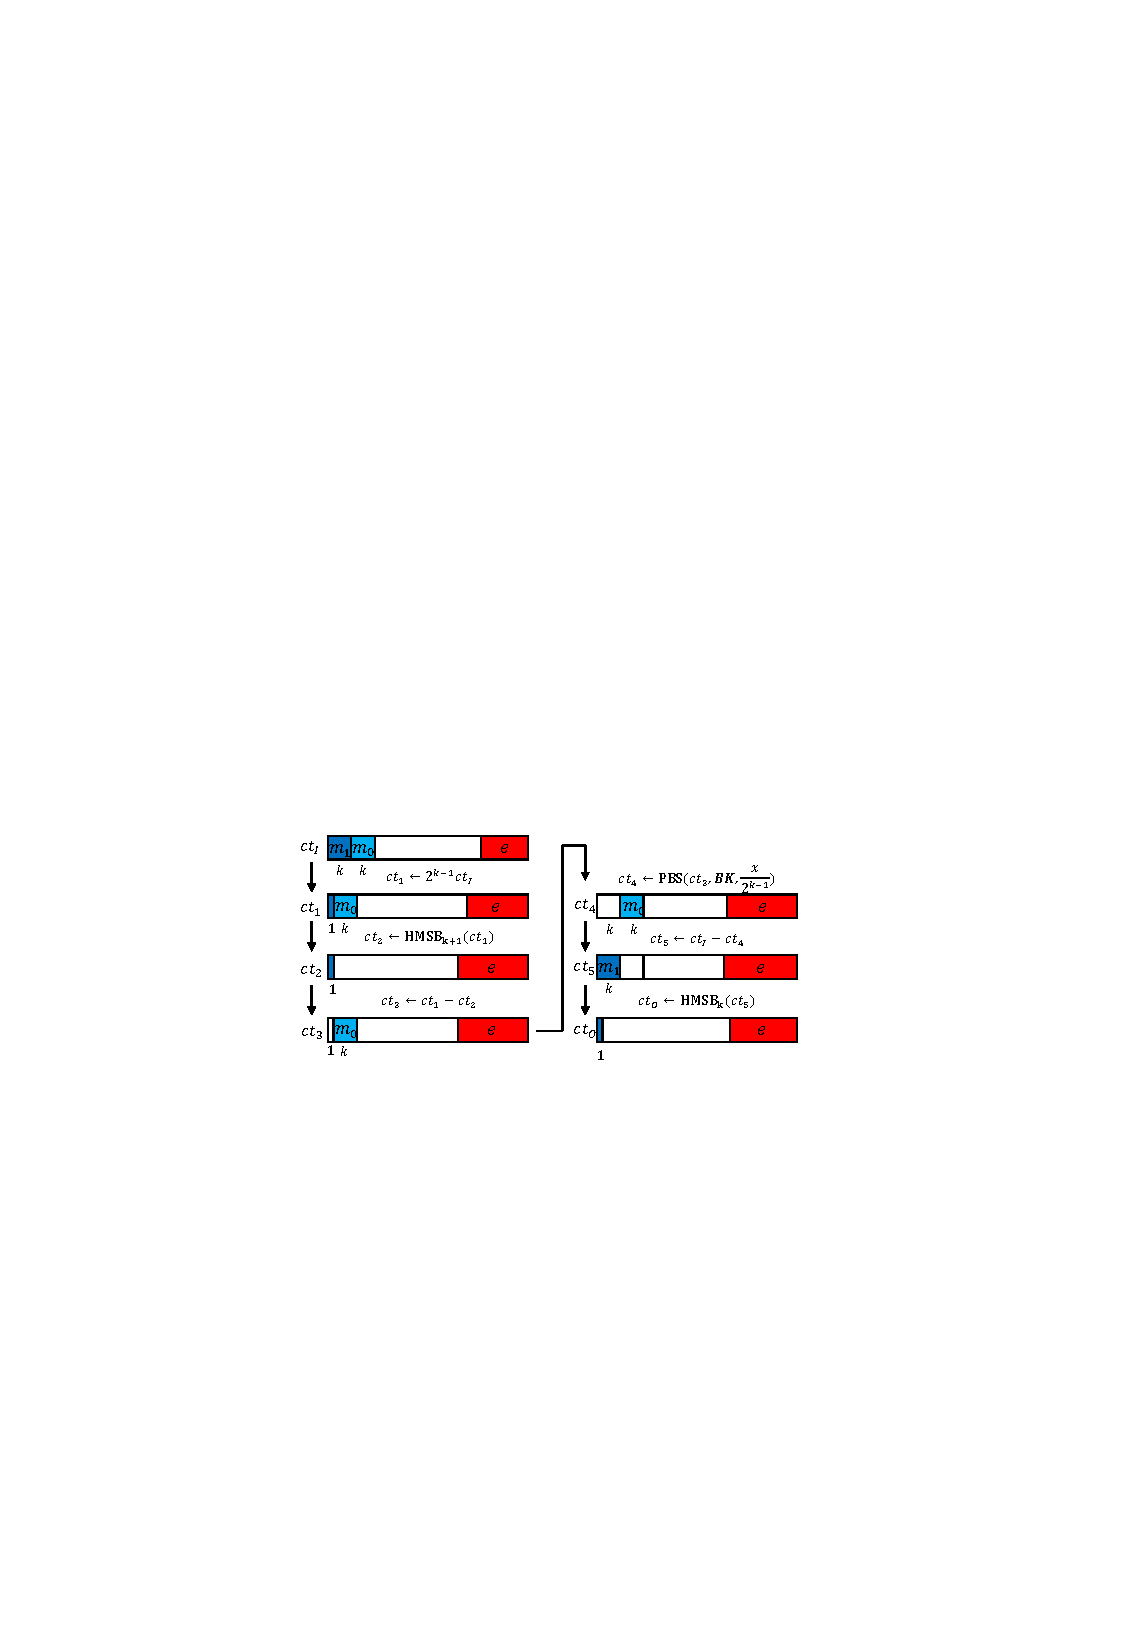
\includegraphics[width=\linewidth]{figure/hmsb.pdf}
   \end{center}
    % \vspace{-0.5em}
      \caption{A line-by-line illustration
      of how \cref{algo: 2kHMSB} works 
      with the input ciphertext $ct_{I}=\rlwe(2^{k}m_1+m_0)$.} 
      \Description{Figure 3. Fully described in the Algorithm 1}
   \label{fig: comparison}
   % \vspace{-0.5em}
\end{figure}

\begin{algorithm}[t!]
    % \tiny
    \caption{$tk$-bit $\hmsb$}
    \label{algo: tkHMSB}
    \SetKwInOut{Input}{Input}\SetKwInOut{Output}{Output}\SetKwInOut{Return}{Return}\SetKwComment{Comment}{$\triangleright$\ }{}
    \Input{A LWE ciphertext $ct_{I} = \lwe(m)$, where 
    $m=\sum_{i = 0}^{t}2^{ik} \cdot m_{i}$.}
    \Input{A bootstrapping key $\bBK$.}
    \Output{A LWE ciphertext $ct_{O} = \lwe(\msb(m))$.}
    \eIf{$t == 1$}
    {
        $ct_{O} \leftarrow \hmsb_{k}(ct_{I})$ \\
    }
    {
        $ct_{1} \leftarrow 2^{tk-1}ct_{I}$ \\
        % \Comment*[r]{$ct_{1} = {\rm LWE}(2^{(t+1)k-1}{\rm LSB}(m_1) + 2^{tk-1}m_0)$} \\
        $ct_{2} \leftarrow \hmsb_{k+1}(ct_{1}) $ \\
        % \Comment*[r]{$ct_{2} = {\rm LWE}(2^{(t+1)k-1}{\rm LSB}(m_{1}))$} \\
        $ct_{3} \leftarrow ct_{1} - ct_{2}$ \\
        % \Comment*[r]{$ct_{3} = {\rm LWE}(2^{tk-1}m_0)$} \\
        $ct_{4} \leftarrow \pbs(ct_{3}, \bBK, T(x) = \frac{x}{2^{tk-1}})$  \\
        % \Comment*[r]{$ct_{4} = {\rm LWE}(m_0)$} \\
        $ct_{5} \leftarrow ct_{I} - ct_{4}$  \\
        % \Comment*[r]{$ct_{5} = {\rm LWE}(m-m_{0})$} \\
        $ct_{O} \leftarrow \hmsb_{tk}(ct_{5})$ \\
        % \Comment*[r]{$ct_{O} = {\rm LWE}({\rm MSB}(m))$} \\
    }
    \Return{$ct_{O} = \lwe(\msb(m))$}
\end{algorithm}

We start with a $\pbs$-based MSB extraction algorithm, named $\pbshmsb$. 
We assume that $\pbshmsb$ can successfully extract the MSB of a $\kappa$-bit integer 
(e.g., as mentioned, $\kappa=6$ using the original $\pbs$ method
proposed in~\cite{DBLP:conf/asiacrypt/tfhepbs}).
Let $k=\kappa-1$ (e.g., $k=5$ in our implementation), 
we show how to construct a $2k$-bit homomorphic
MSB extraction algorithm based on $\pbshmsb$ in \cref{algo: 2kHMSB}.
First, given a $2k$-bit input ciphertext 
$ct_{I} = \lwe(m)$, it is obvious that $m=2^{k}\cdot m_1 + m_0$. 
Our critical insight is that the MSB
of $ct_{I}$ depends only on the first bit 
of the plaintext, so we can homomorphically remove
the remaining bits to construct a $k$-bit ciphertext.
% the invalid bits and consider the result as low-precision 
% ciphertext with a larger scale.
To achieve the bit removal, as depicted in \cref{fig: comparison},
we homomorphically shift the internal
plaintext message towards the left, which turns $\lwe(2^k \cdot m_1+m_0)$ 
into $\lwe(m_0)$. Next, we can homomorphically
subtract $\lwe(m_0)$ from $\lwe(m)=\lwe(2^k\cdot m_1+m_0)$, and get $\lwe(2^k\cdot m_1)$.
%to get a $k$-bit ciphertext $\lwe(2^k \cdot m_1)$.
Then, we can simply apply $\pbshmsb$ to extract the MSB of the $k$-bit plaintext message 
$m_1$, which is also the MSB of $\lwe(m)$, i.e., $ct_{I}$.
%However, to correctly
%bootstrap a ciphertext~\cite{pegasus, DBLP:conf/asiacrypt/tfhepbs}, 
%the MSB of the encrypted plaintext needs to be set to zero.
%To address this problem, we should keep one bit in the shifting processing 
%and zero it.

Based on a similar idea, we can extend the $2k$-bit
$\hmsb$ to arbitrary precision $tk$ for any positive integer $t$ by repeatedly 
shifting and subtracting $k$-bit plaintext messages. As formalized in \cref{algo: tkHMSB},
we first recursively discard the least significant $k$ bits of the initial $tk$-bit ciphertext
$t$ times until only the most significant $k$ bits remain. Then, we simply apply 
$\pbshmsb$ with $\kappa$-bit precision and accurately extract the MSB of the input
ciphertext with $tk$-bit-precision plaintext message.
%existing low-precision homomorphically MSB extraction methods~\cite{pegasus, heda}.

% By applying ${\rm HMSB}_{k+1}$ to $ct_{1}$, we get 
% $ct_{2} = {\rm LWE}_{n,q}(2^{2k-1}{\rm LSB}(m_{1}))$, which
% encrypts the LSB of $m_{1}$. 
% Then, we substract $ct_{2}$ from $ct_{1}$ and get $ct_{3}$ where 
% $ct_{3}$ which encrypts $2^{k-1}m_{0}$. After steps 2 and 3, we 
% have discarded the MSB of the encrypted plaintext and we can apply 
% PBS to $ct_{3}$. 
% and get $ct_{1}$
% . After the shifting process, 
% the most $(k-1)$bits of $m_{1}$ have been 
% moved as shown in \cref{fig: comparison}. 
% However, to correctly
% bootstrap a ciphertext, the MSB of the encrypted plaintext needs to be set to zero.
% To address this problem, we should remove the MSB of plaintext.
% By applying ${\rm HMSB}_{k+1}$ to $ct_{1}$, we get 
% $ct_{2} = {\rm LWE}_{n,q}(2^{2k-1}{\rm LSB}(m_{1}))$, which
% encrypts the LSB of $m_{1}$. 
% Then, we substract $ct_{2}$ from $ct_{1}$ and get $ct_{3}$ where 
% $ct_{3}$ which encrypts $2^{k-1}m_{0}$. After steps 2 and 3, we 
% have discarded the MSB of the encrypted plaintext and we can apply 
% PBS to $ct_{3}$. By applying PBS to $ct_{3}$, we get $ct_{4} = {\rm LWE}_{n,q}(m_0)$. And then, computing $ct_{I} - ct_{4}$, we get 
% $ct_{5} = {\rm LWE}_{n,q}(2^{k}m_1)$. Until now we have removed the 
% least $k$ bits of $m$. Finally, by applying ${\rm HMSB}_{k}$ 
% to $ct_{5}$, we obtain $ct_{O} = {\rm LWE}_{n,q}({\rm MSB}(m))$.

% \begin{algorithm}[t!]
%     % \tiny
%     \caption{$k$-bit \texttt{HMSB}}
%     \label{algo: kHMSB}
%     \SetKwInOut{Input}{Input}\SetKwInOut{Output}{Output}\SetKwInOut{Return}{Return}
%     \Input{A LWE ciphertext $ct_{I} = {\rm LWE}^{n,q}_{\mathbf{s}}(m) 
%     = (b, \mathbf{a})$, where $m \ in [0, 2^{k} -1]$.}
%     \Input{A constant $\mu = q / 4$.}
%     \Input{A bootstrapping key $\mathbf{BK}$, where 
%     $\mathbf{BK}\left[i\right] = \reg{RGSW}^{N,q}_{\Tilde{s}}(\mathbf{s}[i])$, for $i \in [1,n]$}
%     \Output{A LWE ciphertext $ct_{O} = {\rm LWE}_{\mathbf{s}}^{n,q}({\rm MSB}(m))$.}
%     % $b \leftarrow \lfloor \frac{2N}{q}b \rceil$ 
%     % and $\mathbf{a} \leftarrow \lfloor \frac{2N}{q}\mathbf{a} \rceil$ \\
%     $\Tilde{v} \leftarrow \mu \cdot (1 + x^2 + x^3 + ... + x^{N-1}) $ \\
%     $ACC \leftarrow \texttt{BlindRotate}(\Tilde{v}, ct_I, \mathbf{BK})$ \\
%     $ct_{O} = (b', \mathbf{a'}) = \texttt{SampleExtract}(ACC)[0]$ \\
%     \Return{$ct_{O} = (b' + \mu, \mathbf{a}) 
%     = {\rm LWE}_{\mathbf{s}}^{n,q}({\rm MSB}(m))$}
% \end{algorithm}



% \begin{figure*}[t!]
%    \begin{center}
%    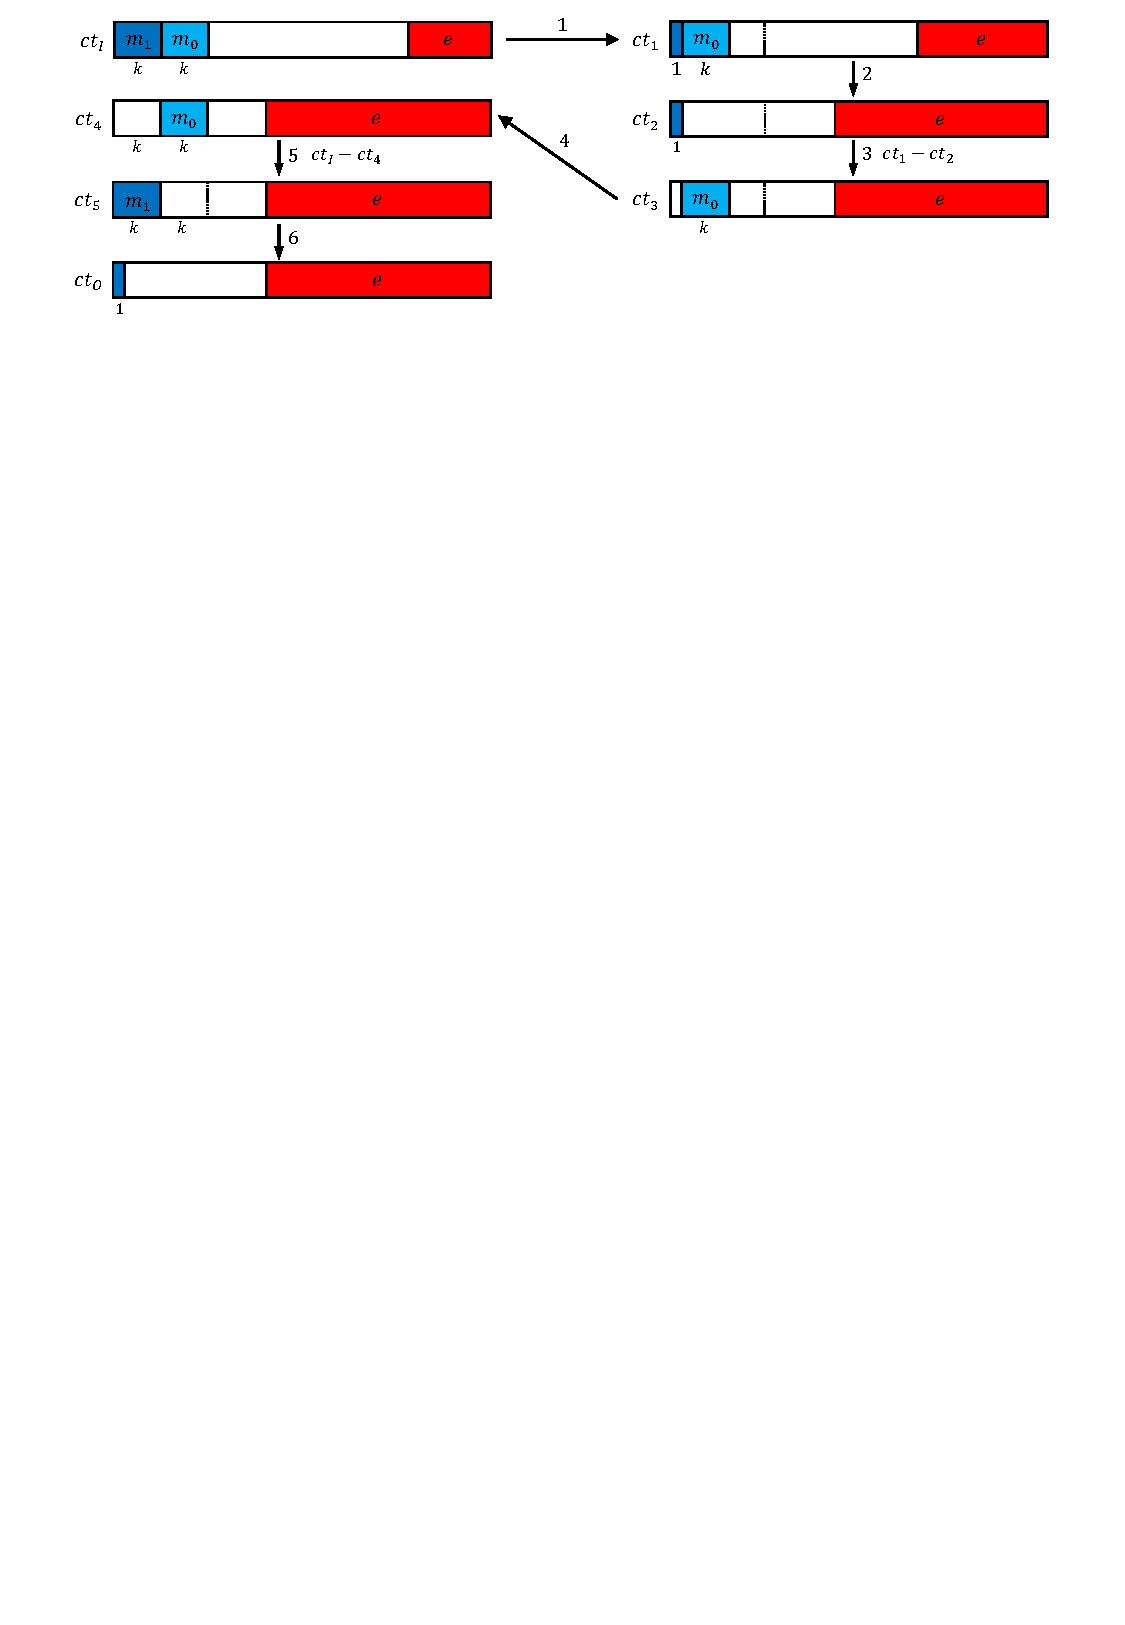
\includegraphics[width=0.75\linewidth]{figure/comparison.pdf}
%    \end{center}
%     \vspace{-0.5em}
%       \caption{A plaintext illustration in \cref{algo: 2kHMSB}. 
%       Each rectangle represents a decrypted plaintext while the left is 
%       the most significant bit.
%       The blue-colored region is the bits occupied by the message, 
%       the red-colored field is the bits filled with noise, 
%       and the white part is the bits set to zero.} 
%    \label{fig: comparison}
%    \vspace{-0.5em}
% \end{figure*}



%\subsubsection{Generality algorithm}
%\subsubsection{High-Precision Recursive HMSB}


% {\bf{Arbitrary Precision HMSB}}: 
% Given an input ciphertext $ct_{I} = {\rm LWE}_{n,q}(m)$, 
% where $m=\sum_{i = 0}^{t}2^{ik} \cdot m_{i}$.
% As shown in \cref{algo: tkHMSB}, in generality, we shift the ciphertext
% $(tk-1)$bits to move the most $(tk-1)$bits of $m$ 
% and reserve the least $(k+1)$bits. 
% The goal of the next four steps (line 2-5) is to move $m_{0}$ from $m$ 
% in an encrypted form, which is the same as \cref{algo: 2kHMSB}. 
% After that, we get the ciphertext $ct_{5}={\rm LWE}_{n,q}(m-m_0)$ and the 
% $m-m_{0}$ can be regarded as a $tk$-bit precision plaintext.
% By adopting ${\rm HMSB}_{tk}$ to $ct_{5}$, we obtain $ct_{O}$
% that encrypts the MSB of $m$.

\begin{algorithm}[t!]
    % \tiny
    \caption{$\homcomp$}
    \label{algo: homcom}
    \SetKwInOut{Input}{Input}\SetKwInOut{Output}{Output}\SetKwInOut{Return}{Return}\SetKwComment{Comment}{$\triangleright$\ }{}
    \Input{Two ciphertexts $ct_{a} = \lwe(a), ct_{b} = \lwe(b)$.}
    \Input{Comparison operator $\cmp$.}
    \Input{A bootstrapping key $\bBK$.}
    \Output{A LWE ciphertext $ct_{O} = \lwe(c)$
    where $c = 1$ if $a$ $\cmp$ $b$ is True, else $c = 0$.}
    \Switch{$\cmp$}
    {
        \lCase{$\geq$}{$ct_O \leftarrow \homgate((\hmsb(c_a-c_b), \reg{NOT}))$} \\
        \lCase{$>$}{$ct_O \leftarrow \hmsb(c_b-c_a)$} \\
        \lCase{$\leq$}{$ct_O \leftarrow \homgate(\hmsb(c_b-c_a), \reg{NOT})$} \\
        \lCase{$<$}{$ct_O \leftarrow \hmsb(c_a-c_b)$} \\
        \uCase{$==$}
        {
            $ct_O \leftarrow \homgate(\hmsb(c_a - c_b),\hmsb(c_b - c_a), \reg{NOR})$ \\
        }
        \uCase{$\ne$}
        {
            $ct_O \leftarrow \homgate(\homcomp(ct_a, ct_b, ==), \reg{NOT})$ \\
        }
    }
    % \uIf{$\cmp$ is $\geq$}
    % {
    %     $ct_O \leftarrow \homgate((\hmsb(c_a-c_b), \reg{NOT}))$ \\
    % }
    % \uElseIf{$\cmp$ is $>$}
    % {
    %     $ct_O \leftarrow \hmsb(c_b-c_a)$ \\
    % }
    % \uElseIf{$\cmp$ is $\leq$}
    % {
    %     $ct_O \leftarrow \homgate(\hmsb(c_b-c_a), \reg{NOT})$ \\
    % }
    % \uElseIf{$\cmp$ is $<$}
    % {
    %     $ct_O \leftarrow \hmsb(c_a-c_b)$ \\
    % }
    % \uElseIf{$\cmp$ is $==$}
    % {
    %     $ct_O \leftarrow \homgate(\hmsb(c_a - c_b),
    %      \hmsb(c_b - c_a), \reg{NOR})$ \\
    % }
    % \uElse
    % {
    %     $ct_O \leftarrow \homgate(\hmsb(c_a - c_b),
    %      \hmsb(c_b - c_a), \reg{NAND})$ \\
    % }
    \Return{$ct_{O} = {\rm LWE}(c)$}
\end{algorithm}
%\subsubsection{Homomorphic Comparison in EDBMS}
\subsubsection{$\homcomp$ Based on $\hmsb$}
Based on the arbitrary-precision $\hmsb$ algorithm devised above, we can carry
out arbitrary-precision comparisons between the queried attributes and the DB items.
Let $ct_a$ and $ct_b$ be the two LWE ciphertexts
that encrypt $a$ and $b$, and
$\cmp$ be the type of comparison to be performed ($\geq, >, \leq, <, ==, \ne$).
$\homcomp(ct_a, ct_b, \cmp)$ 
outputs an LWE ciphertext encrypting $1$
if the predicate $a$ $\cmp$ $b$ is true 
and $0$ if $a$ $\cmp$ $b$ is false.
The $\homcomp$ algorithm
can be easily constructed using $\hmsb$
with some additional homomorphic gates.
We summarize the exact arithmetic procedure for
$\homcomp$ in \cref{algo: homcom}. The complexity of our
$\homcomp$ algorithm can be expressed by the following lemma,
where the formal proof is given in the Appendix.

\begin{lemma}
    Given the two $tk$-bit ciphertext $ct_a$, $ct_b$ with
    a comparison operator $\homcomp$, the \cref{algo: homcom}
    outputs LWE ciphertext $ct_{O} = \lwe(c)$
    where $c = 1$ if $a$ $\cmp$ $b$ is True, else $c = 0$.
    The number of $\pbs$ evaluated by \cref{algo: homcom} 
    is $2t-1$ or $2t$.
    \label{lemma: homcomp}
\end{lemma}



% \begin{table}[htbp] 
%     \centering
%     \caption{Constructing \texttt{HomCom} using \texttt{HMSB}}
%     \vspace{-0.5em}
%         \begin{tabular}{cc}
%             \toprule
%             Comparison Type & Homomorphic Operation \\%\texttt{HomCom} & Operation \\
%             \midrule
%             $\texttt{HomComp}(c_1, c_2, \geq)$ & 
%             $\texttt{NOT}(\texttt{HMSB}(c1-c2))$\\
%             $\texttt{HomComp}(c_1, c_2, >)$ & 
%             $\texttt{HMSB}(c2-c1)$ \\
%             $\texttt{HomComp}(c_1, c_2, \leq)$ & 
%             $\texttt{NOT}(\texttt{HMSB}(c2-c1))$\\
%             $\texttt{HomComp}(c_1, c_2, <)$ & 
%             $\texttt{HMSB}(c1-c2)$ \\
%             $\texttt{HomComp}(c_1, c_2, ==)$ & 
%             $\texttt{HomComp}(c_1, c_2, \geq)$  
%             \texttt{AND} $\texttt{HomCom}(c_1, c_2, \leq)$ \\
            
            
%             \bottomrule
%         \end{tabular}
%     \label{tab:homcom}
% \end{table}




\subsection{Homomorphic Logic Aggregation}\label{block: minmax}
Most existing homomorphically encrypted database techniques~\cite{aphadb, heda} 
only support arithmetic aggregation (e.g., $\dbsum$ or $\dbavg$).
To support logic aggregation 
such as $\dbmin$, $\dbmax$, $\dbtopk$ and SQL statement such as $\orderby$, 
%we first propose a new set of two-input homomorphic operators to carry out
%$\dbmin$ and $\dbmax$ between two ciphertexts. Next, we propose an aggregation
we propose new two-input logic operators
that can be used to construct arbitrary logic aggregation functions. 
Due to space limitation, we use $\hommin$ as an example in this section. 
Our methodology applies generally to other types of logic aggregations.
% homomorphic $\dbmin$ operator $\hommin$
% and construct logic aggregation 
% $\homminagg$.


\begin{algorithm}[t!]
    % \tiny
    \caption{$\hommin$}
    \label{algo: hommin}
    \SetKwInOut{Input}{Input}\SetKwInOut{Output}{Output}\SetKwInOut{Return}{Return}
    \Input{Two LWE ciphertexts $ct_a = \lwe(a), ct_b = \lwe(b)$.}
    \Input{A bootstrapping key $\bBK$.}
    \Output{A LWE ciphertext $ct_{O} = \lwe(\dbmin(a,b))$.}
    $ct \leftarrow \homcomp(ct_a, ct_b, \leq)$ \\
    $C \leftarrow \cb(ct,\bBK)$ \\
    $ct_O \leftarrow \cmux(C, ct_a, ct_b)$ \\
    
    \Return{$ct_{O} = \lwe(\dbmin(a,b))$}
\end{algorithm}

\begin{algorithm}[t!]
    % \tiny
    \caption{$\homminagg$}
    \label{algo: homminagg}
    \SetKwInOut{Input}{Input}\SetKwInOut{Output}{Output}\SetKwInOut{Return}{Return}
    \Input{An RLWE ciphertext of the aggregated column $ct = \rlwe(\Tilde{m})$ where
    $\Tilde{m}_i = m_i$ for $i \in \mathbb{Z}_{\dbtabrowsize}$.}
    \Input{Filtered result $cf=
    (cf_{0}, cf_{1}, ... ,cf_{\dbtabrowsize - 1})$, where
    $cf_i = \lwe(f_i)$, $f_i = 0$ or $1$.}
    \Input{The pre-defined constant $\lwenan$.}
    \Input{A bootstrapping key $\bBK$.}
    \Output{A LWE ciphertext $ct_{O} = \lwe(\dbmin(m_{t_0}, ...,m_{t_{f-1}}))$ where
    $f =  {\textstyle \sum_{i=0}^{\dbtabrowsize - 1}}f_i$
    and $f_{t_0}, f_{t_1}, ..., f_{t_{f-1}} = 1$.}
    $\mathbf{ct} \leftarrow \sei(ct) = (ct_0, ct_1, ...,ct_{\dbtabrowsize-1})$ \\
    \For{$i = 0$ \KwTo $\dbtabrowsize - 1$}
    {
        $C_i \leftarrow \cb(cf_i, \bBK)$ \\
        $ct_i \leftarrow \cmux(C,ct_i,\lwenan)$ \\
    }
    \For{$i = 0$ \KwTo $\log_{2}{\dbtabrowsize} - 1$}
    {
        \For{$j = 0$ \KwTo $2^{\log_{2}{\dbtabrowsize} - i - 1} - 1$}
        {
            $ct_{2^{i+1}\cdot j} \leftarrow 
            \hommin(ct_{2^{i+1} \cdot j}, ct_{2^{i+1} \cdot j + 2^{i}}, \bBK)$ \\
        }
    }
    \Return{$ct_{O} = ct_{}0$}
\end{algorithm}

\subsubsection{Homomorphic $\dbmin$ and $\dbmin$ aggregation}
While there exists prior works~\cite{ckkscomparison, pegasus} 
for computing $\hommin$ and $\hommax$ operators, 
such techniques cannot be directly applied to a homomorphically encrypted database
due to two major obstacles.
The first obstacle is the low evaluation speed and unstable aggregation precision.
For example, while~\cite{ckkscomparison} can achieve high-precision $\hommin$ evaluation,
the method incurs a large number of latency overheads. On the other hand,
although~\cite{pegasus} can evaluate $\hommin$ and $\hommax$ relatively fast 
(but still slower than our proposed technique),
the technique suffers from the low precision ($<$ 6-bit) problem.
The second obstacle is how to evaluate logic aggregations
only on filtered rows. For a set of homomorphically filtered
results, the server cannot distinguish between an attribute value originally encrypted
to be zero and a filtered attribute that is set to be zero. Therefore, when performing
operations such as $\hommin$, we can produce incorrect results if we aggregate on invalid rows
that are marked as zeroes because they are filtered by the SQL statements.
% In a homomorphically encrypted database, 
% the number of selected records  
% and the values of selected records 
% are protected throughout the whole process.
% For instance, we could not distinguish the ciphertext of selected entries 
% between all entry ciphertexts
% $(ct_1, ct_2, ...,ct_{\abs{\mathcal{T}}_r})$.
% Therefore, it is hard to perform logic operators only on 
% the ciphertexts of selected entries.

To tackle the above two obstacles, we propose a new homomorphic logic aggregation procedure.
To overcome the first barrier, we introduce a new mechanism
to homomorphically evaluate $\dbmin$ (and $\dbmax$). We point out
that, for two numbers $a$ and $b$, prior works~\cite{ckkscomparison, pegasus} adopts the following formula
to compute the $\dbmin$ function.
\begin{equation}
    \dbmin(a, b) = (a \leq b)\text{ } ? \text{ }a\text{ } :\text{ } b
        % \begin{cases}
        %         a, a < b \\
        %         b, a \geq b
        % \end{cases}
    =
    \frac{a+b}{2} - \frac{\abs{a-b}}{2} 
    % \quad \reg{and} \quad
    % \texttt{MAX}(a, b) = \frac{a+b}{2} + \frac{\abs{a-b}}{2}
    \label{formula: sminmax}
\end{equation} 
However, evaluating the absolute function in HE will either be too slow
or too inaccurate. To avoid the absolute function, we propose to implement $\dbmin$ 
using the homomorphic comparison $\homcomp$ proposed in \cref{block: comparison}
and the homomorphic selector $\cmux$  defined in \cref{pre:he_circuits}. Essentially,
we compute
\begin{align}\label{eq:mincmux}
\hommin(a, b) = \gsw(a \leq b)\text{ }?\text{ }ct_a\text{ }:\text{ }ct_b,
\end{align}
where $\gsw(a\leq b)=\cb(\homcomp(ct_a, ct_b, \leq)$. Observe that Eq.~\eqref{eq:mincmux} is precisely Eq.~\eqref{eq:cmux},
and we sketch the full algorithm in \cref{algo: hommin}. That is, using $\homcomp$, 
$a\leq b$ can be homomorphically evaluated with high precision and high evaluation speed.
In addition, since $\cmux$ is also a fast operator (around $1000\times$ faster than
$\homcomp$), our $\hommin$ operator can be both faster and more accurate
than existing solutions~\cite{pegasus,ckkscomparison}.

% We exploit a simple fact that the conditional expressions
% of the initial $\dbmin$ definition could be converted 
% to the MSB value, which could be considered to control signal
% in a homomorphic selector.

% \begin{equation}
%     \begin{aligned}
%         \dbmin(a,b) = 
%             \begin{cases}
%                 a, a < b \\
%                 b, a \geq b
%             \end{cases}
%          = 
%             \begin{cases}
%                 a, \msb(a-b)=1 \\
%                 b, \msb(a-b)=0
%             \end{cases}
%         % \\
%         % \texttt{MAX}(a,b) = 
%         %     \begin{cases}
%         %         a, a \geq b \\
%         %         b, a < b
%         %     \end{cases}
%         % = 
%         %     \begin{cases}
%         %         a, MSB(a-b)=0 \\
%         %         b, MSB(a-b)=1
%         %     \end{cases}
%     \end{aligned}
%     \label{formula: minmax}
% \end{equation}

% \begin{equation}
%     \begin{aligned}
%         \hommin(ct_a, ct_b) = \texttt{CMUX}(CMSB, ct_a, ct_b) 
%         \\
%         \texttt{HomMAX}(ct_a, ct_b) = \texttt{CMUX}(CMSB, ct_b, ct_a)
%     \end{aligned}
%     \label{formula: homminmax}
% \end{equation}

% Here $CMSB$ is the RGSW ciphertext of $\texttt{MSB}(a-b)$.

Next, we solve the second obstacle by defining a constant ciphertext $\lwenan$
encrypting NaN, i.e., a `not a number' ciphertext. As detailed in
\cref{algo: homminagg}, the key idea is simple:
before comparing two LWE ciphertexts, 
we first use the encrypted filtered result $\gsw(\frakt)$
to pre-filter the input ciphertext $ct_i$ by computing 
\begin{align}\label{eq:lwenan}
\gsw(\frakt)\text{ }?\text{ }ct_i\text{ }:\text{ }\lwenan,
\end{align}
which is again a $\cmux$ operation. Note that,
in practice, $\lwenan$ can be initialized to be the largest 
value in the range of the plaintext message space (and the smallest
value in the case of $\hommaxagg$).
% before the $\dbmin$ computation.
% Thus the unsatisfactory rows will be replaced by the 
% gigantic ciphertexts and do not 
% affect the aggregation on satisfying rows.
Then, we can proceed to build a conventional 
min-tree of depth $\log_{2}{\dbtabrowsize}$
to calculate the minimum value over all rows in the attribute
column. 
The complexity analysis of the algorithm is provided in 
\cref{lemma: homminagg} (the proof can be found in the Appendix).

\begin{lemma}
    In \cref{algo: homminagg}
    the number of homomorphic \cmux gates is 
    $2\dbtabrowsize - 1$. 
    The number of homomorphic 
    $\cb$ operators is 
    $2\dbtabrowsize -1$,
    and the number of homomorphic 
    $\homcomp$ operators is
    $\dbtabrowsize -1$.
    \label{lemma: homminagg}
\end{lemma}

% \begin{figure}[t!]
%    \begin{center}
%    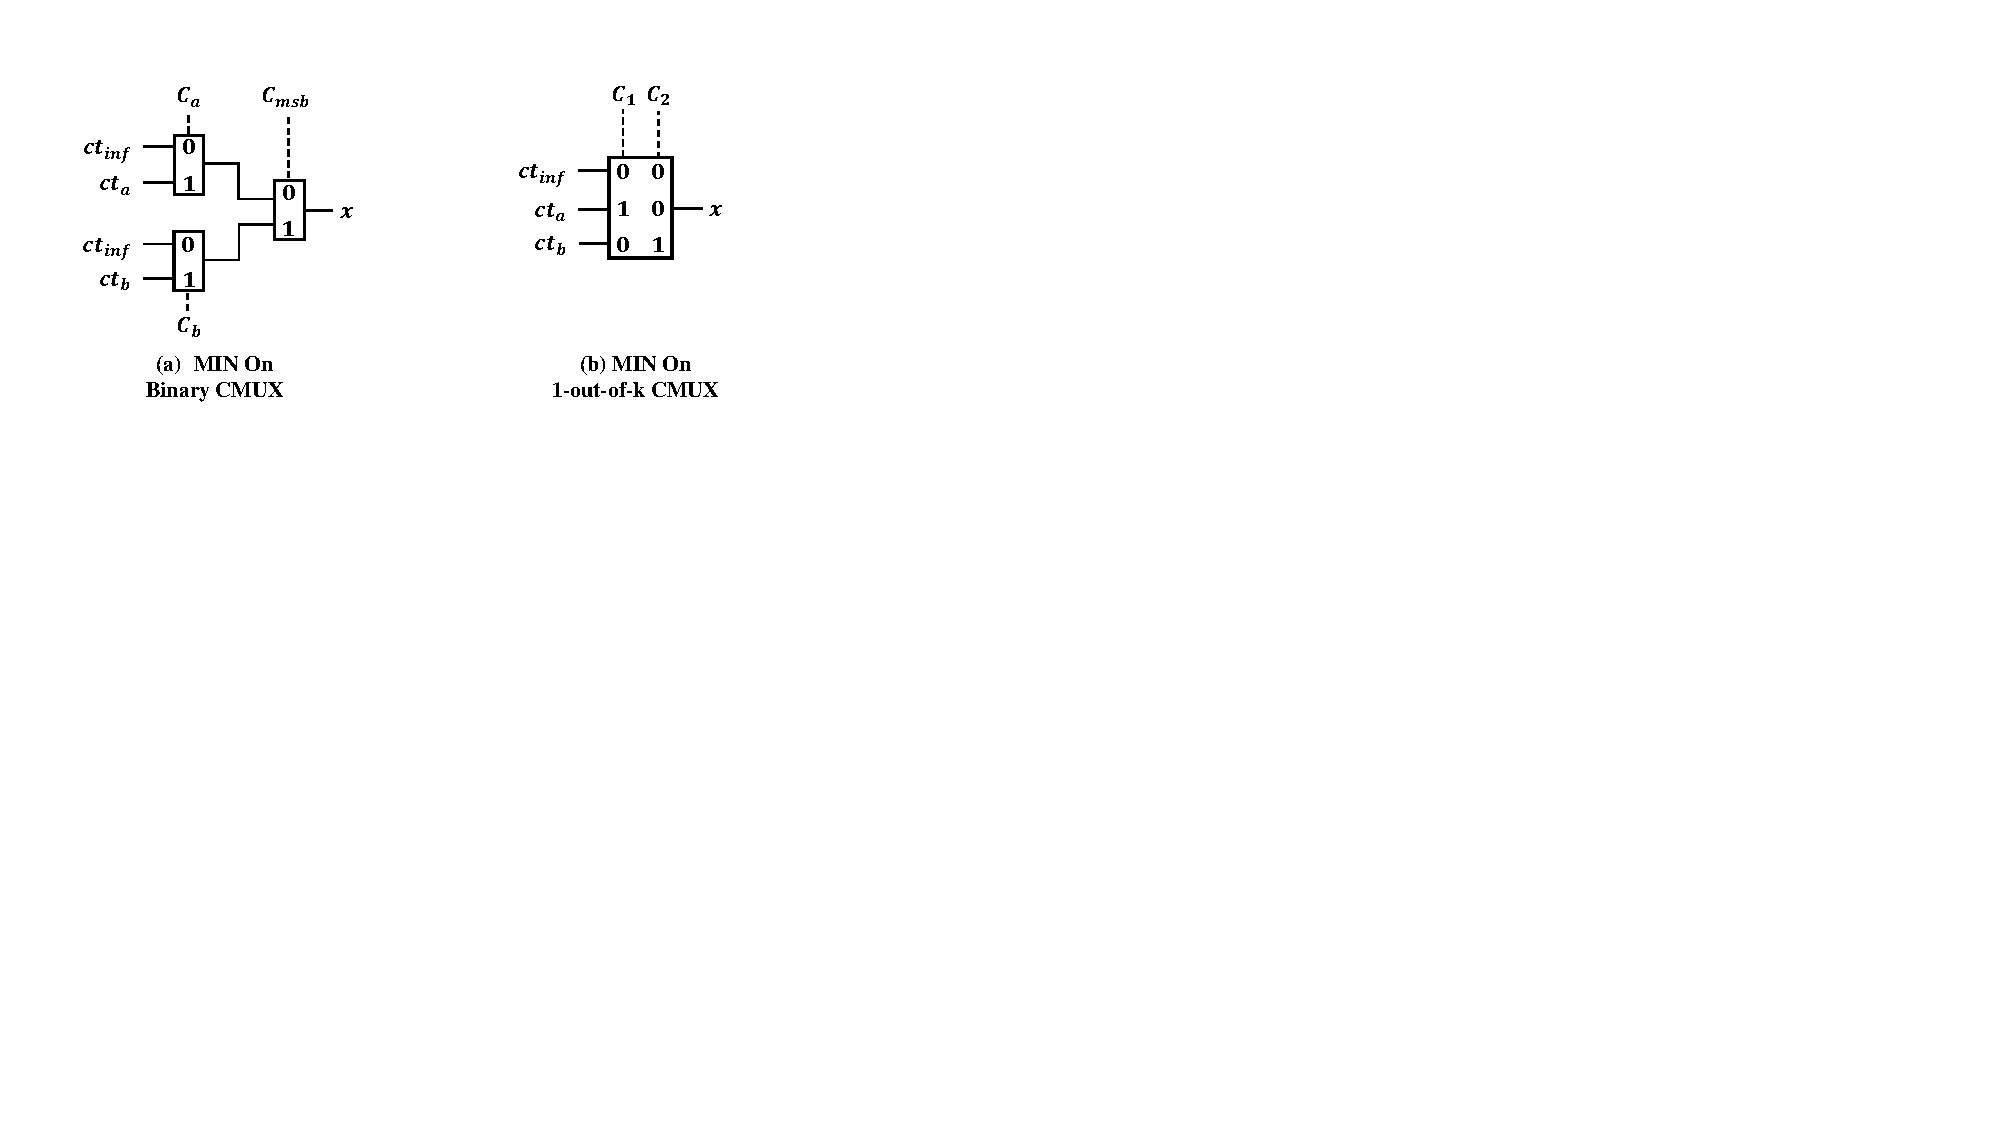
\includegraphics[width=\linewidth]{figure/mincmux.pdf}
%    \end{center}
%     \vspace{-0.5em}
%       \caption{A illustration of $\dbmin$ function on binary $\cmux$ and $\kcmux$.} 
%    \label{fig: mincmux}
%    \vspace{-0.5em}
% \end{figure}

% \begin{algorithm}[t!]
%     % \footnotesize
%     \caption{\texttt{1-out-of-k-CMUX}}
%     \label{algo: kcmux}
%     \SetKwInOut{Input}{Input}\SetKwInOut{Output}{Output}\SetKwInOut{Return}{Return}
%     \Input{$k$ $(\ge 2)$ LWE ciphertexts
%     $ct_0, ct_1, ...,ct_{k-1}$.}
%     \Input{$k-1$ control signals $C_1, C_2, ..., C_{k-1}$ where $C_t = 
%     \rgsw(1)$ and else are $\rgsw(0)$}
%     \Output{An LWE ciphertext $ct_{O} = ct_t$}
%     Initialize $ACC \leftarrow ct_0$. \\
%     \For{$i = 1$ \KwTo $k - 1$}
%     {
%         $temp_i \leftarrow ct_i - ct_0$ \\
%         $ACC \leftarrow ACC + temp_i \odot C_i$
%     }
%     \Return{$ACC$}
% \end{algorithm}

% \subsubsection{Optimizing of $\homminagg$}
% As shown in \cref{fig: mincmux} (a), we depict the \cref{algo: homminagg}
% in the case of two ciphertexts.
% Here, the $C_a$ and $C_b$ are 
% RGSW ciphertexts of the filtered result.
% They first control if $ct_a$ and $ct_b$ will be selected 
% in the latter $\hommin$ function. 
% The result $x_a$ is formulated as 
% \begin{equation}
%     x_a = \texttt{CMUX}(\texttt{CMUX}(ct_{max}, ct_a, C_a),
%     \texttt{CMUX}(ct_{max}, ct_b, C_b), C_{msb})
%     \label{formula: x_a}
% \end{equation}
% 
% However, as the homomorphic predicate evaluation result 
% is a set of LWE ciphertexts, we need to perform
% $\cb$ ciphertext conversion (also known
% as circuit bootstrapping~\cite{DBLP:journals/joc/ChillottiGGI20}) 
% in the first step (line 3-5).
% This takes most of the time in $\homminagg$ (nearly 90\%).
% To reduce the latency, we propose our optimized 
% $\kcmux$ in \cref{algo: kcmux}
% and merge the three $\cmux$
% with three control signals ($C_a, C_b,$ and $C_{msb}$)
% in \cref{fig: mincmux} (a) into one \texttt{1-out-of-3-CMUX}
% with control signals ($C_1$ and $C_2$) shown in \cref{fig: mincmux} (b).
% Here, the result $x_b$ is formulated as 
% \begin{equation}
%     x_b = \texttt{1-out-of-3-CMUX}(ct_{max}, ct_a, ct_b, C_1, C_2)
%     \label{formula: x_b}
% \end{equation}
% 
% The $C_1$ and $C_2$ are the 
% logical combination of $C_a, C_b,$ and $C_{msb}$.
% Therefore, we only need to perform two $\cb$ operators,
% which will reduce the latency
% by about $20\%$.
% Due to space constraints, we detail the exact optimization 
% of $\homminagg$
% in \cref{algo: ophomminagg} and provide
% complexity analysis with proof in \cref{lemma: ophomminagg}.

\subsubsection{Extending to Other Types of Aggregations}
As mentioned, the $\hommax$ and $\hommaxagg$ 
can be implemented in a very similar way as $\hommin$ and $\homminagg$,
except that $\lwenan$ needs to be defined as the smallest value
possible here.
% The \texttt{MIN/MAX-Index} could be constructed by
% changing the input $ct$ of the \cref{algo: homminagg} by the ciphertexts
% encrypts the index of records, \revise{we detail the exact algorithm in ...}.
Meanwhile, to achieve homomorphic $\orderby$, we propose a simple
swap function based on the $\hommin/\hommax$ operators as
% the key part of the sorting function is the swap between ciphertexts
% (including ascending swap and descending swap),
% which is
% We construct other
% operators like (\texttt{MIN/MAX-Index}, \texttt{Top-k}) and sorting
% based on our \texttt{HomMIN/MAX}
\begin{align}
    &\texttt{HASwap}(ct_a,ct_b) =  \hommax(ct_a, ct_b),
    \hommin(ct_a, ct_b)&
    \\
    &\texttt{HDSwap}(ct_a,ct_b) = \hommin(ct_a, ct_b),
    \hommax(ct_a, ct_b),&
\end{align}
depending the ascending ($\texttt{HASwap}$) and descending
($\texttt{HDSwap}$) orders requested by $\orderby$. 
Based on the homomorphic swap operators,
%Based on the homomorphic ascending/descending swap function,
it is easy to construct the sorting function by the existing sorting 
algorithms such as Bubble sort, quick sort~\cite{quicksort}, and 
bitonic sorting~\cite{bisort}.
%\revise{We detail the homomorphic ascending sorting algorithm in ...}. 
Finally, \texttt{Top-k} can be implemented by first executing a
descending $\orderby$, and then selecting the first $\textt{k}$ LWE 
ciphertexts.
\subsection{Homomorphic Arithmetic Aggregation}\label{block: LWEsPack}
To support homomorphic arithmetic aggregations 
(such as $\dbsum$, $\dbcount$, and $\dbavg$), 
the $\dbtabrowsize$ LWE ciphertexts which encrypt the filtered results
have to be packed in an RLWE ciphertext 
as arithmetic aggregation over LWE ciphertexts are slow.
In this section, we propose a new homomorphic ciphertext conversion
algorithm $\repack$ and the associated 
homomorphic arithmetic aggregations procedure.

\begin{algorithm}[t!]
    % \tiny
    \caption{$\repack$}
    \label{algo: lwespack}
    \SetKwInOut{Input}{Input}\SetKwInOut{Output}{Output}\SetKwInOut{Return}{Return}\SetKwComment{Comment}{$\triangleright$\ }{}
    \Input{$N$ LWE ciphertexts $(\lwe_0, \lwe_1, ...,\lwe_{N-1})$ where 
    $\lwe_i = \lwe^{n,q}_{\mathbf{s}}(m_i) = (b_i, \mathbf{a_i})$
    and $m_i = 0/1$. }
    \Input{A conversion key 
    $\reg{\mathbf{CK}}$.}
    \Input{A precision parameter $\delta$, range parameter $(u,v)$}
    \Output{An RLWE ciphertext $ct = \rlwe^{N,Q}_{\Tilde{s}}(\encode(\mathbf{m}))$,
    where $\mathbf{m}_{i} = m_i$ for $i \in \mathbb{Z}_{N}$}
     Let $\mathbf{b} \leftarrow [b_0, b_1, ...,b_{N-1}]$, 
     $\mathbf{A} \leftarrow [\mathbf{a_0}, \mathbf{a_1}, ..., \mathbf{a_{N-1}}]^{T} \in \mathbb{Z}_{q}^{N \times n}$\\
     % $ct_1 = \texttt{HomMVMul}(\mathbf{A},CK)$.
     $ct_1 \leftarrow \mathbf{CK} \diamond \mathbf{A}$
     \Comment*[r]{$ct_1 = \rlwe^{N,Q_1}_{\Tilde{s}}(\encode(\mathbf{A}\mathbf{s}))$}
     $ct_2 \leftarrow ct_1 + (\encode(\mathbf{b},0))$
     \Comment*[r]{$ct_2 = \rlwe^{N,Q_1}_{\Tilde{s}}(\encode(\mathbf{A}\mathbf{s} + \mathbf{b}))$} 
     $ct_3 \leftarrow\texttt{HomMod}(ct_2, q)$
     \Comment*[r]{$ct_3 = \rlwe^{N,Q_2}_{\Tilde{s}}(\encode(\mathbf{m+e}))$} 
     Generate the approximate polynomial $p(x)$ \\
     $ct \leftarrow \prnd(ct_3)$
     \Comment*[r]{$ct = \rlwe^{N,Q_3}_{\Tilde{s}}(\encode(\prnd(\mathbf{m})))$} 
    \Return{$ct = \rlwe^{N,Q}_{\Tilde{s}}(\encode(\prnd(\mathbf{m})))$}
\end{algorithm}

\subsubsection{Homomorphic ciphertext conversion $\repack$}
Existing works in converting LWE ciphertexts into
an RLWE ciphertext
include PEGASUS~\cite{pegasus} and 
the method of Chen \etal~\cite{conversionhaochen}.
% Both their methods can only achieve one competitive performance 
% in latency and precision.
% The key idea of 
% Pegasus~\cite{pegasus} in ciphertext conversion 
% consists of homomorphically evaluating LWE partial decryption as well as 
% homomorphically evaluating modulo $q$ on an RLWE ciphertext encrypting secret key.
% Both two operations can be achieved 
% by arithmetic homomorphic circuits~\cite{helib,ckksbootsparse,ckksbootvariance}.
Taking advantage of SIMD packing arithmetic homomorphic circuits, 
PEGASUS~\cite{pegasus}
performs fast ciphertext conversion but suffers from the low-precision 
problem due to the noise growth in homomorphic arithmetic circuits.
In contrast, Chen \etal~\cite{conversionhaochen} packs the
LWE ciphertexts by evaluating a series of
recursive homomorphic automorphisms~\cite{helib}.
We point out that Chen \etal~\cite{conversionhaochen}
enjoys high-precision packing capability, but 
induces a higher amount of latency overheads.
% This approach achieves high-precision packing but is 
% limited to a small size.
% When the packing size of LWE ciphertexts is large, 
% the latency is still very high.

%Unfortunately, in an encrypted database setting, 
Here, we design a homomorphic $\repack$ algorithm that
achieves both, a fast algorithm that can accurately
pack a set of LWE ciphertexts into one RLWE ciphertext.
%and high-precision format conversion.
% In \NAME, we propose our homomorphic ciphertext conversion method
% for homomorphically encrypted database
% which achieves low latency and high precision.
Our critical insight is that, in a homomorphically encrypted database, 
the predicate results are in a very limited range, e.g., usually only
0's and 1's to express the logical validity of the database entries.
Thus, we can actually ``correct'' the errors on the low-precision ciphertext to 
obtain a high-precision ciphertext. 
% To be more specific, we first
% execute the fast repack algorithm proposed in~\cite{pegasus} on
% a set of LWE ciphertexts to produce

% Then, we evaluate an additional $\Round$ function on the repacked RLWE
% ciphertext to homomorphically remove the noise $e$. 
% % the objective of our new conversion algorithm is to convert 
% %$ct = \rlwe(\encode(\mathbf{m}))\text{ where } $\bm \ni m_i = 0\pm e\text{ or }1\pm e$
% Concretely, we wish to convert
% $ct=\rlwe(\encode(\mathbf{m}))$ into $ct' =  \rlwe(\encode(\mathbf{m'}))$ such that 
% $m'_i = \Round(m_i)$, and that
% $m'_i$ contains less noises than $m_i$ for all $i\in|\bm|$.


The detailed algorithm $\repack$ involves the following steps.
First of all, in \cref{algo: lwespack},
we are given $N$ LWE filtering results $\lwe_0, \lwe_1, ...,\lwe_{N-1}$
where $\lwe_i = \reg{LWE}_{\mathbf{s}}^{n,q}(m_i) = (b_i, \mathbf{a_i})$
with a  conversion key 
$\reg{\mathbf{CK}}$.
On Line 1, we follow~\cite{pegasus} and rearrange the ciphertexts to 
construct a ciphertext matrix
$\mathbf{A} = [\mathbf{a_0}, \mathbf{a_1}, ..., \mathbf{a_{N-1}}]^{T} 
\in \mathbb{Z}_{q}^{N \times n}$ and a ciphertext vector 
$\mathbf{b} = [b_0, b_1, ...,b_{N-1}] \in \mathbb{Z}_{q}^{N}$.
Next, on Line 2, we evaluate the 
homomorphic matrix multiplication
$\mathbf{CK} \diamond \mathbf{A}$ 
to get $ct_1 = \rlwe^{N,Q_1}_{\Tilde{s}}(\encode(\mathbf{A}\mathbf{s}))$,
where $\encode$ stands for the CKKS encoding 
function~\cite{DBLP:conf/asiacrypt/CheonKKS17}.
Then, on Line 3, we homomorphically add $\bb$ to $ct_1$ and get $ct_2 = \rlwe^{N,Q_1}_{\Tilde{s}}(\encode(\mathbf{A}\mathbf{s} + \mathbf{b}))$.
After the above transforms, we obtain the ciphertext $ct_2$
encrypting $\mathbf{A}\mathbf{s}+\mathbf{b} = \mathbf{m} + t\mathbf{q}$.
To remove the $t\mathbf{q}$ term, on Line 4, 
we follow~\cite{ckksbootstrap,ckksbootsparse, ckksbootvariance, sinemod} 
to apply \texttt{HomMod} to the \texttt{mod} $q$ function 
homomorphically on $ct_2$, and get
$ct_3$. %i$ = \rlwe^{N,Q_2}_{\Tilde{s}}(\encode(\mathbf{m+e}))$.
At this stage, we obtain a packed but imprecise $\rlwe$ ciphertext 
$ct_3 = \rlwe(\encode(\mathbf{m}))$ encrypting
the vector of messages $\bm$ packed from the input. Here, we observe that for each $m_i\in\bm$,
$m_i$ equals either $1\pm e$ or $0\pm e$, where the noise $e$ 
in inevitably added via the above transforms.

To correct the errors, on Line 5 in \cref{algo: lwespack}, 
we generate a polynomial $\prnd(x)$ to approximate the rounding function $\Round(x)$.
% Similar to the bootstrapping function, to evaluate an approximate
% homomorphic rounding function over RLWE ciphertexts, we need
% to construct a polynomial that approximates the behavior
% of a rounding function.
%As it is not easy to  evaluate a round function
%via homomorphic arithmetic circuits directly, 
%we generate a high-degree polynomial to 
% approximate the target round function.
Following~\cite{ckksbootsparse}, given an interval $[u,v]$ and a pre-defined 
precision parameter $\delta$, we want to obtain
a polynomial $\prnd(x) =  {\textstyle \sum_{i=0}^{n-1}}a_ix^i $ such that
\begin{equation}
\forall x \in [u,v],  |\prnd(x)-\round{x} | < 2^{-\delta}, \label{formula: appro}
\end{equation}
where $2^{-\delta}$ is negligible.
%This question is a classical problem in approximation theory.
Based on the equioscillation theorem~\cite{equioscillation}, $\prnd(x)$
is the best possible approximation of the round function
if and only if 
\begin{align}
&\exists x_0 \leq ... x_i ... \leq x_n \in [u,v], &\\
&\prnd(x_i) - \round{x}= \epsilon(-1)^{i}|\prnd(x) - \round{x}|_{\infty} &
\label{formula: equioscillation}
\end{align}
where $\epsilon$ = $\pm 1$.
Taking \cref{formula: equioscillation} as the judgment condition, 
we can construct the Remez iteration algorithm~\cite{remez} to 
obtain the polynomial $p(x)$ meets the requirement of \cref{formula: appro}.
Upon obtaining $\prnd(x)$, we can actually perform
the approximate homomorphic rounding function on Line 6. As
explained in \cref{pre:he_circuits}, $\prnd(x)$ can be directly applied
to the RLWE $ct_3$ produced on Line 4, and we get the final output
$ct =  \rlwe(\encode(\prnd(\bm)))$. Here, the guarantee
is that the noises in $\prnd(\bm)$ will strictly be smaller than 
that in $\bm$.

% Concretely, we wish to convert
% $ct=\rlwe(\encode(\mathbf{m}))$ into $ct' =  \rlwe(\encode(\mathbf{m'}))$ such that 
% $m'_i = \Round(m_i)$, and that
% $m'_i$ contains less noises than $m_i$ for all $i\in|\bm|$.
% as claimed.
% After generating the approximated round function $p(x)$, we can
% evaluate $p(x)$ homomorphically over the RLWE ciphertext $ct_3$,
% as explained in \cref{pre:he_circuits}.
% As $p(x) =  {\textstyle \sum_{i=0}^{n-1}}a_ix^i $ is a type of 
% polynomial functions, it could be implemented efficiently 
% by homomorphic arithmetic circuits as we introduced in \cref{pre:he_circuits}.
% Moreover, expressing the approximated function $p(x)$ 
% in a Chebyshev basis~\cite{chebyshevbasis}
% could optimize the evaluation process with a less 
% number of ciphertext multiplication~\cite{
% improvedboot, betterboot, ckksbootsparse, inverseboot}.  

\subsubsection{Homomorphic arithmetic aggregation}
Using the filtered results packed in an RLWE ciphertext $cf$ based on
the proposed $\repack$ operator described above, we can finally
aggregate over the target attribute.  Let the RLWE ciphertext
encrypting items in the column be $ct_a$, we describe how
to implement three types of conventional arithmetic aggregation functions, 
namely, $\dbcount$, $\dbsum$ and $\dbavg$.
%encrypt the vector of filtered result and the encrypted column of 
%aggregated attribute $ct_a$.
Note that the first two functions can be implemented using simple inner
products between ciphertexts. Concretely,
$\dbcount$ function can be implemented by the inner product between $cf$ and
the vector $I = (1, 1, ...,1)$, while $\dbsum$
is also an inner product between $cf$ and $ct_a$.
The homomorphic inner product of two RLWE ciphertexts can
be implemented over ciphertexts in both the slot format~\cite{gazelle, pegasus} 
or in the coefficient format~\cite{cheetah, heda}.
Furthermore, the $\dbavg$ function can be evaluated by 
%$\dbavg() = \frac{\dbsum()}{\dbtabrowsize} \times 
% (\frac{\dbcount)}{\dbtabrowsize})^{-1}$, in which
$\dbavg() = \dbsum()\times 
\dbcount()^{-1}$, where the inverse function 
%the $\frac{1}{\dbtabrowsize}$ is public and 
%the inversion function $(\frac{\dbcount()}{\dbtabrowsize})^{-1}$ 
can be implemented based on ~\cite{ckkscomparison}.

% The homomorphic modular reduction function is a central part
% of CKKS bootstrapping~\cite{ckksbootstrap}, 
% %which is a cryptography puzzle of the FHE research community.
% and a number of recent works~\cite{ckksbootsparse, ckksbootvariance, sinemod}
% have investigated the accuracy-efficiency trade-off for different
% approximation polynomials.
% Note that the exact
% homomorphic matrix multiplication algorithms can be found in~\cite{gazelle, pegasus}.
% To add the vector $\mathbf{b}$, 
% we add the encoding result $\encode(\mathbf{b})$ of the vector 
% into the first term 
% of the ciphertext $ct_1$
% and gets $ct_2 = \rlwe^{N,Q_1}_{\Tilde{s}}(\encode(\mathbf{A}\mathbf{s} + \mathbf{b}))$.
% encode the vector $\mathbf{b}$ into
% a polynomial $\encode(\mathbf{b})$ and add it into the first term 
% of the ciphertext $ct_1$.
% Followed by a homomorphic addition with the vector $\mathbf{b}$, 
% we perform the LWE decryption formula $\mathbf{A}\mathbf{s}+\mathbf{b}$
% except for the modulo function.
% While there is a vast amount of prior work~\cite{helib, gazelle, haochenONN, pegasus}
% on HE for matrix-vector multiplication, 
% none take a generally efficient approach in all applications.
% Need to discuss

%\step{Line 4, Modulo $q$}:

%propose their own algorithm to solve it.
% and we adapt the approach from ~\cite{ckksbootsparse}
% as this is not the research part of this paper.
%\section {Data Analysis on \NAME}
\section {Analyzing Aggregated Results}\label{Analysis}

Since prior works only focus on the design of SQL evaluated over encrypted data,
the capability of further data processing on the queried result is mostly left 
unexplored. Here, we first discuss how to efficiently bridge the gap between 
the database query and online data analysis, and then show
a case study using private decision tree evaluation.
% sortinghat 
% Main point: existing data analysis methods may not achieve the best efficiency
% when dealing with database results

\subsection{Bridging DB Aggregation and Data Analysis}\label{Analysis: Bridge}
%Statistical Data Analysis}
\begin{figure}[t!]
   \begin{center}
   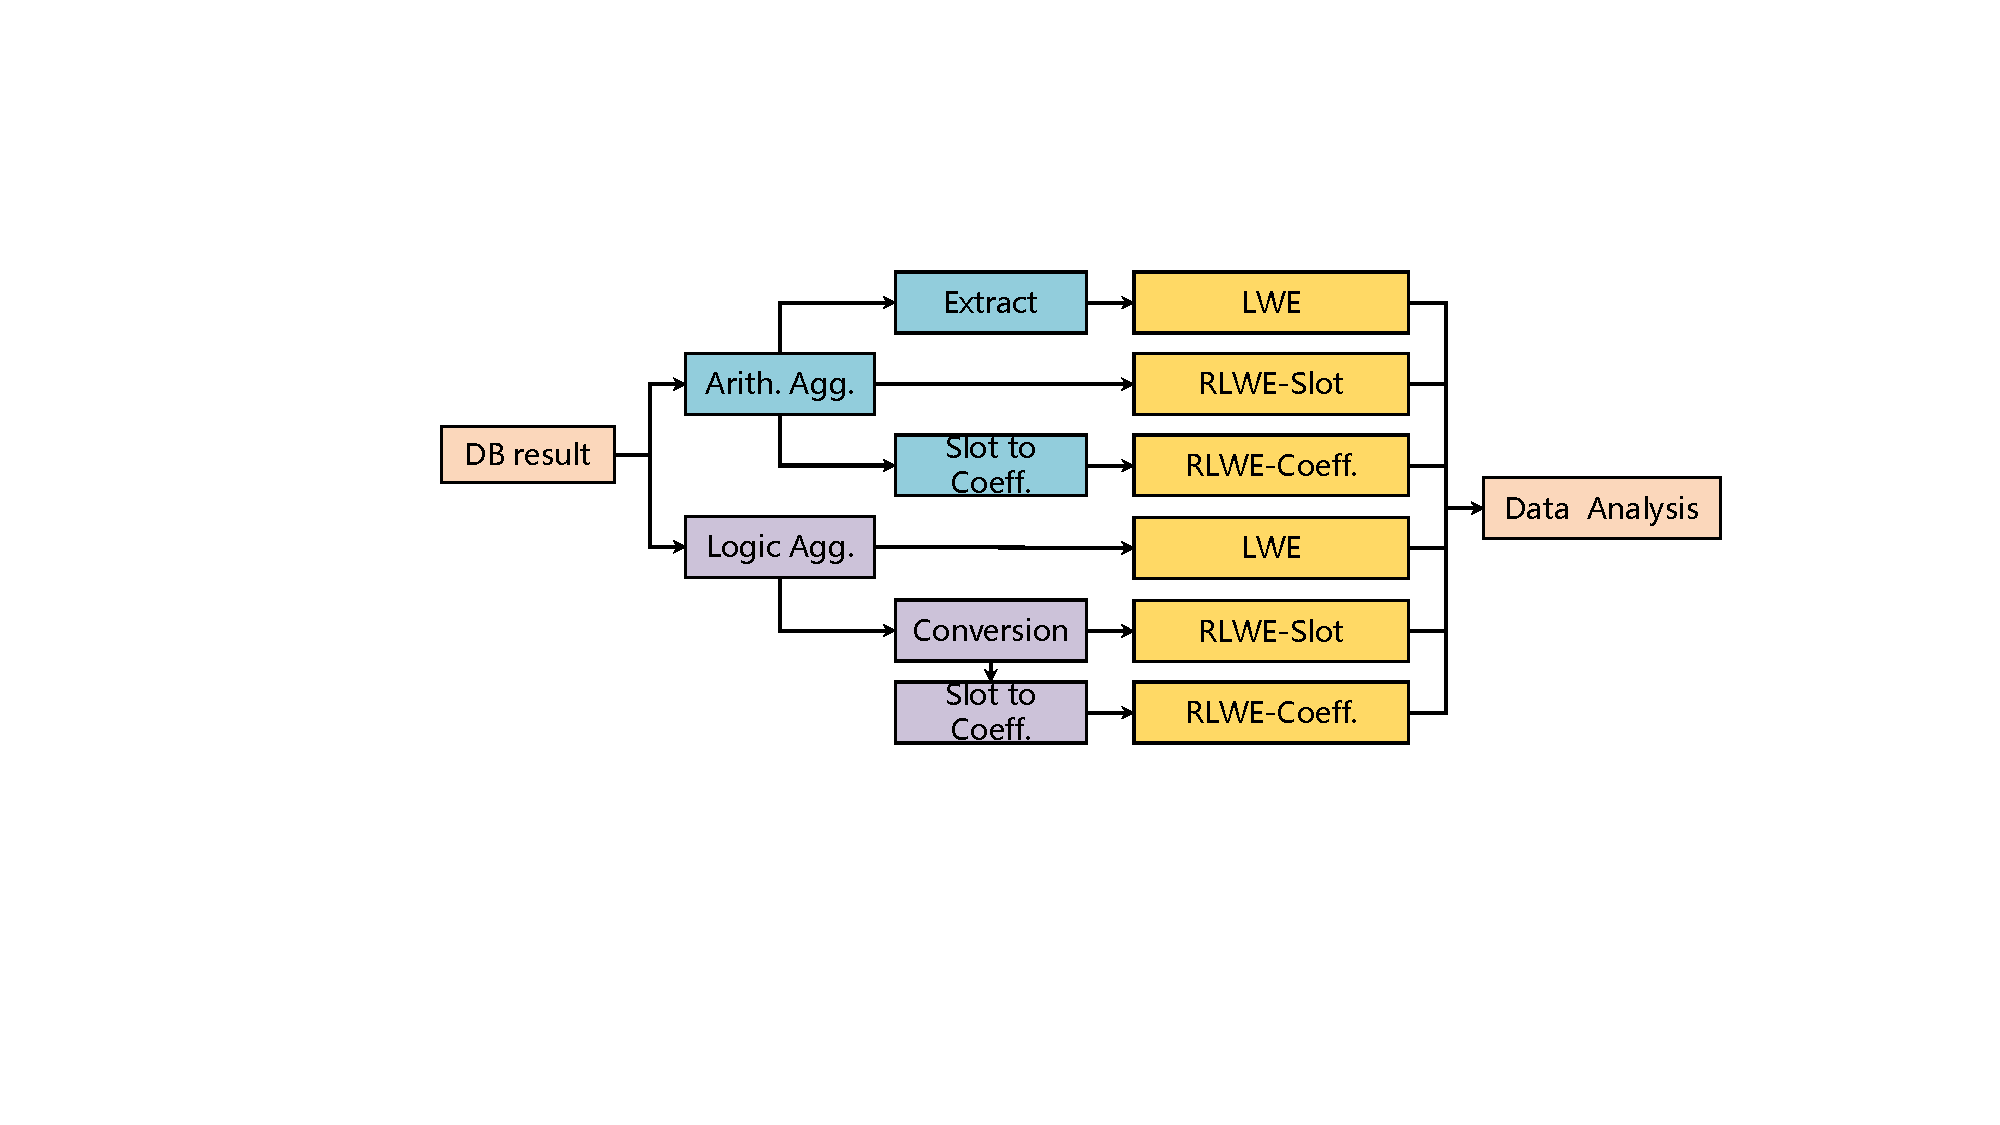
\includegraphics[width=\linewidth]{figure/conversion.pdf}
   \end{center}
    % \vspace{-0.5em}
      \caption{The conversion procedures to turn
      the aggregation results into data analysis inputs.} 
      \Description{Figure 4. Fully described in the text.}
   \label{fig: bridge}
   % \vspace{-0.5em}
\end{figure}

As shown in \cref{fig: bridge}, to support efficient data analysis algorithms
using both arithmetic and logic operators, we need to convert the queried
results into three different ciphertext formats: an LWE ciphertext ($\lwe$),
an RLWE ciphertext with slot encoding ($\rlweslot$), and an RLWE ciphertext
with coefficient encoding ($\rlwecoeff$).
% In order to evaluate general data analysis application which contains both
% arithmetic and logic circuits without client-server interactions,
% we summarize a bridging mechanism of 
% the arithmetic and logic aggregation result into 
% three different types of data analysis input in \cref{fig: bridge}.

% \textbf{Results from Logic Aggregation}: 
We first discuss the conversion algorithms for logic aggregations.
Note that, logic aggregation produces LWE ciphertexts as results. Therefore,
as sketched in \cref{fig: bridge}, there is no need of conversion if
the subsequent data analysis algorithm acts on LWE ciphertexts. For
other formats of ciphertexts, the following operators can be applied.
% and can be
% converted into other formats by the following operators.
% $\bullet$ \textbf{To LWE}: the logic aggregation results could be 
%     naturally applied to the data analysis application in the case of 
%     single value single data (SISD). 

$\bullet$ To $\rlweslot$: %\textbf{To $\rlweslot$}: 
Converting a set of LWE ciphertexts into an 
RLWE ciphertext in slot representation is precisely the proposed
$\repack$ operator described in \cref{block: LWEsPack}.

$\bullet$ To $\rlwecoeff$: %\textbf{To $\rlwecoeff$}: 
    Convert between the slot and coefficient forms for an RLWE ciphertext
    is well-studied in existing 
    literature~\cite{DBLP:journals/access/s2cc2s, betterboot, improvedboot, inverseboot}. 
    Thus, converting multiple $\lwe$ ciphertexts into an $\rlwecoeff$ ciphertext
    can be constructed by first applying the $\repack$ operator followed
    by the slot-to-coefficient transform.
%\end{itemize}

% \textbf{Results from Arithmetic Aggregation}: 
%\paragraph{Results from Arithmetic Aggregation}
Different from logic aggregations, the arithmetic aggregation results 
are RLWE ciphertexts in the 
slot representation. Hence, we can apply the following conversions to
the resulting ciphertext for subsequent data processing.
%\begin{itemize}

$\bullet$ To $\lwe$: %\textbf{To $\lwe$}: 
We can simply apply $\sei$ to
extract LWE ciphertexts from an RLWE ciphertext.
%     needs to first change the slot representation to the coefficient 
%     representation \texttt{CoeffToSlot}
%     and sample extracts the LWE ciphertexts.
% \textbf{To RLWE-Slot}: the arithmetic aggregation results could be 
%     naturally applied to the data analysis application in the case of 
%     single value multiple data (SIMD). 

$\bullet$ To $\rlwecoeff$: We can simply apply
the slot-to-coefficient transform above to convert 
$\rlweslot$ into $\rlwecoeff$~\cite{DBLP:journals/access/s2cc2s}.
% to fit some cases where coefficient 
% representation is more efficient in data analysis.
%\end{itemize}

% The arithmetic aggregation basically follows the 
% slot representation of RLWE ciphertext.


% As the LWE ciphertext 
% ciphertexts types, such as that between coefficient and slot
% representations~\cite{DBLP:journals/access/s2cc2s} 
% and that between SIMD and SISD 
% representations~\cite{DBLP:conf/sp/pegasus,DBLP:conf/acns/conversion}.
% There are three types of HE ciphertexts used in data analysis:
% LWE ciphertext, which is frequently used in SISD 

% \textbf{Logic Aggregation}: 

%{\bf{Private Decision Tree over Aggregated Results}}:
\subsection{Case Study: Private Decision Tree}\label{Analysis: PDTE}
Here, we take private decision tree evaluation (PDTE) as an example to combine the 
evaluation flows of \NAME.
A PDTE algorithm~\cite{sortinghat, pegasus} basically implements the following function 
over a set of LWE ciphertexts.
\begin{equation}
%(\lwe_{{\rm o}, 0}, \cdots, \lwe_{{\rm o}, \ell-1}) = \pdte(\lwe_{{\rm i}, 0}, \cdots, \lwe_{{\rm i}, d-1}, \algoweight),
\{\lwe_{{\rm output}, i}\}= \pdte(\{\lwe_{{\rm input}, j}\}, \algoweight),
\label{eq:pdte_conv}
\end{equation}
where a set of ciphertext inputs $\{\lwe_{{\rm input}, i}\}$ are
classified into $\ell$ output
ciphertext classes $\{\lwe_{{\rm output}, j}\}$ based on the pre-trained parameters $\algoweight$. 
Similar to existing works~\cite{sortinghat}, inputs and outputs of $\pdte$ are all LWE 
ciphertexts, since the evaluations of decision
trees consist mostly of non-linear operations. As mentioned,
we have two possible formats of ciphertext after the evaluation of an SQL query 
with aggregation: $\lwe$ and $\rlweslot$. Since logic aggregation naturally produces
an $\lwe$ ciphertext, the output can directly be fed into a PDTE algorithm. Meanwhile,
if we need to carry out PDTE over the arithmetically aggregated results, we can
simply apply $\sei$, as described in \cref{Analysis: Bridge}, and proceed with
the evaluation of \cref{eq:pdte_conv}. %Eq.~\eqref{eq:pdte_conv}. 

{\bf{Remark}}: Since most existing FHE-based PDTE algorithms are designed for 
two-party secure computing~\cite{pegasus, sortinghat}, the model parameters 
$\algoweight$ in \cref{eq:pdte_conv} are assumed to be known to the server. 
However, such an assumption does not always hold true in SDO, where the
data analysis algorithm can also be 
outsourced~\cite{shan2018practical,matsuoka2021virtual}. In particular,
switching PDTE to a computation outsourcing setting actually requires a complete
re-design of the evaluation protocol. Due to space limitation, we provide a complete 
description of our proposed SDO-orient PDTE algorithm based on the proposed
$\homcomp$ operator in the Appendix.

%A decision tree is a binary tree structure with a set of decision nodes and leaf nodes. It implements a mapping $\textbf{F}: \mathbb{Z}_{n}\rightarrow \{{w_0},...,{w_{\mathfrak{d}-1}}\}$, that maps an attribute vector $\mathbf{x} = ({x_0},...,{x_{n-1}})$ to a finite set of classification labels $\{{w_0},...,{w_{\mathfrak{d}-1}}\}$. The $i$-th decision node has threshold value ${t}_{i}$ and attribute index ${a}_{i}$ , while the $i$-th leaf node has label value ${w}_{i}$. Given a decision tree, the index of a node is its order as computed by breadth-first traversal, starting at the root with index 0. We denote $\mathfrak{d}$ as number of leaf nodes. If the tree is complete, the number of decision nodes is $\mathfrak{d} - 1$.

%The private decision tree is an encrypted version of the decision tree. After query processing, the server gets an aggregation result  $\mathcal{CR}$ = $(cr_0, cr_1,..., cr_{\lvert G \rvert})$ and client performs model encryption to obtain the private decision tree model $\mathcal{CM}$. During model encryption,  each threshold value $t_i$ is encrypted as $ct_i$, while each label value $w_i$ is encrypted as $cw_i$. Then the client sent the encrypted model $\mathcal{CM}$ to the server.

% Before Model Evaluation, the result of aggregation and the input of data analysis needs to be bridged through the function described in above. In the case of private decision tree, conventional technique \cite{sortinghat} \cite{pegasus} takes LWE ciphertexts as input, because the main operation in evaluating private decision tree is logic operation such as comparison. However, existing methods only useful under SQE model, and cannot be implemented in SDO model, because they require the decision tree parameters to be plaintext. Therefore, as an independent contribution, we propose a private decision tree evaluation algorithm \pdte, detailed in \cref{algo:pdte}, which can performs subsequent data analysis over both inputs and model parameters are encrypted.

%In \cref{eva:pdte}, we demonstrate that our \pdte function achieves 12x to 326x better evaluation time on different datasets and input size compared with existing work \cite{sortinghat}.


% As the output of logic aggregation and arithmetic aggregation
% may be distinct ciphertext formats.

% dimension lifting 
% The \texttt{LWEsPack} reaches good performance in the pack of 
% a lot of LWE ciphertexts.
% We aim to design an efficient 
% dimension-lifting \texttt{LWEToRLWE} algorithm
% that only performs one LWE ciphertext to an RLWE ciphertext. 
% Existing work ~\cite{conversionhaochen}

% Particularly, Chen~\cite{conversionhaochen} recently presented 
% a key-switching algorithm for LWE ciphertexts of 
% the same lattice dimension. 
% PEGASUS~\cite{pegasus} modify their algorithm for the dimension n > n. 
% We consider the case of dimension n < n 
% and propose a general dimension-switching algorithm.
\begin{table}[t!] 
    \centering
    \caption{The Proposed Parameter Sets}
    \vspace{0em}
        \begin{tabular}{cc}
            \toprule
            Ciphertext &  Parameters\\
            \midrule
            LWE & $n=672, \upint{\log_{2}{q} } = 32$\\
            RLWE & $N=65536, \upint{\log_{2}{Q} } = 653$\\
            RGSW & $N'=2048, \upint{\log_{2}{Q'} } = 64$\\
            % \multirow{3}*{LWE} & $n = 672, sd = 2^{-16}, 
            % \upint{\log_{2}{q} } = 32$ \\
            % & $n = 1024, sd = 2^{-25}, 
            % \upint{\log_{2}{q}} = 32$ \\
            % & $n = 2048, sd = 2^{-52}, 
            % \upint{\log_{2}{q}} = 64$ \\
            % \multirow{2}*{RWE} & $n = 1024, sd = 2^{-16}, 
            % \upint{\log_{2}{q} } = 32$ \\
            % & $n = 65536, \sigma = 3.19, 
            % \upint{\log_{2}{q_i} } = 32$ \\

            \bottomrule
        \end{tabular}
    \label{tab:parameters}
    % \vspace{-3mm}
\end{table}
\begin{table*}[t!] 
    \centering
    \caption{Qualitative Comparisons Between Homomorphic Comparison Algorithms}
    % \vspace{-0.5em}
        \begin{tabular}{cccccccc}
            \toprule
            & Kortekaas~\cite{aphadb}
            & Antonio \etal~\cite{revisiting}
            & Pegasus~\cite{pegasus} 
            & Liu \etal~\cite{largeprecision}
            & SortingHat~\cite{sortinghat} 
            & Cheon \etal~\cite{ckkscomparison} 
            & Ours\\
            \midrule
            Cipher-cipher comp.$^{+}$ & \yeah & \yeah & \yeah & \yeah & \nope & \yeah& \eyeah \\
            Full comparison & \yeah & \noyeah$^{++}$ & \yeah & \yeah & \yeah & \noyeah$^{++}$& \eyeah \\
            %16bit-precision & \yeah & \yeah & \nope & \yeah & \yeah & \yeah & \eyeah \\
            32-bit precision & \yeah & \yeah & \nope & \nope & \yeah & \nope & \eyeah \\
            %Predicate evaluation & \yeah & \nope & \yeah & \yeah & \yeah & \yeah & \eyeah \\
            Unbounded depth & \nope & \nope & \yeah & \yeah & \yeah & \nope & \eyeah\\
            Flexible parameter. & \noyeah$^{*}$ & \nope & \yeah & \nope & \nope & \noyeah$^{*}$ & \eyeah\\
            Efficiency & High & High & Low & Low & Low & High & High\\
            Storage & High & High & Low & Low & High & High & Low\\
            \bottomrule
        \end{tabular} \\
        {
        \footnotesize{
        %\begin{flushleft}
        $^{+}$Cipher-cipher comparison refers to the case where both of the 
        inputs to the comparison function are ciphertexts \\
        $^{*}$Changing encryption parameters requires the re-encryption the database 
        $^{++}$Do not support encrypted aggregations over results
        from equality comparison
        %\end{flushleft}
        }}
    \label{tab:homcom}
    % \vspace{-3mm}
\end{table*}
\section{Evaluation}\label{eva}
% In this section, we implement \NAME
% and thoroughly evaluate its efficiency. 
Throughout the experiments,
we wish to answer the following two main research questions (RQs).
\begin{itemize}
    \item {\bf{RQ1}}: How efficient are the individual components of \NAME
    compare to state-of-the-art (SOTA) methods? (\cref{sec:qual_comp}, \cref{eva: microbenchmarks}) 
    \item {\bf{RQ2}}: How does the performance of \NAME in specific SQL queries 
    and end-to-end data analysis benchmark compare to other methods? 
    (\cref{eva: sql_benchmark})
\end{itemize}
%We note in the first question, we want to benchmark

\subsection{Experiment Setup}\label{eva:Arch}
The entire \NAME is implemented using C++17 and 
compiled with GCC 10.3.0 based on Microsoft SEAL~\cite{codeseal},
%(an easy-to-use open-source homomorphic encryption library)
OpenPEGASUS~\cite{codepegasus}, and TFHEpp~\cite{codetfhepp}.
% , which are the state-of-the-art implementations
% of the CKKS and TFHE schemes.
For single-core microbenchmarks, the experiments are  carried out on 
an Intel Xeon Gold 6226R processor with 512GB of RAM. Meanwhile,
the experiments for the TPC-H benchmarks~\cite{tpc_h} reported in \cref{eva: sql_benchmark} are performed
on two servers with a total of four Intel Xeon Gold 5318Y processors with
96 cores and 1TB of RAM.
%\textbf{Instantiated Parameters}: 
The instantiated parameters are outlined in \cref{tab:parameters}, which provide 
at least 128-bit of security level according to~\cite{lweestimator}.
We fix the standard deviation 
$\sigma$ of the 
noise distribution $\chi$ and set the security level $\lambda$ 
to meet the Homomorphic Encryption Standard~\cite{HomomorphicEncryptionSecurityStandard}. 
It is noted that we actually achieved better security than the most relevant work HEDA,
as HEDA only guarantees an 80-bit security~\cite{heda}.

% Here, 
% we take $\sigma = 3.19 
% \approx 8/\sqrt{2\pi } $ and the resulting $\lambda = 128$-bit.




\subsection{Qualitative Assessments for $\homcomp$}\label{sec:qual_comp}
\begin{table}[t!] 
    \centering
    \caption{Benchmark Results for Homomorphic $\geq$}
    % \vspace{0em}
        \begin{tabular}{cccccc}
            \toprule
            Precision & Methods & \multicolumn{2}{c}{Latency (ms)} & \multicolumn{2}{c}{Ciphertext (kB)} \\
                 %&         & (ms)      &         & (kB) & \\
            \midrule
             \multirow{4}*{4} & PEGASUS~\cite{pegasus} & 681 & $37.83\times$ & 8 & $2\times$ \\
             & SortingHat~\cite{sortinghat} & 444 & $24.67\times$ & 10 & $2.5\times$ \\
             & Liu \etal ~\cite{largeprecision} & 2040 & $113\times$ & 16 & $4\times$ \\
             % & Antonio\cite{revisiting} & 70 & $3.89\times$ & 5 & $1.25\times$ \\
             & \textbf{Ours} & 18 & $1\times$ & 4 & $1\times$ \\
             \midrule
            % \midrule
            %  \multirow{4}*{8} & Pegasus~\cite{pegasus} & 3027& $56.06\times$ & 8 & $2\times$ \\
            %  & SortingHat~\cite{sortinghat} & 1030 & $19.07\times$ & 19 & $4.75\times$ \\
            %  & Liu~\cite{largeprecision} & 4439 & $82.2\times$ & 16 & $4\times$ \\
            %  % & Antonio\cite{revisiting} & 138 & $2.56\times$ & 10 & $2.5\times$ \\
            %  & \NAME & \textbf{54} & $1\times$ & \textbf{4} & $1\times$ \\
            % \midrule
             \multirow{4}*{16} & PEGASUS~\cite{pegasus} & --- & --- & --- & --- \\
             & SortingHat~\cite{sortinghat} & 2186 & $8.13\times$ & 38 & $2.38\times$ \\
             & Liu \etal~\cite{largeprecision} & 7992 & $29.71\times$ & 16 & $1\times$ \\
             % & Antonio\cite{revisiting} & 277 & $1.03\times$ & 20 & $1.25\times$ \\
             & \textbf{Ours}  & 269 & $1\times$ & 16 & $1\times$ \\
            \midrule
             \multirow{4}*{32} & PEGASUS~\cite{pegasus} & --- & --- & --- & --- \\
             & SortingHat~\cite{sortinghat} & 4329 & $7.67\times$ & 76 & $4.75\times$ \\
             & Liu \etal~\cite{largeprecision} & --- & --- & --- & ---\\
             % & Antonio\cite{revisiting} & 202 & $1.22\times$ & 40 & $2.5\times$ \\
             & \textbf{Ours}  & 564 & $1\times$ & 16 & $1\times$ \\
            \bottomrule
        \end{tabular}
    \label{tab:combenchmark}
    {\footnotesize{$-$ means
    the method does not support such bits of precision.}}
    % \vspace{-3mm}
\end{table}

\begin{figure*}[t!]
   \begin{center}
    \begin{subfigure}[b]{0.3\textwidth}
    \centering
    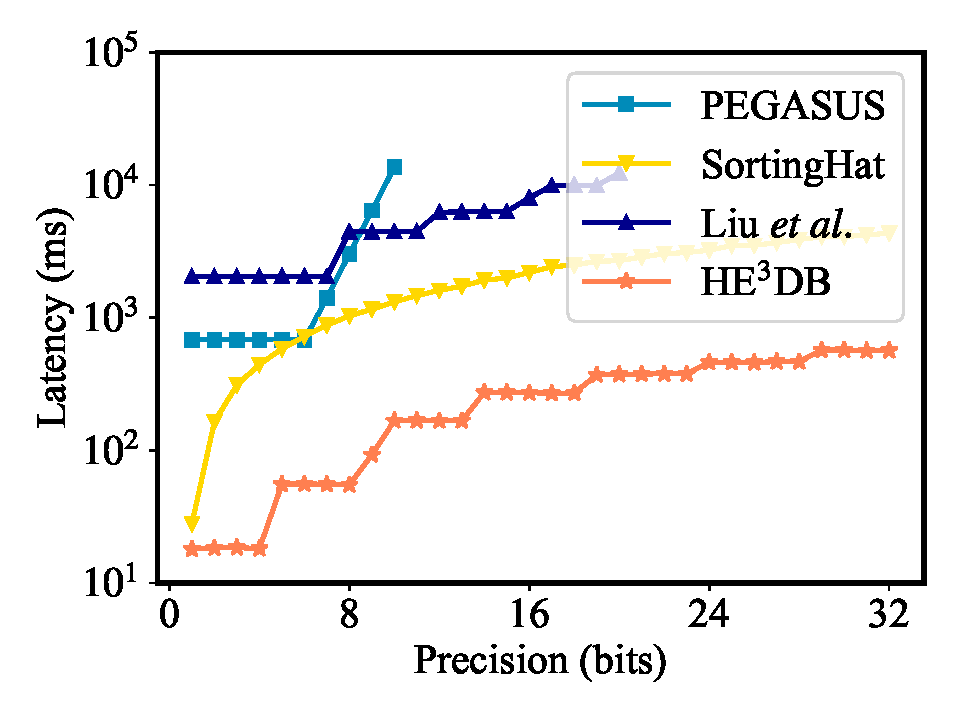
\includegraphics[width=\linewidth]{figure/com_micro_geq.pdf}
    % \vspace{-2em}
    \caption{Homomorphic $\geq$}
    \label{fig:homcompbench1}
    \end{subfigure}%
    \hfill
    \begin{subfigure}[b]{0.3\textwidth}
    \centering
    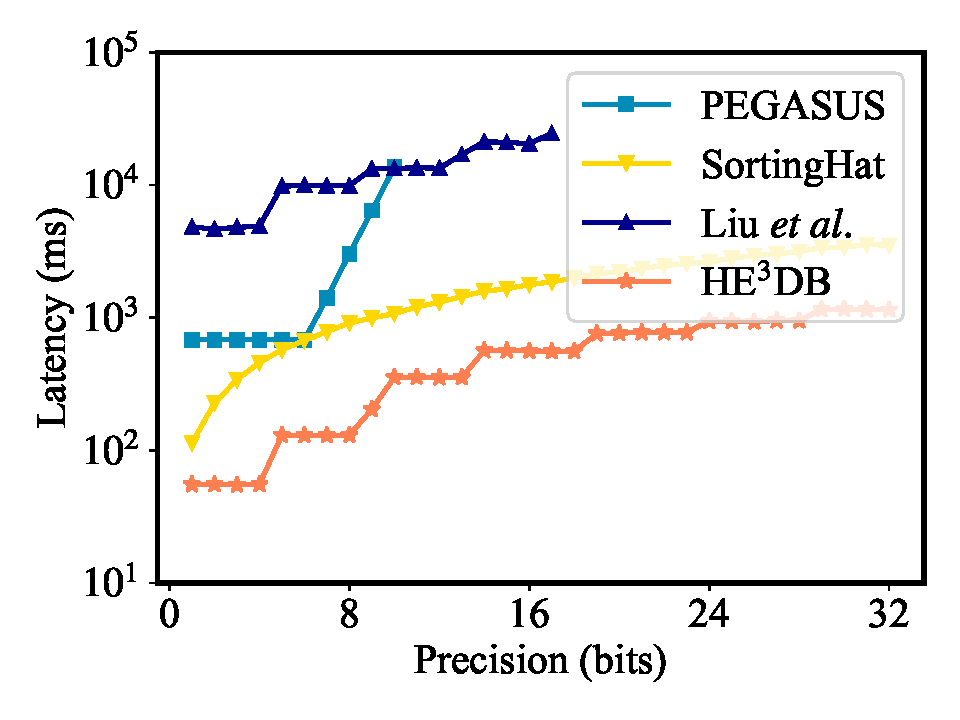
\includegraphics[width=\linewidth]{figure/com_micro_eq.pdf}
    % \vspace{-2em}
    \caption{Homomorphic $==$}
    \label{fig:homcompbench2}
    \end{subfigure}%
    \hfill
    \begin{subfigure}[b]{0.3\textwidth}
    \centering
    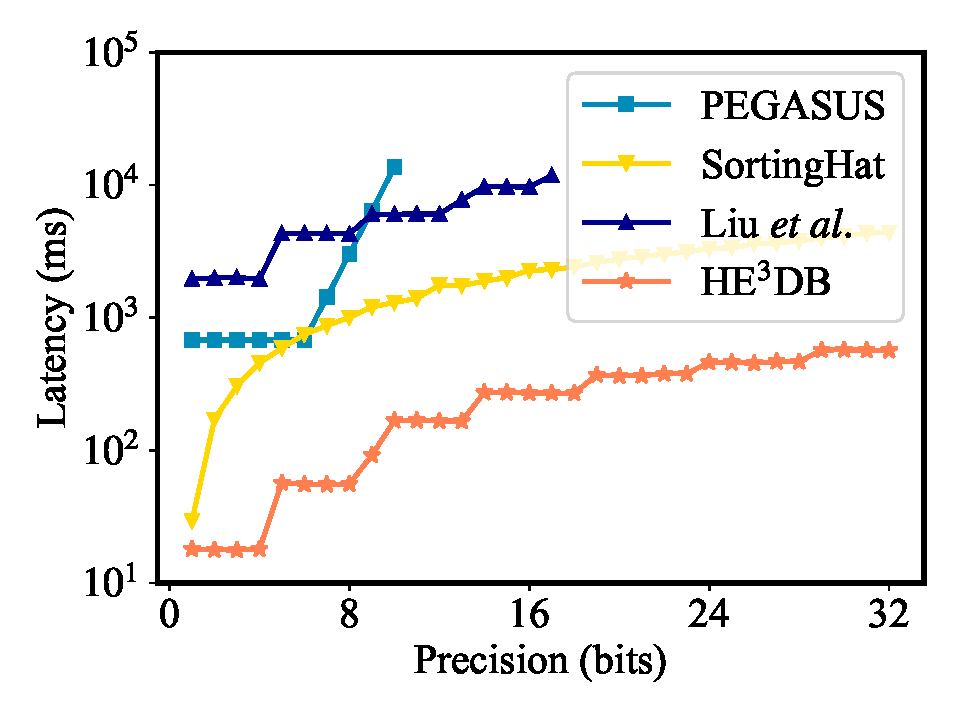
\includegraphics[width=\linewidth]{figure/com_micro_g.pdf}
    % \vspace{-2em}
    \caption{Homomorphic $>$}
    \label{fig:homcompbench3}
    \end{subfigure}%
   
   \end{center}
    % \vspace{-0.5em}
      \caption{Benchmark results for homomorphic comparison for the 
      $\geq, ==, >$ comparison operators 
       with varying bit precision.}
       \Description{Benchmark results for homomorphic comparison for the 
      $\geq, ==, >$ comparison operators 
       with varying bit precision. 
       The horizontal axis is the bits of precision, and the vertical axis is the latency. 
       Our results achieve competitive performance across different
       comparison operators}
   \label{fig: homcompbench}
   % \vspace{-0.5em}
\end{figure*}
Since $\homcomp$ is one of the key homomorphic operators proposed
in this work, we first compare our $\homcomp$ with other related 
homomorphic comparison algorithms qualitatively, and
defer quantitative results to \cref{eva: microbenchmarks}.
% have their own advantages and 
% method selection depends on the application.
In the beginning, we note that approaches like PEGASUS~\cite{pegasus} and the method 
proposed by Liu \etal~\cite{largeprecision} focus on evaluating
arbitrary logic
functions over homomorphically encrypted ciphertext,
%by proposing efficient or large-precision PBS algorithms
while \NAME concentrates on the design of a homomorphic comparison algorithm.
Therefore, our method achieves better comparison accuracy as well
as efficiency than~\cite{pegasus, largeprecision}. In contrast
to general methods, 
SortingHat~\cite{sortinghat} proposes an efficient plaintext-ciphertext 
comparison algorithm, where one of the inputs to the comparison
is known to the server. Nonetheless, under an SDO setting,
SortingHat shows poor efficiency for ciphertext-ciphertext
comparisons. The method of Antonio \etal~\cite{revisiting} 
encrypts the input in a bit-wise manner, where binary circuits
can be used to construct fast and high-precision
homomorphic comparison. However, due to the encoding scheme, 
the algorithm in~\cite{revisiting} produces
a comparison result of $\{-1,0,1\}$, which cannot be used as
filters for subsequent aggregations.
Similarly, the polynomial approximation technique proposed by 
Cheon \etal~\cite{ckkscomparison} cannot support encrypted 
aggregations over results from equality tests \texttt{==}, for the approximate polynomial evaluates
to $1/2$ when the inputs are equal.
On the other hand, some works also suggest to encrypt all database items bit-by-bit in a
SIMD manner to accelerate the comparison process~\cite{aphadb, khedr2015shield}.
%due to the noise growth of RLWE ciphertext 
%as we discussed in \cref{pre:he_type}.
However, in such approaches, the client encrypts the 
entire database using an {\it{a-priori}} fixed-set parameters 
that are dependent on
the pre-defined maximum predicate depth. As a result,
any query that requires more predicate evaluations than the
pre-defined maximum depth cannot be directly
evaluated. Here, the only solution is to re-encrypt
entire database using a new set of encryption parameters, which
can be too costly for SDO clients.
%respectively representing the \texttt{<}, \texttt{==} and \texttt{>}.
% However, Antonio's approach~\cite{revisiting} does not support 
% the encrypted database scenarios as the result of the comparison 
% could not perform logic gate operation between various predicates.

% Different from the above approaches, a line of works investigate
% how to utilize polynomial approximations 
% to evaluate homomorphic comparisons over RLWE 
% ciphertexts~\cite{ckkscomparison}. 
% By leveraging
% the SIMD capability of RLWE ciphertext,
% such algorithm can achieve fast evaluation speed when processing
% a large number of parallel comparisons.
% Nonetheless, both of their methods do not meet the elasticity requirement.


% However, changing encryption parameters in~\cite{aphadb} requires the re-encryption
% of the entire database, which can bring about severe communcation 
% burdens on the client side in practice.
% encrypted queries that are more complicated than such depth.
% We list the qualitative comparisons between existing methods and 
% provide quantitative comparisons in \cref{eva: microbenchmarks}.

% Since not all of the methods summarized
% in \cref{eva: microbenchmarks} have the same design objective,

\subsection{Evaluating Cryptographic Building Blocks}\label{eva: microbenchmarks}

\begin{figure*}[t!]
    \begin{minipage}[t]{0.5\linewidth}
    \centering
    \begin{subfigure}[b]{0.5\textwidth}
    \centering
    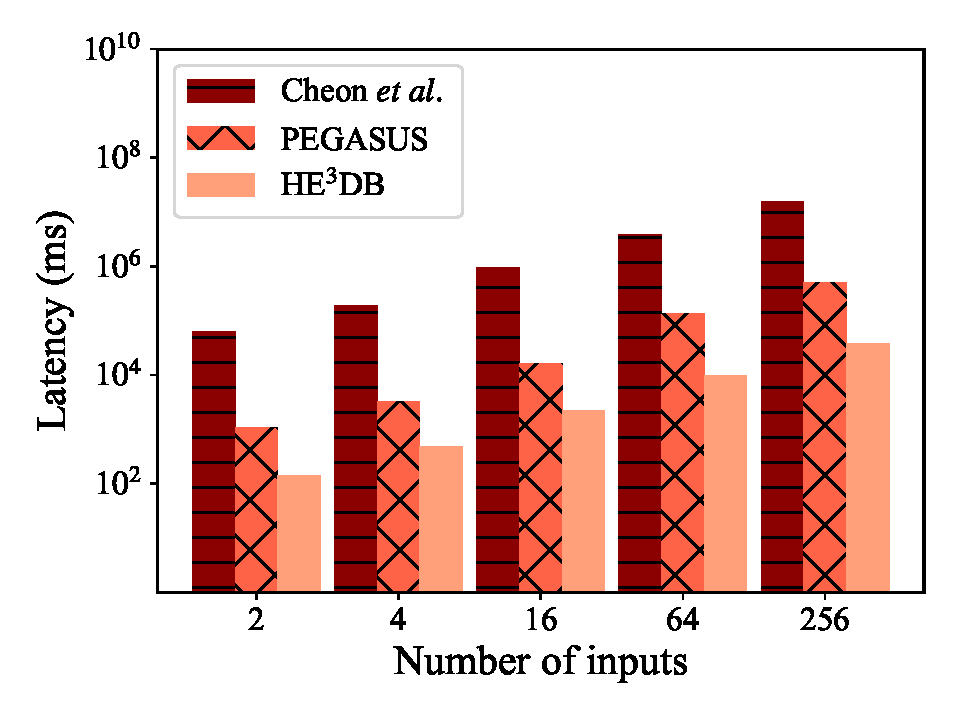
\includegraphics[width=\linewidth]{figure/minbench_4.pdf}
    % \vspace{-2em}
    \caption{4-bit $\dbmin$}
    \label{fig:homminbench4}
    \end{subfigure}%
    \hfill
    \begin{subfigure}[b]{0.5\textwidth}
    \centering
    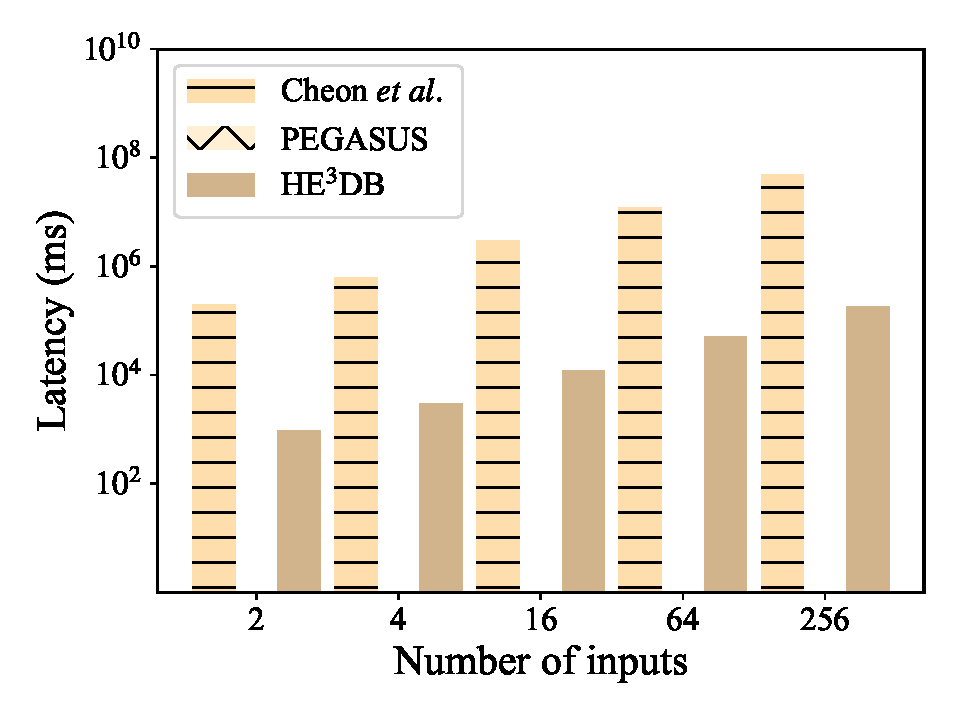
\includegraphics[width=\linewidth]{figure/minbench_16.pdf}
    % \vspace{-2em}
    \caption{16-bit $\dbmin$}
    \label{fig:homminbench16}
    \end{subfigure}%
    \caption{Benchmark results for Homomorphic $\dbmin$.}
    \Description{Benchmark results for Homomorphic $\dbmin$. The horizontal axis is the number of inputs, and the vertical axis is the latency. From the result, our performance is on average 
    around one order of magnitude faster than PEGASUS~\cite{pegasus}
    and two orders of magnitude faster than ~\cite{ckkscomparison}.}
    \label{fig: homminbench}
    \end{minipage}%
    \begin{minipage}[t]{0.5\linewidth}
    \centering
    \begin{subfigure}[b]{0.5\textwidth}
    \centering
    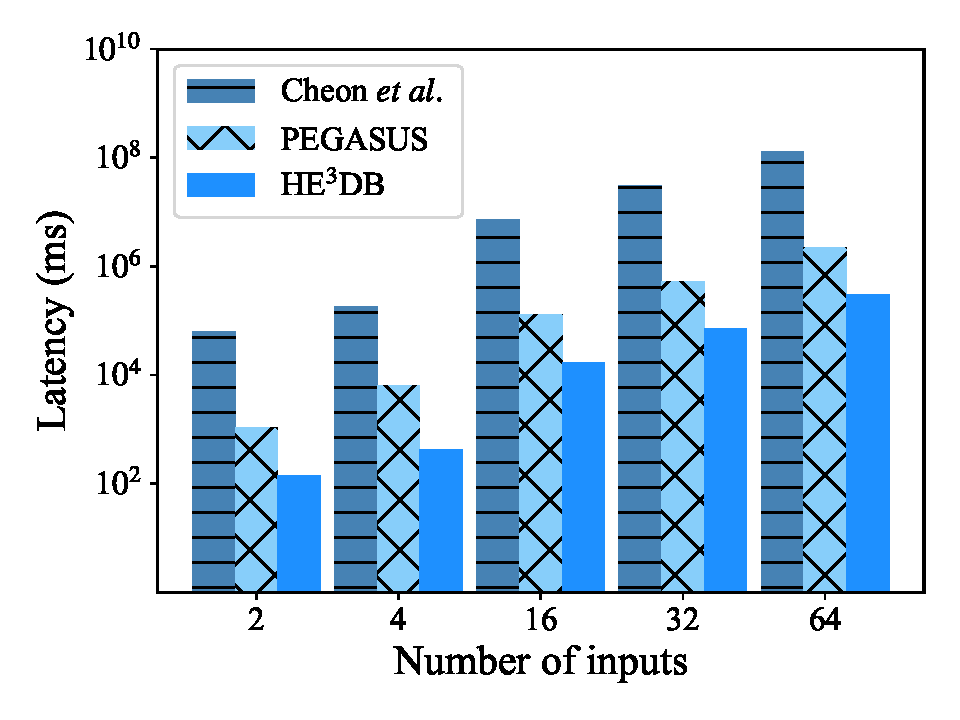
\includegraphics[width=\linewidth]{figure/sortbench_4.pdf}
    % \vspace{-2em}
    \caption{4-bit \orderby}
    \label{fig:homsortbench4}
    \end{subfigure}%
    \hfill
    \begin{subfigure}[b]{0.5\textwidth}
    \centering
    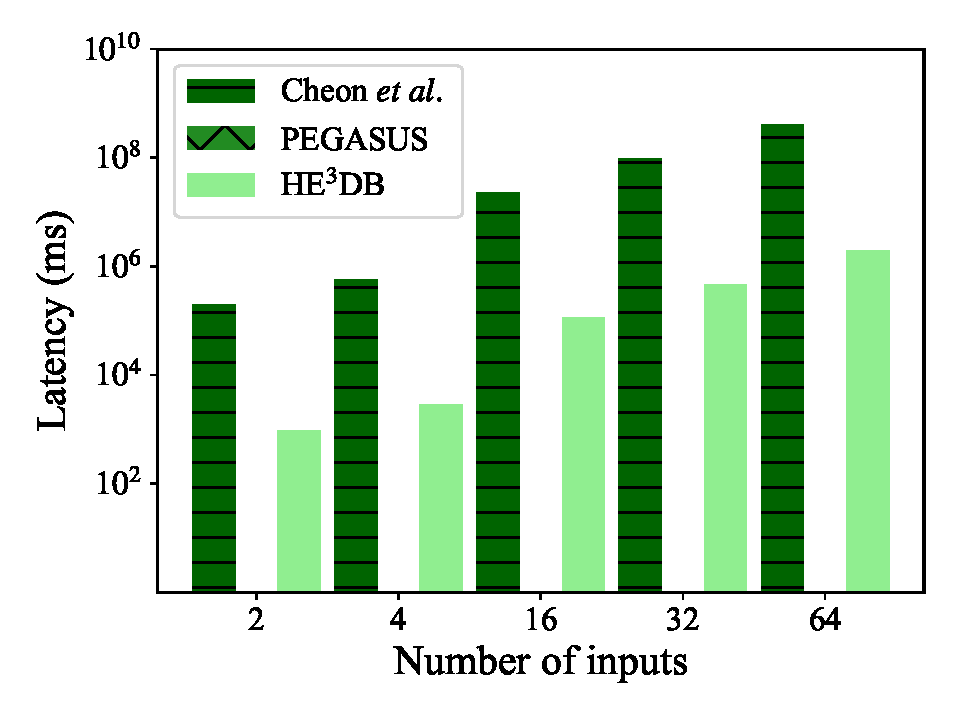
\includegraphics[width=\linewidth]{figure/sortbench_16.pdf}
    % \vspace{-2em}
    \caption{16-bit \orderby}
    \label{fig:homsortbench16}
    \end{subfigure}%
    \caption{Benchmark results for Homomorphic $\orderby$.}
    \Description{Benchmark results for Homomorphic $\orderby$. The horizontal axis is the number of inputs, and the vertical axis is the latency. From the results, our performance is on average 
    around one order of magnitude faster than PEGASUS~\cite{pegasus}
    and two orders of magnitude faster than ~\cite{ckkscomparison}.}
    \label{fig: homsortbench}
    \end{minipage}
   % \begin{center}
   %  \begin{subfigure}[b]{0.25\textwidth}
   %  \centering
   %  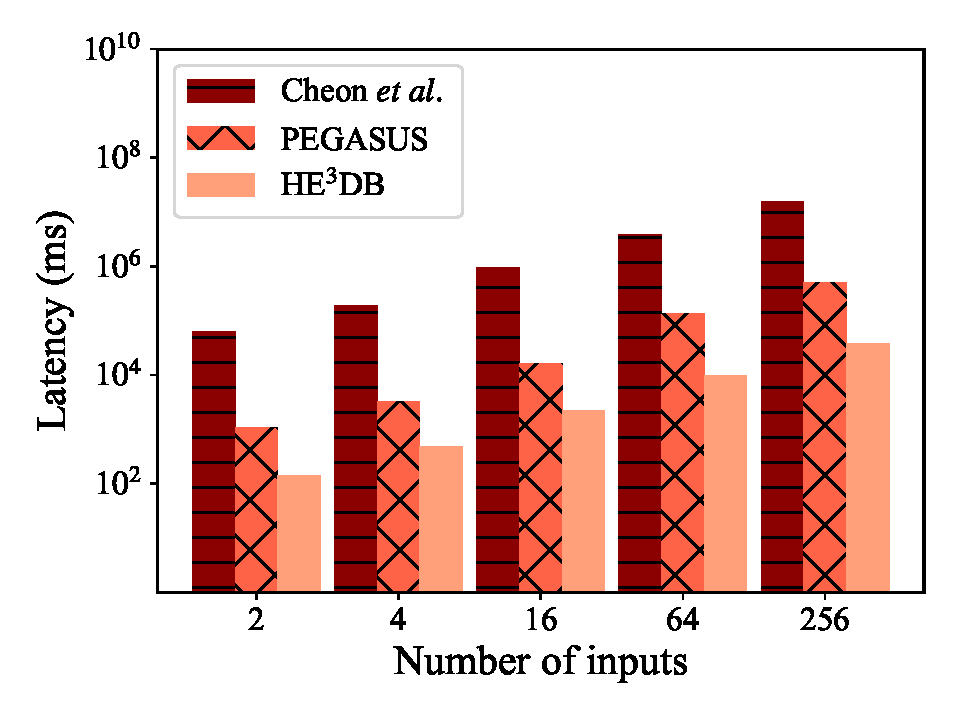
\includegraphics[width=\linewidth]{figure/minbench_4.pdf}
   %  % \vspace{-2em}
   %  \caption{4-bit}
   %  \label{fig:homminbench4}
   %  \end{subfigure}%
   %  \hfill
   %  \begin{subfigure}[b]{0.25\textwidth}
   %  \centering
   %  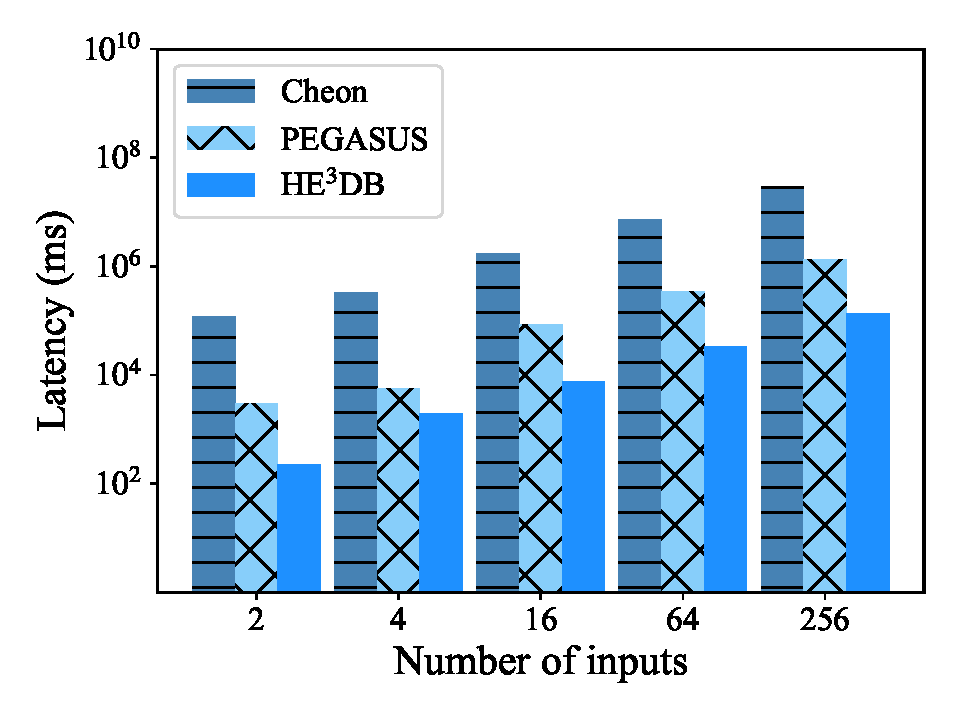
\includegraphics[width=\linewidth]{figure/minbench_8.pdf}
   %  % \vspace{-2em}
   %  \caption{8-bit}
   %  \label{fig:homminbench8}
   %  \end{subfigure}%
   %  \hfill
   %  \begin{subfigure}[b]{0.25\textwidth}
   %  \centering
   %  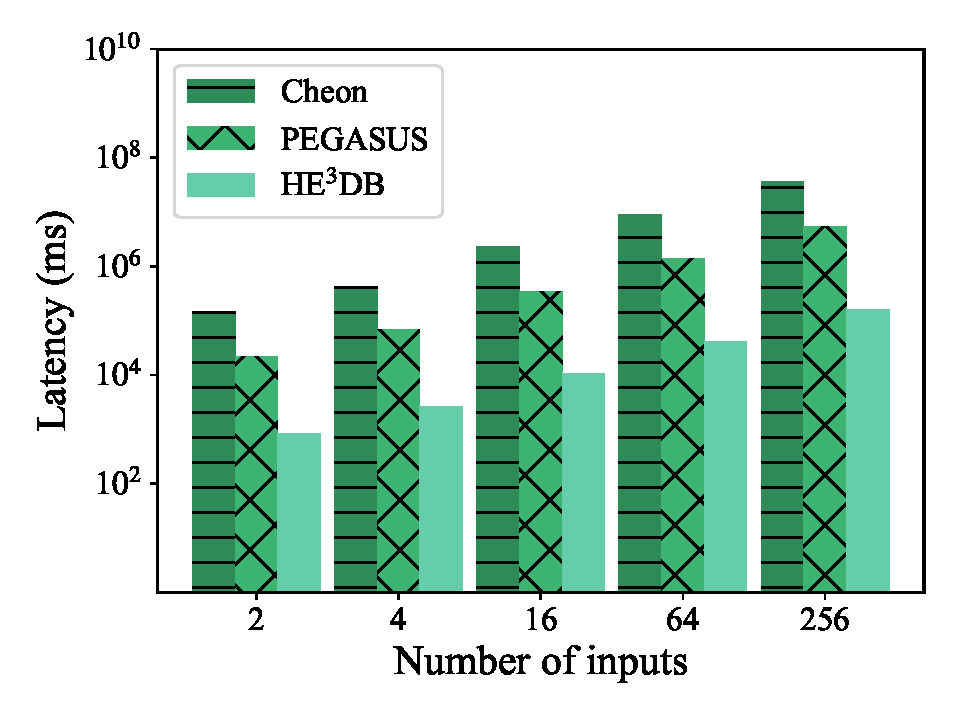
\includegraphics[width=\linewidth]{figure/minbench_12.pdf}
   %  % \vspace{-2em}
   %  \caption{12-bit}
   %  \label{fig:homminbench12}
   %  \end{subfigure}%
   %  \hfill
   %  \begin{subfigure}[b]{0.25\textwidth}
   %  \centering
   %  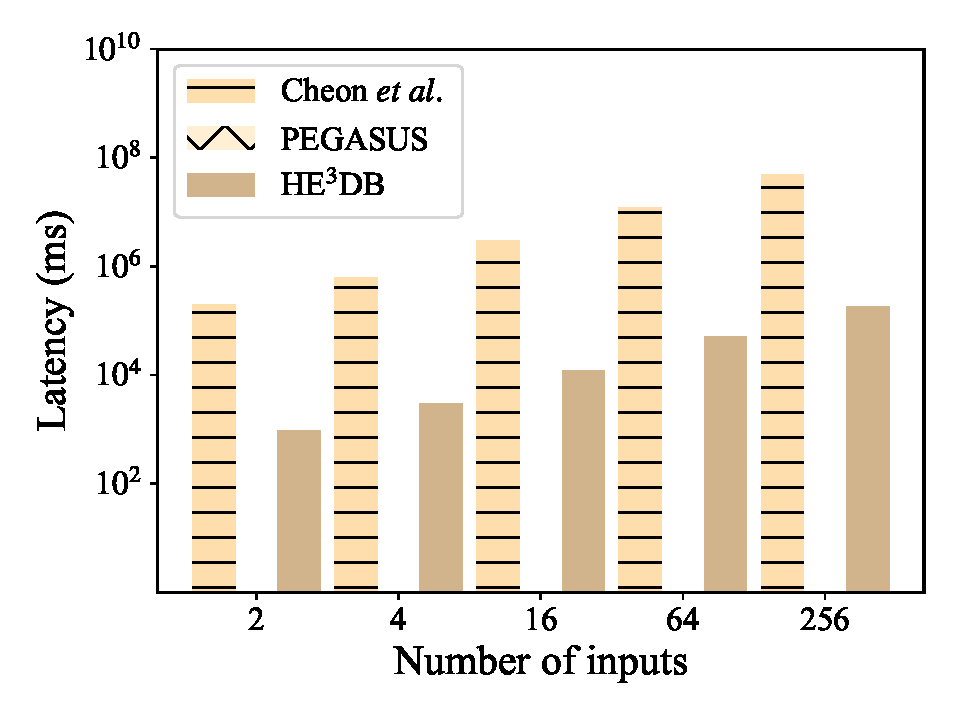
\includegraphics[width=\linewidth]{figure/minbench_16.pdf}
   %  % \vspace{-2em}
   %  \caption{16-bit}
   %  \label{fig:homminbench16}
   %  \end{subfigure}%
   
   % \end{center}
   %  % \vspace{-0.5em}
   %    \caption{Homomorphic MIN benchmark between $2,4,16,64,256$ numbers
   %          with $4,8,12$, and $16$ bits of precision.} 
   % \label{fig: homminbench}
   % \vspace{-0.5em}
\end{figure*}


%Here, we answer {\bf{RQ1}}. 
To answer {\bf{RQ1}}, we benchmark the efficiency of each of the 
cryptographic building blocks proposed in \cref{block},
including homomorphic comparison in \cref{block: comparison}, 
homomorphic \texttt{MIX/MAX} evaluation in \cref{block: minmax}
and ciphertext conversion in \cref{block: LWEsPack}. 
% The results
% are summarized as follows.

% {\bf{Homomorphic comparison}}:
%\subsubsection{Homomorphic comparison}
First of all, we compare the proposed $\homcomp$ with the best known 
existing works that support unbounded-depth predicate
evaluation, and the results are summarized in \cref{tab:combenchmark}.
We re-implement some of the existing works based on their open-source 
implementations~\cite{codepegasus, codesortinghat, codeopenfhe}
to fit our purpose (i.e., ciphertext-ciphertext comparison).
As observed in \cref{tab:combenchmark}, we are 7$\times$--113$\times$
faster than existing methods. Meanwhile, we can reduce the ciphertext
size by as much as 4.75$\times$ owing to our elastic ciphertext 
management policy.
% In addition,
% In \cref{tab:combenchmark}, we sketch the change
% of latency and ciphertext size on the predicate comparison operator $\geq$ 
% indifferent bits of precision.
% Specifically, in terms of latency, we achieve
% $24.67\times$, $19.07\times$, $8.13\times$ and $7.67\times$
% faster than the second best results on $4,8,12$, and $16$ bits of 
% precision, respectively.
In addition, as we can see from \cref{fig: homcompbench}, our
speedups are consistent across different comparison operators.
% shows the change of latency with 
% the increasing bits of precision for different methods. 
% As can be seen, our \NAME achieves lower latency
% compared to other methods on comparison operators $\geq, ==, >$, 
% which indicates higher efficiency.



%\subsubsection{Homomorphic \texttt{MIN/MAX}}
% {\bf{Homomorphic \dbmin/\dbmax}}: 
%\subsubsection{Homomorphic $\dbmin$/$\dbmax$ and $\orderby$}
Next, we compare the latency performance of the proposed homomorphic
\texttt{MIN/MAX} algorithms and SQL $\orderby$ operator to 
PEGASUS~\cite{pegasus} and Cheon \etal~\cite{ckkscomparison}
% and \NAME on the
% same numbers with the same bits of precision.
with a varying number of inputs and bit precision for the inputs.
As depicted in \cref{fig: homminbench} and \cref{fig: homsortbench},
our performance is on average around 
one order of magnitude faster than PEGASUS~\cite{pegasus},
and two orders of magnitude faster
than~\cite{ckkscomparison}.
Note in \cref{fig: homminbench} (b) and \cref{fig: homsortbench} (b) the 
histograms of PEGASUS~\cite{pegasus}
are left blank, for PEGASUS cannot support homomorphic \texttt{MIN/MAX} 
and $\orderby$ functions
over 16-bit operands.

%\subsubsection{Homomorphic ciphertext conversion}
% {\bf{Homomorphic Conversion}}: 
%\subsubsection{Homomorphic conversion}
% In ~\cref{tab:conversionbenchmark}, 
Lastly, to test the performance of the proposed $\repack$ operator, we
compare our algorithm to PEGASUS~\cite{pegasus} and 
Chen \etal~\cite{conversionhaochen}
over the task of converting $2^{15}$ LWE ciphertexts into
one RLWE ciphertext. Although PEGASUS~\cite{pegasus} achieves 
the lowest latency ($56s$), 
the method can only obtain $4$ bits of precision, which is 
not practical in most DB applications.
Although both the proposed $\repack$ and Chen \etal~\cite{conversionhaochen}
achieves higher precision ($\geq 16$ bits), \NAME
can be as much as $2 \times$ faster than~\cite{conversionhaochen}.

% \begin{table}[t!] 
%     \centering
%     \caption{Ciphertext converison benchmark}
%     \vspace{0em}
%         \begin{tabular}{ccc}
%             \toprule
%             Methods &  Precision (bit) & Latency (s)\\
%             \midrule
%             Pegasus~\cite{pegasus} &  4 & 56\\
%             Chen~\cite{conversionhaochen} & 20 & 230 \\
%             HE$^3$DB & 16 & 114 \\

%             \bottomrule
%         \end{tabular}
%     \label{tab:conversionbenchmark}
% \end{table}


\subsection{SQL Benchmarks}\label{eva: sql_benchmark}
To answer the \textbf{RQ2}, we test the end-to-end performance
of \NAME using the TPC-H benchmarks~\cite{tpc_h} and compare our results
with the corresponding works~\cite{sagma,heda}. Since
SAGMA~\cite{sagma} only uses HE for aggregation, the comparisons are
placed in the Appendix.
% We compare with SAGMA~\cite{sagma}, HEDA~\cite{heda}, and the method of 
% Kortekaa~\cite{aphadb} on the same task
% and evaluate the SQL queries in TPC-H benchmark.
% Moreover, we benchmark a data analysis model (decision tree) based on \NAME.


\begin{figure}[t!]
   \begin{center}
    \begin{subfigure}[b]{0.25\textwidth}
    \centering
    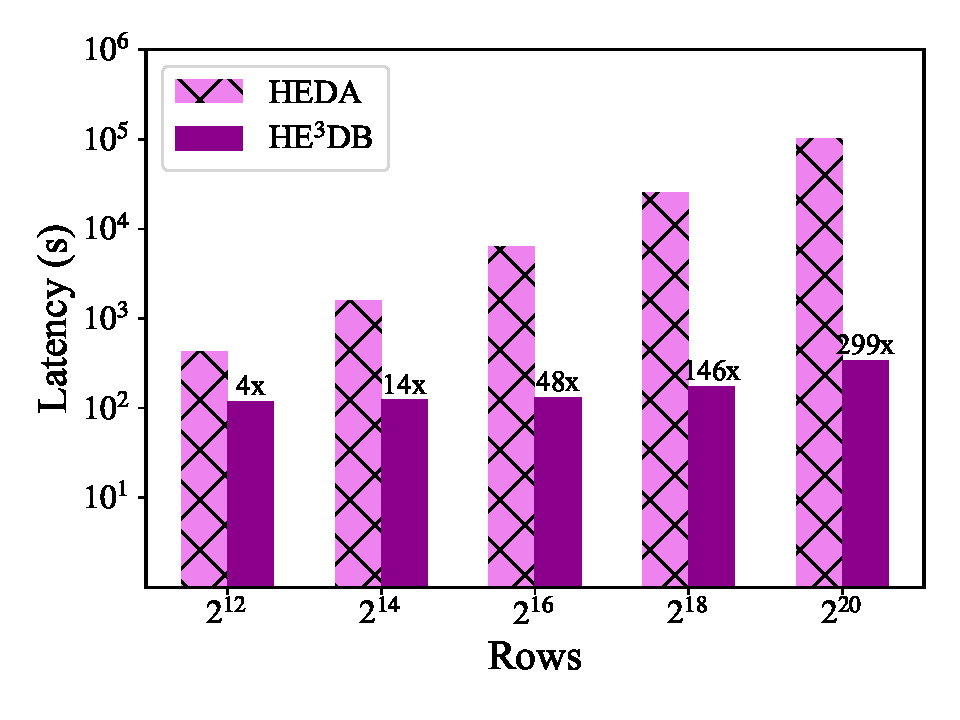
\includegraphics[width=\linewidth]{figure/compare_q1_heda.pdf}
    % \vspace{-1em}
    \caption{Query 1}
    \label{fig: hedaq1}
    \end{subfigure}%
    % \hfill
    \begin{subfigure}[b]{0.25\textwidth}
    \centering
    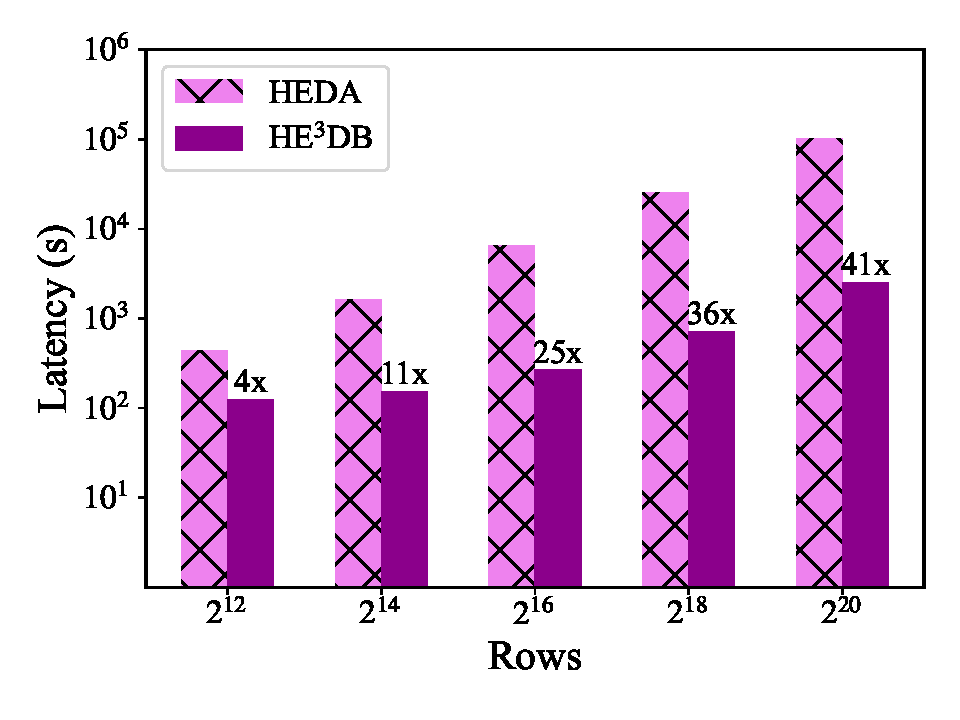
\includegraphics[width=\linewidth]{figure/compare_q6_heda.pdf}
    % \vspace{-1em}
    \caption{Query 6}
    \label{fig: heda16}
    \end{subfigure}%
    % \hfill
   \end{center}
    % \vspace{-1em}
      \caption{Comparison between \NAME and HEDA~\cite{sagma} on their modified TPC-H Query 1 and Query 6 with varying sizes of $\dbtabrow$.} 
      \Description{Comparison between \NAME and HEDA~\cite{sagma} on their modified TPC-H Query 1 and Query 6 with varying sizes of $\dbtabrow$.
      As the size of $\dbtabrows$ increases, 
      the advantage of our performance is more obvious.}
   \label{fig: hedabench}
   % \vspace{-0.5em}
\end{figure}

% {\bf{Aggregation Only}}:
%\paragraph{Aggreagation Only}


\begin{figure}[t!]
   \begin{center}
    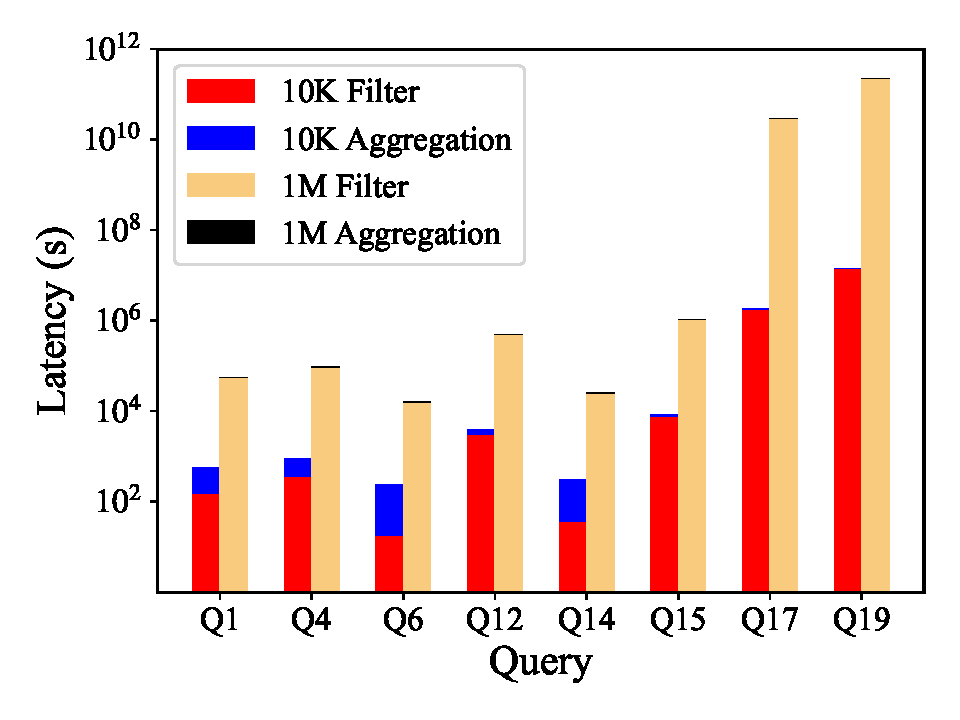
\includegraphics[width=0.9\linewidth]{figure/tpc_h.pdf}
   \end{center}
    % \vspace{-0.5em}
      \caption{Latency performance of \NAME on various TPC-H benchmark
      over different sizes of $\dbtabrow$.} 
      \Description{Latency performance of \NAME on various TPC-H benchmark
      over different sizes of $\dbtabrow$.
      As the size of the database increases, the bottleneck of the entire SQL lies in the filtering period.}
   \label{fig: tpchbench}
   % \vspace{-0.5em}
\end{figure}

% {\bf{TPC-H Benchmarks}}:
%\paragraph{TPC-H Benchmark}
We compare \NAME with HEDA, one of the most recent FHE-based encrypted DBMS
that supports unbounded-depth filter-aggregation~\cite{heda}. As shown in 
\cref{fig: hedabench}, on the same set of TPC-H queries, \NAME 
is on average $299\times$ faster on TPC-H Query 1 and $41\times$ faster on 
TPC-H Query 6. To closely examine the performance breakdown of \NAME,
we test a variety of the TPC-H benchmark queries on our \NAME framework, 
and the results are outlined in \cref{fig: tpchbench}. As the figure shows, while 
the filtering and aggregation latency are somewhat balanced on smaller databases,  
the filtering latency becomes the main performance bottleneck
as the size of the database gets larger. Overall, we can evaluate an end-to-end
SQL query over a 10K-row database within 241 seconds.

%\subsection{An End-to-End Decision Tree Benchmark}\label{eva:pdte}

% After query process, we use the function described in \cref{Analysis: Bridge} to bridge the gap between 
% aggregation result and data analysis. 
% {\bf{End-to-End Decision Tree Benchmark}}: 
%\paragraph{End-to-End Decision Tree Benchmark}
For the evaluation of the private decision tree, 
we provide a brief summary of the evaluation results obtained over
multiple decision tree models under a computation outsourcing setting, where both
the inputs and the model weights of the decision trees are ciphertexts.
% through our \pdte on 
% the experiment environment described \cref{eva:Arch}. 
To enable fair comparisons, we use the same datasets 
as in~\cite{sortinghat}, and reworked the implementation of~\cite{sortinghat} such that the
solution in~\cite{sortinghat} can also operate over encrypted inputs and model weights.
%\cref{fig: homtreebench} compares the performance of \NAME and \cite{sortinghat} on  
%end-to-end decision tree benchmark. 
While detailed comparison results can be found in the appendix, we achieve 12x--326x faster 
evaluation speed than~\cite{sortinghat} over a wide range of datasets and input sizes.
Thus, by adding the powerful online data analysis
capability to the expressive query evaluation framework,
\NAME is able to significantly improve the efficiency, usability
and practical applicability of outsourcing databases securely.
% able to significantly narrow
% the performance and usability gaps between theoretical FHE-based encrypted
% database constructions and practical needs for SDO in the real world.
% improve the 
% practicality of secure database outsourcing based on fully homomorphic encryption.


\section{Conclusions}
In this work, we propose \NAME, an FHE-based encrypted database framework
that enables expressive SQL statements to be efficiently 
queried on large-scale encrypted DBMS. 
We observe that a new FHE infrastructure needs to be developed 
to meet the usability, security, and efficiency demands from
the encrypted DBMS. By designing comparison, aggregation, and
conversion operators specifically for encrypted databases, we can
outperform the best-known FHE algorithms on all DB-related task benchmarks.
In particular, we are able to achieve
$41\times$--$299\times$ reduction in query latency against the 
state-of-the-art FHE-based encrypted database solution
on a 1M-record encrypted database.
% We observe that, 
% while application-specific FHE algorithms are fast, such algorithms
% do not handle complex DB queries well due to 
% usability constraints. In contrast, general FHE algorithms are highly
% usable but tend to be slow. 

% In conclusion, it is rarely a good idea to include the same section three times in 
% a paper, or to have a conclusion that does not conclude.


% \input{ccs-body/cfp.tex}
% \input{ccs-body/cfp.tex}
% \input{ccs-body/cfp.tex}



% \input{ccs-body/cfp.tex}

\begin{acks}
% TODO: For the submission, don't include acknowledgments since they would most likely deanonymize you.
\end{acks}
 % TODO: replace with your brilliant paper!
\clearpage
\bibliographystyle{ACM-Reference-Format}
\bibliography{main}
% \clearpage
\appendix
\renewcommand{\tablename}{Appendix Table}
\setcounter{table}{0}
\renewcommand{\thetable}{A\arabic{table}}
\renewcommand{\tablename}{Appendix Table}
\setcounter{algorithm}{0}
\renewcommand{\thealgorithm}{A\arabic{algorithm}}
\renewcommand{\figurename}{Appendix Figure}
\setcounter{figure}{0}
\renewcommand{\thefigure}{A\arabic{figure}}
\setcounter{equation}{0}
\renewcommand{\theequation}{A\arabic{equation}}
\section{Full Notations and operators}
We summarize the notations and operators used
in this work in \cref{tab: notations}.

\begin{table}[t!] 
% \addtolength{\tabcolsep}{-2pt}
% \footnotesize
   \begin{center}
   \vspace{-0em}
       \caption{Summary of Notations}\label{tab: notations}
       \vspace{-0em}
     \begin{tabular}{c|l}
        \toprule[1.0pt]
        Notation & Description \\
        \midrule
        $\db$ &  The database \\
        $\dbtab$ &  The data tables in the database \\
        $\dbtabrowsize$ & The number of rows in table $\dbtab$ \\
        $\dbtabcolsize$ & The number of columns in table $\dbtab$ \\
        $\dbquery$  & The SQL query.\\
        $\dbabsquery$  & The number of predicates in query $\dbquery$.\\
        $\mathcal{M}$ &  The data analysis model\\
        $\algoweight$ & The parameters in data analysis model \\
        \midrule
        $\lambda$ & The security parameter\\
        $p$       & The plaintext modulus \\
        $q$       & The ciphertext modulus for $\lwe$\\
        $Q$       & The ciphertext modulus for $\rlwe$\\
        $Q'$       & The ciphertext modulus for $\rgsw$\\
        $n$       & The lattice dimension for $\lwe$\\
        $N$       & The lattice dimension for an $\rlwe$\\
        $N'$       & The lattice dimension for an $\rgsw$\\
        $l$       & The number of $\rlwe$ in $\rgsw$ \\
        % $\mathbb{Z}_q$ & The ring of integers modulo $q$ \\
        $\mathbb{Z}_{q}^{n}$ & The set of n-vectors over $\mathbb{Z}_q$ \\
        % $\mathbb{Z}[X]$ & The polynomial ring over $\mathbb{Z}$ \\
        % $\mathbb{Z}_{q}[X]$ & The polynomial ring over $\mathbb{Z}_q$ \\
        $R$ & The cyclotomic ring   $\mathbb{Z}[X]/(X^N+1)$\\
        $R_{Q} $ & The cyclotomic ring $\mathbb{Z_{Q}}[X]/(X^N+1)$ \\
        $\chi$ & The noise distribution \\
        $\Delta$ & The scaling factor \\
        $\mathbf{a}$ & An element in vector domain \\
        $\mathbf{a}_i$ & The i-th element of $\mathbf{a}$ \\
        $ \Tilde{a} $ & An element in polynomial ring \\
        $ \Tilde{a}_i $ & The i-th coefficient of $\Tilde{a}$ \\
        $ \mathbf{A} $ & An element in matrix domain \\
        $\mathfrak{d} $ & The number of the leaf nodes\\
        % $ \hat{a} $ & The NTT-domain of element $a$ \\
        \midrule
        \multirow{2}{*}{$ \lwe^{n, q}_{\bs}(m) $} & An LWE ciphertexts encrypting $m$ \\
        & with parameters $(n, q)$ and secret $\bs$\\
        \multirow{2}{*}{$ \rlwe^{N, Q}_{\tts}(\ttm) $} & An RLWE ciphertexts encrypting $\ttm$ \\
        & with parameters $(N, Q)$ and secret $\tts$\\
        \multirow{2}{*}{$ \rgsw^{N', Q'}_{\Tilde{\bs}}({\bf{m}})$} & An RGSW ciphertext encrypting
        {\bf{m}} \\
        & with parameters $(N', Q')$ adn secret $\Tilde{\bs}$ \\
        $\diamond $ & Homomorphic matrix-vector multiplication\\
        %$ +, -, \cdot$ & Addition, subtraction and multiplication \\
        $ \cmux $  & Homomorphic selector~\cite{DBLP:journals/joc/ChillottiGGI20}\\
        $ \pbs  $ &  Programmable bootstrapping~\cite{DBLP:conf/asiacrypt/tfhepbs} \\
        $ \homgate$  & Homomorphic gate~\cite{DBLP:conf/eurocrypt/DucasM15, DBLP:journals/joc/ChillottiGGI20}\\
        $\bar{ct}$ & The NOT gate result of $ct$ \\
        \multirow{2}{*}{$\sei$} & Converting RLWE to LWEs \\
                & (a.k.a, sample extract index~\cite{DBLP:journals/joc/ChillottiGGI20}) \\
        \multirow{2}{*}{$\repack$} & Converting LWEs to RLWE \\
        & (a.k.a, repack~\cite{pegasus,conversionhaochen}) \\
        \multirow{2}{*}{$\cb$} & Converting LWE to RGSW \\
        & (a.k.a., circuit bootstrapping~\cite{DBLP:journals/joc/ChillottiGGI20}) \\
        \bottomrule[1.0pt]
     \end{tabular}
   \end{center}
    \vspace{-0em}
\end{table}
\begin{figure*}[t!]
   \begin{center}
    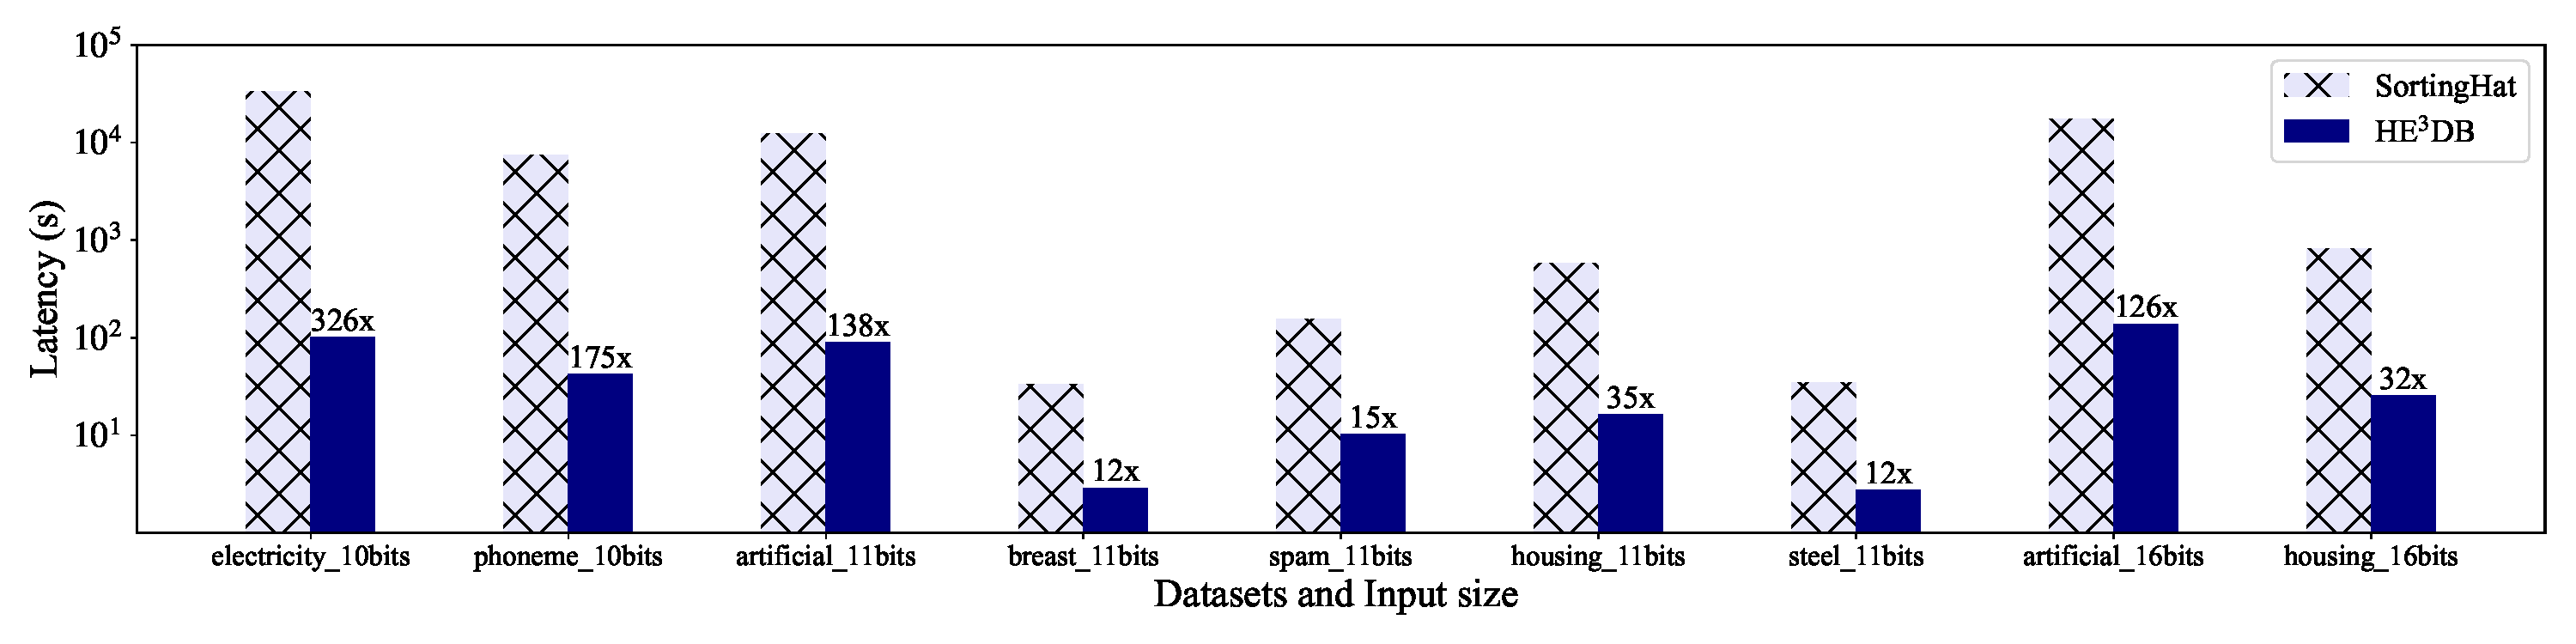
\includegraphics[width=\linewidth]{figure/treebench.pdf}
   \end{center}
    \vspace{-0.5em}
      \caption{Running time of our PTDE algorithm compared to SortingHat~\cite{sortinghat}} 
   \label{fig: homtreebench}
   \vspace{-0.5em}
\end{figure*}

\begin{algorithm}[t!]
    % \tiny
    \caption{\br}
    \label{algo: kHMSB}
    \SetKwInOut{Input}{Input}\SetKwInOut{Output}{Output}\SetKwInOut{Return}{Return}
    \Input{A Test polynomial $\Tilde{v} = v_0 + v_1x + ... + v_{N-1}x^{N-1}$.}
    \Input{An LWE ciphertext $ct = \lwe_{\mathbf{s}}^{n,q}(m) = (b, \mathbf{a})$.}
    \Input{A bootstrapping key $\bBK$, where 
    $\bBK\left[i\right] = \rgsw^{N',Q'}_{\Tilde{s}}(\mathbf{s}_{i})$, for $i \in [1,n]$}
    \Output{A LWE ciphertext $ct_{O} = \lwe_{\mathbf{s}}^{n,q}(v_{m})$.}
    $b \leftarrow \round{\frac{2N}{q}b} $ 
    and $\mathbf{a} \leftarrow \round{\frac{2N}{q}\mathbf{a}_{i}}$. \\
    $\Tilde{v} \leftarrow \mu \cdot (1 + x^2 + x^3 + ... + x^{N-1}) $ \\
    Initialize $ACC \leftarrow X^{-b}\cdot (\Tilde{v}, 0) \in \rlwe_{\Tilde{s}}^{N,Q}(.)$. \\
    \For { $i = 0$ \KwTo $n-1$}
    {
        $ACC \leftarrow \cmux(\bBK_{i}, X^{-\mathbf{a}[i]} \cdot ACC, ACC)$
    }
    $ct_{O} \leftarrow \sei(ACC)[0]$ \\
    \Return{$ct_{O}  
    = \lwe_{\mathbf{s}}^{n,q}(v_{m})$}
\end{algorithm}

\begin{algorithm}[t!]
    % \tiny
    \caption{$\kappa$-bit $\pbshmsb$}
    \label{algo: kHMSB}
    \SetKwInOut{Input}{Input}\SetKwInOut{Output}{Output}\SetKwInOut{Return}{Return}
    \Input{A LWE ciphertext $ct_{I} = \lwe^{n,q}_{\mathbf{s}}(m) 
    = (b, \mathbf{a})$, where $m \ in [0, 2^{k} -1]$.}
    \Input{A constant $\mu = q / 4$.}
    \Input{A bootstrapping key $\bBK$, where 
    $\bBK\left[i\right] = \rgsw^{N',Q'}_{\Tilde{s}}(\mathbf{s}_{i})$, for $i \in [1,n]$}
    \Output{A LWE ciphertext $ct_{O} = \lwe_{\mathbf{s}}^{n,q}(\msb(m))$.}
    % $b \leftarrow \lfloor \frac{2N}{q}b \rceil$ 
    % and $\mathbf{a} \leftarrow \lfloor \frac{2N}{q}\mathbf{a} \rceil$ \\
    $\Tilde{v} \leftarrow \mu \cdot (1 + x^2 + x^3 + ... + x^{N-1}) $ \\
    $ACC \leftarrow \br(\Tilde{v}, ct_I, \mathbf{BK})$ \\
    $ct_{O} = (b', \mathbf{a'}) \leftarrow \sei(ACC)[0]$ \\
    \Return{$ct_{O} = (b' + \mu, \mathbf{a}) 
    = \lwe_{\mathbf{s}}^{n,q}(\msb(m))$}
\end{algorithm}

% \begin{algorithm}[t!]
%     % \footnotesize
%     \caption{\texttt{1-out-of-k-CMUX}}
%     \label{algo: kcmux}
%     \SetKwInOut{Input}{Input}\SetKwInOut{Output}{Output}\SetKwInOut{Return}{Return}
%     \Input{$k$ $(\ge 2)$ LWE ciphertexts
%     $ct_0, ct_1, ...,ct_{k-1}$.}
%     \Input{$k-1$ control signals $C_1, C_2, ..., C_{k-1}$ where $C_t = 
%     \rgsw(1)$ and else are $\rgsw(0)$}
%     \Output{An LWE ciphertext $ct_{O} = ct_t$}
%     Initialize $ACC \leftarrow ct_0$. \\
%     \For{$i = 1$ \KwTo $k - 1$}
%     {
%         $temp_i \leftarrow ct_i - ct_0$ \\
%         $ACC \leftarrow ACC + temp_i \odot C_i$
%     }
%     \Return{$ACC$}
% \end{algorithm}

% \begin{algorithm}[t!]
%     % \tiny
%     \caption{Optimized Homomorphic \texttt{MIN} Aggreagation \texttt{OpHomMINAgg}}
%     \label{algo: ophomminagg}
%     \SetKwInOut{Input}{Input}\SetKwInOut{Output}{Output}\SetKwInOut{Return}{Return}
%     \Input{An RLWE ciphertext of the aggregated column $ct = \rlwe(\Tilde{m}), 
%     \Tilde{m}_i = m_i, i \in \mathbb{Z}_{\dbtabrowsize}$.}
%     \Input{Filtered result $cf=
%     (cf_{1}, cf_{2}, ... ,cf_{\dbtabrowsize})$, where
%     $cf_i = \lwe(f_i)$, $f_i = 0$ or $1$.}
%     \Input{The Pre-defined constant $\lwenan$.}
%     \Input{A bootstrapping key $\bBK$.}
%     \Output{A LWE ciphertext $ct_{O} = \lwe(\dbmin(m_{t_1}, ...,m_{t_f}))$ where
%     $f =  {\textstyle \sum_{i=0}^{\abs{\mathcal{T}}_{r}}}f_i$
%     and $f_{t_1}, f_{t_2}, ..., f_{t_{f}} = 1$.}
%     $\mathbf{ct} = \sei(ct) = (ct_1, ct_2, ...,ct_{\dbtabrowsize})$ \\
%     \For{$i = 1$ \KwTo $\frac{\dbtabrowsize}{2}$}
%     {
%         $c = \homcomp(ct_{2i-1}, ct_{2i}, \leq)$ \\
%         $c_1 = \homgate(cf_{2i-1}, \bar{cf_{2i}}, \reg{AND}) + 
%                \homgate(
%                \homgate(cf_{2i-1}, cf_{2i}, \reg{AND}), c, \reg{AND})$ \\
%         $c_2 = \homgate(cf_{2i}, \bar{cf_{2i-1}}, \reg{AND}) + 
%                \homgate(
%                \homgate(cf_{2i-1}, cf_{2i}, \reg{AND}), \bar{c}, \reg{AND})$ \\
%         $C_1 = \cb(c_1, \bBK)$ \\
%         $C_2 = \cb(c_2, \bBK)$ \\
%         $ct_{2i} = \texttt{1-out-of-3-CMUX}
%         (C_1, C_2, ct_{2i-1}, ct{2i}, \lwenan)$ \\
%     }
%     \For{$i = 2$ \KwTo $\log_{2}{\dbtabrowsize}$}
%     {
%         \For{$j = 1$ \KwTo $2^{\log_{2}{\dbtabrowsize} - i}$}
%         {
%             $ct_{2^{i}j} = \hommin
%             (ct_{2^{i}j-2^{i-1}}, ct_{2^{i}j}, \bBK)$ \\
%         }
%     }
%     \Return{$ct_{O} = ct_{2^{n}}$}
% \end{algorithm}

% \begin{lemma}
%     The output of \cref{algo: ophomminagg} is equal to 
%     \cref{algo: homminagg} and 
%     the number of homomorphic \texttt{CMUX} gates is 
%     $\frac{\abs{\mathcal{T}}_{r}}{2} -1$, 
%     the number of homomorphic \texttt{1-out-of-3 CMUX} gates is 
%     $\frac{\abs{\mathcal{T}}_{r}}{2}$.
%     the number of homomorphic 
%     \texttt{LWEToRGSW} instructions is 
%     $\frac{3\abs{\mathcal{T}}_{r}}{2} -1)$,
%     the number of homomorphic 
%     \texttt{HomCom} instructions is
%     $\abs{\mathcal{T}}_{r}-1$.
%     \label{lemma: ophomminagg}
% \end{lemma}

\section{Proof for Lemma 4.1 and Lemma 4.2}
\begin{proof} \textbf{\cref{lemma: homcomp}}
    First, we prove the correctness of the \cref{algo: homcom}.
    If the comparison operator is $\geq$, 
    the line 2 in \cref{algo: homcom} results 
    $\lwe(\texttt{NOT}(\msb(a-b))$.
    the predicate $a \geq b$ is equal to $\msb(a - b) == 0$.
    If $a \geq b$, the predicate is True, and $\lwe(\texttt{NOT}(\msb(a-b)) = \lwe(1)$. 
    If $a < b$, the predicate is False, and $\lwe(\texttt{NOT}(\msb(a-b)) = \lwe(0)$. 
    Other comparison operators are the same.
    The number of $\pbs$ in \cref{algo: homcom}
    includes the $\pbs$ in $\hmsb$ and $\homgate$.
    From \cref{algo: tkHMSB}, the number of $\pbs$ 
    evaluated in a $tk$-bit ciphertext
    MSB extraction is $2 \times (t - 1) + 1 = 2t - 1$.
    Meanwhile, one $\homgate$ 
    includes one $\pbs$ as we discussed in \cref{pre:he_circuits}.
    Thus, the number of $\pbs$ in \cref{algo: homcom} 
    is $2t-1$ when the comparison operator is $>,<$ and  $2t$  when the comparison operator is $\geq, \leq, ==, \ne$.
\end{proof}

\begin{proof} \textbf{\cref{lemma: homminagg}}
    In \cref{algo: homminagg}, the first for loop (line 2-4)
    includes $\dbtabrowsize$ $\cb$ and $\cmux$, the second for loop (line 5-7)
    contains $2^{\log_{2}{\dbtabrowsize - 1}} + 2^{\log_{2}{\dbtabrowsize - 2 }} 
    + ... + 2^{0} = \dbtabrowsize - 1$ $\hommin$.
    As shown in \cref{algo: hommin}, each $\hommin$ has one $\homcomp$, 
    one $\cb$ and one $\cmux$.
    Therefore, the total number of $\cmux$ gates is $\dbtabrowsize + \dbtabrowsize - 1 = 2\dbtabrowsize - 1$, the whole number of $\cb$ operators is 
    $\dbtabrowsize + \dbtabrowsize - 1 = 2\dbtabrowsize - 1$, the number of 
    $\homcomp$ is $\dbtabrowsize - 1$.
    \label{proof: homminagg}
\end{proof}


 % \begin{proof} \textbf{\cref{lemma: ophomminagg}}
 %     We
 %     \label{proof: ophomminagg}
 % \end{proof}


\section{Additional Comparisons against SAGMA}
\begin{figure}[t!]
   \begin{center}
    \begin{subfigure}[b]{0.25\textwidth}
    \centering
    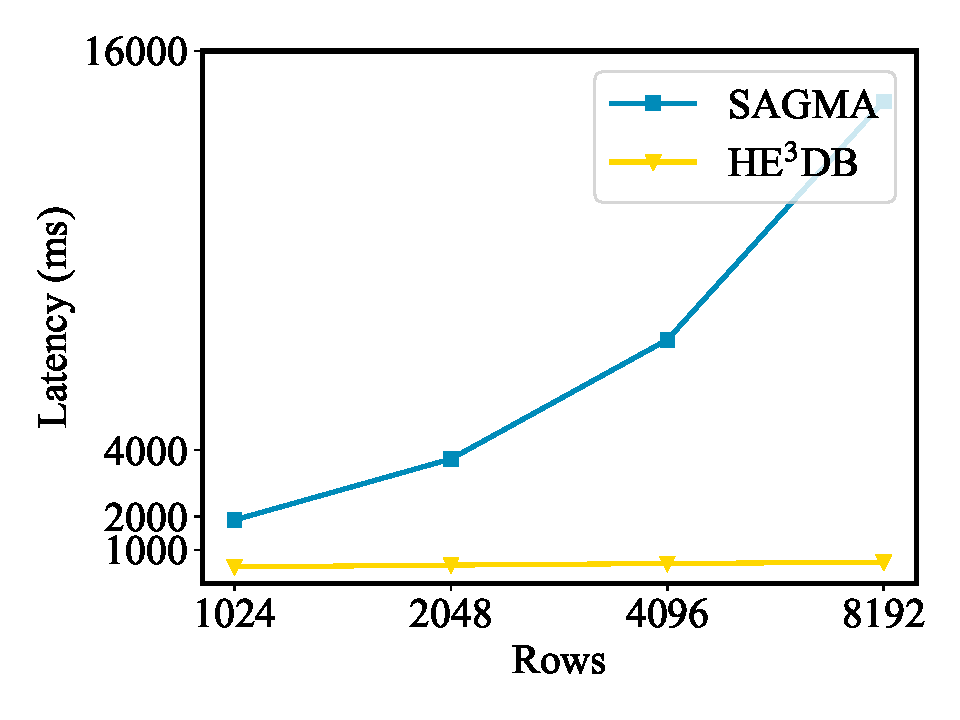
\includegraphics[width=\linewidth]{figure/benchmark_count.pdf}
    % \vspace{-1em}
    \caption{$\dbcount$}
    \label{fig: aggcount}
    \end{subfigure}%
    % \hfill
    \begin{subfigure}[b]{0.25\textwidth}
    \centering
    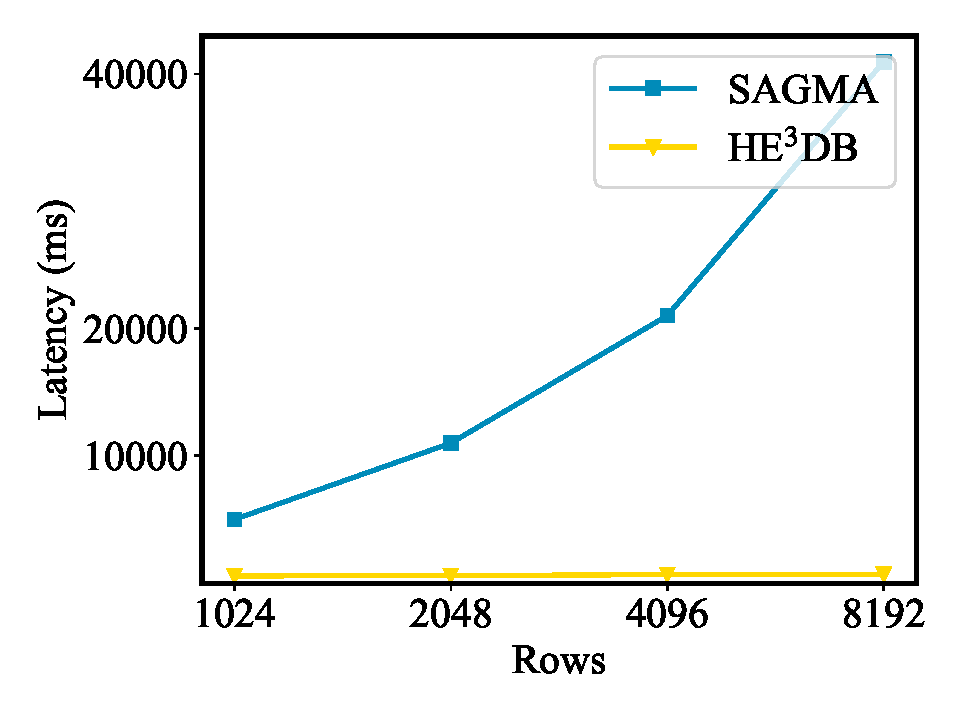
\includegraphics[width=\linewidth]{figure/benchmark_sum.pdf}
    % \vspace{-1em}
    \caption{$\dbsum$}
    \label{fig: aggsum}
    \end{subfigure}%
    % \hfill
   \end{center}
    % \vspace{-1em}
      \caption{Comparison with SAGMA~\cite{sagma} on aggregation function $\dbcount$ and $\dbsum$.} 
      \Description{Comparison with SAGMA~\cite{sagma} on aggregation function $\dbcount$ and $\dbsum$.}
   \label{fig: aggbench}
   % \vspace{-0.5em}
\end{figure}
As SAGMA~\cite{sagma} only uses HE 
in its aggregation process,
we only compare \NAME with SAGMA on the arithmetic aggregation tasks.
As shown in \cref{fig: aggbench}, we can obtain $23\times$ and 
$58\times$ faster in $\dbcount$ and $\dbsum$ operations on a 8192-row database, respectively.

\section{Evaluating Private Outsourced Decision Tree}
\begin{algorithm}[t!]
\caption{\texttt{PDTEval} based on $\homcomp$}
\label{algo:pdte}
 \SetKwInOut{Input}{Input}\SetKwInOut{Output}{Output}\SetKwInOut{Return}{Return}
\Input {Private decision tree Model $\mathcal{CM}$=\{$(ct_0, ..., ct_{2\mathfrak{d}-2}),\\ (a_0, ..., a_{2\mathfrak{d}-2}),(cw_0, ..., cw_{\mathfrak{d}-1})$\}}
\Input {Query results $\mathcal{CR}$= $(cr_0, cr_1, ..., cr_{\lvert G \rvert})$}
\Output{ $\mathfrak{d}$ values of leaves: ${z_0}, ..., {z_{\mathfrak{d}-1}}$}
\State Initialize root value $v_0$ as ${\rm LWE}^{n,q}_{\mathbf{s}}(1)$\\
\State Initialize other node value $v_j$ as ${\rm LWE}^{n,q}_{\mathbf{s}}(0), j \in \left\{ 1, ..., 2\mathfrak{d}-2 \right\}$\\
\For {$i = 0$ \KwTo  $2\mathfrak{d}-2$}{
    \State${cb_i}\leftarrow\; \texttt{HomComp}({cr_{a_i}},{ct_i},\ge )$
}
\For { $i = 1$ \KwTo $\log{\mathfrak{d}}$}{
\For {$j = 0$ \KwTo   $2^{i-1}-1$}{
\State$v_{2^i + 2*j }\leftarrow\; \texttt{HomGate}({cb_{2^{i-1}-1 + j}},v_{2^{i-1}-1 + j}, \texttt{AND})$
\State$v_{2^i + 2*j- 1}\leftarrow\; v_{2^{i-1}-1 + j} - v_{2^i + 2*j}$}
}
\For { $i = 0$ \KwTo $\mathfrak{d}-1$}{
\State${z_i}\leftarrow\; v_{2^{\log \mathfrak{d}}-1+i}$}
\Return{${z_0},...,{z_{\mathfrak{d}-1}}$}
\end{algorithm}
A private decision tree model $\mathcal{CM}$ includes the encryption of threshold $ct_i$, the attribute index $a_i$ and the encryption of label $cw_i$. \cref{algo:pdte} shows our PDTE algorithm, which involves the following steps:\\
\step{Line 1-2, Initialization}:
Server initializes the value of each node as the encryption of 0, denoted by $v_j$ for all $j \in \{0,...,\mathfrak{d}-2\}$, except the root, denoted by $v_0$,  which contains the encryption of 1.\\
\step{Line 3-5, Comparison}:
For each decision node $i$, server computes the Homomorphic Comparison function ${cb_i} \leftarrow [cr_{a_{v}} \ge ct_i}]$, we denote the controller bit of each node by ${cb_i}$ corresponding to the node $i$
for $i$ $\in \{0,...,\mathfrak{d}-2\}$.\\
\step{Line 6-10, Traversal}:
Then the server moves root value ${v_0}$ from the root to a desired leaf. The path depends on the controller bits on each node. Take node $i$ as an example, if node $i$ has value ${v_i}$ and the controller bit of $i$ is ${cb_i}$, the value of the left child node (denoted by ${v_{Lci}}$)and the right child node (denoted by ${v_{Rci}}$) are compute as ${v_{Rci}} = \texttt{HomAND}({cb_i}, {v_i})$, 
${v_{Lci}} = {v_i} - {v_{Rci}}$. After traversal, the value of the root (which is the encryption of 1) is copied to the desired place.\\
Finally, only one leaf has a value which is the encryption of 1, we can easily get this unique label value.\\

{\bf{Evaluation Results}}: As shown in \cref{fig: homtreebench}, 
since SortingHat~\cite{sortinghat} does not target
on evaluating private decision under a secure computation outsourcing setting, we can achieve
up to 300$\times$ speedup using \cref{algo:pdte}.


% The algorithm involves the following steps:
% First, server computes the homomorphic comparison function between threshold value and correspond input attribute for each decision node $i$, restore the comparison result as controller bits ${cb_i}$. Second, server traverses the tree, moves root value $v_0$ from the root to a desired leaf. The path depends on the controller bits on each node. Take node $i$ as an example, if node $i$'s controller bits ${cb_i}$ is the encryption of 1, then copy the node value to its right child  and the left child node value becomes the encryption of 0. Otherwise, vice versa. After traversal, the value of root (which is the encryption of 1) is copied to the desired place. Finally we use homomorphic multiplication to obtain the analysis result.
%For the detailed \texttt{PDTEval} description, see the appendix.

% In \cref{eva:pdte}, we demonstrate that our \pdte function achieves 12x to 326x better evaluation time on different datasets and input size compared with existing work \cite{sortinghat}.


\end{document}
